\documentclass[%
 reprint,
 nofootinbib,
 amsmath,amssymb,
 aps,
 floatfix,
]{revtex4-2}

% Packages and macros of the report (included by main.tex)

\usepackage[utf8]{inputenc}
\usepackage{graphicx}
\usepackage{dcolumn}
\usepackage{bm}
\usepackage{enumitem}
\usepackage{comment}
\usepackage{siunitx}
\usepackage{booktabs}
\usepackage{placeins}
\usepackage{hyperref}
\hypersetup{colorlinks = true, linkcolor = blue!55!black, citecolor = blue!55!black, urlcolor = blue!55!black}
\usepackage{amsfonts}
\usepackage{nicefrac}
\usepackage{microtype}
\usepackage{amsmath}
\usepackage{mathtools}
\usepackage{multirow}
\usepackage{xcolor}
\usepackage{xspace}

\renewcommand{\thefigure}{\Roman{figure}}

% unit / symbol macros, mirroring the style used in lhc_anomaly_detection/main.tex
\newcommand{\GeV}{\ensuremath{\,\text{Ge\hspace{-.08em}V}}\xspace}
\newcommand{\MeV}{\ensuremath{\,\text{Me\hspace{-.08em}V}}\xspace}
\newcommand{\Araw}{\ensuremath{A_{\mathrm{raw}}}\xspace}
\newcommand{\ACP}{\ensuremath{A_{CP}}\xspace}

% Left-aligned, justified cell of fixed width inside a tabular (replaces p{...} columns, which revtex4-2 breaks with array >= 2.7)
\newcommand{\pcell}[2]{\parbox[t]{#1}{\leftskip=0pt\rightskip=0pt\parfillskip=0pt plus 1fil\relax #2}}

% TODO markers -- remove once every section has real content
\newcommand{\todo}[1]{\textcolor{red}{\textbf{[TODO: #1]}}}

% allow two wide floats on the top of a page (results figures cited together)
\renewcommand{\dbltopfraction}{0.85}
\renewcommand{\dblfloatpagefraction}{0.7}
\setcounter{dbltopnumber}{3}

\usepackage{xspace}\newcommand{\appref}[1]{\unskip~(Sec.~\ref{#1})\xspace}\newcommand{\apprefs}[2]{\unskip~(Secs.~\ref{#1} and~\ref{#2})\xspace}

\begin{document}
\pagestyle{plain}

\title{Frequentist and Bayesian Analysis of the Matter--Antimatter Asymmetry in $B^{\pm} \to K^{\pm} K^{+} K^{-}$ Decays at LHCb\\[2.0ex]
\small Final project for the \textit{Statistics and Data Analysis} course\\
\small Academic Year 2025--2026}

\author{Marco Belotti}
\author{Giacomo Moretti}
\affiliation{Università degli Studi di Milano-Bicocca}


\begin{abstract}
We measure the raw charge asymmetry $\Araw=[N(B^-)-N(B^+)]/[N(B^-)+N(B^+)]$ of $B^{\pm}\to K^{\pm}K^{+}K^{-}$ decays in the 2011 LHCb Open Data record and compare two inference frameworks on the same data and the same question: an extended unbinned maximum-likelihood fit with profile likelihood and a Bayesian analysis sampled with Markov chain Monte Carlo (MCMC). After a common preselection ($19{,}731$ candidates in the fit window), a common mass model gives $\Araw=-0.0441\pm0.0085\,(\text{stat})\pm0.0072\,(\text{syst})$ in the Frequentist fit and $-0.0443\pm0.0085\pm0.0070$ in the Bayesian one, $5.2$ standard deviations from zero (Bayes factor $\approx9\times10^3$ against no asymmetry). The two methods agree in value, uncertainty and coverage, which was verified on toy-MC experiments; the dominant systematic uncertainty is the particle-identification requirement. The asymmetry is not uniform over the Dalitz plane: in the region of the published analysis of the same data we find $\Araw=-0.234\pm0.025$, reproducing $-0.239\pm0.020$. A machine-learning selection trained on weak labels, described in Sec.~\ref{sec:ml}, leaves $\Araw$ unchanged within its statistical spread. $\Araw$ is not corrected for production and detection asymmetries and is therefore not a measurement of $\ACP$.
\end{abstract}

\maketitle
\setcounter{tocdepth}{2}
\tableofcontents

\section{Introduction}
\label{sec:intro}
Charge-parity (CP) violation -- the small observed asymmetry between the behavior of matter and antimatter -- is one of the necessary ingredients for the matter-dominated universe we observe, yet the CP violation built into the Standard Model is far too small to account for it. Studying CP violation in the decays of $B$ mesons, where it is comparatively large and experimentally accessible, is one of the main ways to test the Standard Model's Cabibbo-Kobayashi-Maskawa (CKM) description of the effect and search for physics beyond it. Charmless three-body decays such as $B^{\pm}\to h^{\pm}h^{+}h^{-}$ ($h=K,\pi$) are especially interesting in this respect: unlike a two-body decay, the three-body phase space (the Dalitz plot) allows the asymmetry to be studied not only as a single global number, but also \emph{locally}, since interference between intermediate resonances can concentrate CP-violating effects in specific kinematic regions rather than spreading them uniformly~\cite{lhcb_cpv_prd2023,lhcb_cpv_paper}.
The quantity measured in this work is the raw asymmetry between the signal yields of the two charges,
\begin{equation}
\Araw=\frac{N(B^-)-N(B^+)}{N(B^-)+N(B^+)} .
\label{eq:araw}
\end{equation}
It differs from the physical asymmetry $\ACP$ by the production asymmetry $A_P$ of $B^\pm$ mesons in $pp$ collisions and by the detection asymmetry $A_D$ of the final state; to first order in these small quantities,
\begin{equation}
\ACP\approx\Araw-A_P-A_D ,
\label{eq:acp}
\end{equation}
where $A_D$ arises mainly from the different interaction cross sections of $K^+$ and $K^-$ with the detector material and depends on the kaon momenta~\cite{lhcb_cpv_prd2023}. Neither correction is applied here, so $\Araw$ is not a measurement of $\ACP$. The corrections applied in the published analysis are discussed in Sec.~\ref{sec:comparison_published}.
In this work we use the LHCb Open Data record for $B^{\pm}\to K^{\pm}K^{+}K^{-}$~\cite{opendata_record,opendata_notebook}, a subset of the 2011 data on which the first evidence of an inclusive $CP$ asymmetry in this decay was published~\cite{lhcb_cpv_2013}, to ask: \emph{to what extent do Frequentist likelihood fits and Bayesian inference produce consistent, well-controlled estimates of the raw asymmetry $\Araw$?} The aim is a methodological comparison of the two frameworks on the same data and, by construction, on the same likelihood, so that any difference between the two results comes from the inference and not from the model; it is not a competitive measurement of $\ACP$, which cannot be obtained from this record because it lacks the control channel for $A_P$ and $A_D$ (Sec.~\ref{sec:limitations}); the other three channels of the record need a different selection and a model of peaking backgrounds and are not analysed. Secs.~\ref{sec:data}--\ref{sec:model} describe the data and the common model, Secs.~\ref{sec:frequentist}--\ref{sec:bayesian} the two fits, and Secs.~\ref{sec:syst}--\ref{sec:comparison} the systematic study, the validation, the Dalitz plane and the comparison; a machine-learning selection is in Sec.~\ref{sec:ml}. The main results are in Table~\ref{tab:summary}.

\begin{table*}[t]
\centering
\begin{tabular}{llcccc}
\toprule
Method & Sample & $\Araw$ & Statistical & Systematic & Section \\
\midrule
Counting (no fit) & fit window, $19{,}731$ & $-0.0432$ & $0.0071$ & -- & \ref{sec:data_exploration} \\
Frequentist fit & fit window, $19{,}731$ & $-0.0441$ & $0.0085$ & $0.0072$ & \ref{sec:frequentist}, \ref{sec:syst} \\
Bayesian fit & fit window, $19{,}731$ & $-0.0443$ & $0.0085$ & $0.0070$ & \ref{sec:bayesian}, \ref{sec:syst} \\
Bayesian fit, $D^0$ veto & $18{,}744$ & $-0.0496$ & $0.0088$ & -- & \ref{sec:bayes_checks} \\
Bayesian fit, ML selection & score $>0.5$, $15{,}709$ & $-0.0451$ & $0.0087$ & -- & \ref{sec:ml_stability} \\
Frequentist fit, ML selection & score $>0.5$, $15{,}709$ & $-0.0447$ & $0.0086$ & -- & \ref{sec:ml_stability} \\
Bayesian fit, Dalitz region of Ref.~\cite{lhcb_cpv_2013} & $2146$ & $-0.234$ & $0.025$ & -- & \ref{sec:dalitz} \\
\midrule
Published analysis (same data)~\cite{lhcb_cpv_2013} & different selection and model & $-0.060$ & $0.007$ & -- & -- \\
\bottomrule
\end{tabular}
\caption{Summary of the raw asymmetry $\Araw$ (not corrected for production and detection asymmetries). The Bayesian value is the posterior median and its standard deviation; the systematic uncertainty is given only for the nominal fits (Sec.~\ref{sec:syst}). The published $\Araw$ comes from a different selection and a model with additional background components, so it is not directly comparable with the first rows.}
\label{tab:summary}
\end{table*}


\section{Data}
\label{sec:data}
\label{app:ext_data}
\emph{In short: the record, the common preselection and the fit window; the spectrum peaks at $5284\,\MeV$ for both charges and both polarities, and the counting asymmetry is $-0.043\pm0.007$.}
\subsection{Dataset, Preselection and Mass}
\label{sec:data_presel}
\emph{In short: $8{,}556{,}118$ candidates are reduced to $23{,}895$ by a kaon-identification and muon-veto requirement common to the analyses; the fit window $[5100,5600]\,\MeV$ contains $19{,}731$ candidates ($10{,}292$ $B^+$, $9439$ $B^-$).}
The dataset is the CERN Open Data record 4900~\cite{opendata_record}: $B^{\pm}\to h^{\pm}h^{+}h^{-}$ candidates collected by LHCb in 2011 at $\sqrt{s}=7$\,TeV, already through trigger and offline selection, distributed as ROOT \texttt{TTree}s with the most relevant branches and split by magnet polarity, for $8{,}556{,}118$ candidates. The record also contains a phase-space simulation of $B^{\pm}\to K^{\pm}K^{+}K^{-}$ ($50{,}000$ decays, no asymmetry), used only to test the local-asymmetry procedure (Sec.~\ref{sec:dalitz}).
For each of the three final-state tracks ($H1$, $H2$, $H3$) the analysis reads the momentum components, the particle-identification (PID) likelihoods (\texttt{ProbK}, \texttt{ProbPi}), a muon flag and the charge. The same preselection is used in all analyses,
\[
\texttt{H*\_ProbPi} < 0.5 \ \wedge\ \texttt{H*\_ProbK} > 0.5 \ \wedge\ \lnot\texttt{H*\_isMuon},
\]
and retains $23{,}895$ of the $8{,}556{,}118$ candidates ($0.28\%$), the PID requirement being the dominant reduction (Table~\ref{tab:cutflow}).

\begin{table}[h]
\centering
\resizebox{\ifdim\width>\linewidth\linewidth\else\width\fi}{!}{\begin{tabular}{lrrrr}
\toprule
Requirement & alone & cumulative & down & up \\
\midrule
All candidates & -- & $8{,}556{,}118$ & $5{,}135{,}823$ & $3{,}420{,}295$ \\
$\lnot\texttt{isMuon}$, three tracks & $6{,}311{,}517$ & $6{,}311{,}517$ & $3{,}806{,}297$ & $2{,}505{,}220$ \\
$\texttt{ProbPi}<0.5$, three tracks & $975{,}724$ & $481{,}101$ & $288{,}908$ & $192{,}193$ \\
$\texttt{ProbK}>0.5$, three tracks & $28{,}812$ & $23{,}895$ & $14{,}178$ & $9717$ \\
Mass window $[5100,5600]\,\MeV$ & -- & $19{,}731$ & $11{,}636$ & $8095$ \\
\bottomrule
\end{tabular}}
\caption{Number of candidates passing each requirement alone and after the cumulative selection, in the order of the table, and by magnet polarity. The kaon-identification requirement on the three tracks is by far the most selective.}
\label{tab:cutflow}
\end{table}

$H1$ is always the kaon of charge opposite to the $B$, so the Dalitz variables are $m^2(H1,H2)$ and $m^2(H1,H3)$.
\label{sec:data_mass}
The three final-state tracks are assigned the charged-kaon mass hypothesis ($M_K=493.677\,\MeV$) regardless of their PID likelihoods, and their four-momenta are summed to reconstruct the $B$ candidate, $m(KKK)=\sqrt{(\sum_i E_i)^2-|\sum_i \vec{p}_i|^2}$. The nominal fit window, common to the Frequentist and Bayesian analyses, is $[5100,5600]\,\MeV$ and contains $19{,}731$ candidates ($10{,}292$ $B^+$, $9439$ $B^-$; $11{,}636$ magnet down, $8095$ magnet up). Below $\sim$5150\,\MeV\ the background rises, consistent with a partially reconstructed contribution that a single exponential cannot describe; the window includes the start of this rise, which is described by a second exponential in the background model (Secs.~\ref{sec:frequentist}--\ref{sec:bayesian}). The machine-learning selection (Sec.~\ref{sec:ml}) uses the same window.
\subsection{Data Exploration}
\label{sec:data_exploration}
\emph{In short: the spectrum peaks at $5284\,\MeV$ with a similar shape for the two charges and the two magnet polarities, and the counting asymmetry of all candidates is $-0.043\pm0.007$.}

Figure~\ref{fig:mass_spectrum} shows the spectrum in the fit window, split by $B$ charge (a) and by magnet polarity (b). The peak at $m\approx5284\,\MeV$ over a falling combinatorial background has the same shape for the two charges and for the two polarities, which is what allows a mass and a resolution common to $B^+$ and $B^-$ in the model (Sec.~\ref{sec:model}). The asymmetry itself is not visible by eye: the counting asymmetry of all candidates, signal and background together, is $A_{\mathrm{count}}=(N^--N^+)/(N^-+N^+)=-0.043\pm0.007$ (binomial uncertainty), and the fits of Secs.~\ref{sec:frequentist} and \ref{sec:bayesian} refine it by separating signal and background.

\begin{figure}[t]
\centering
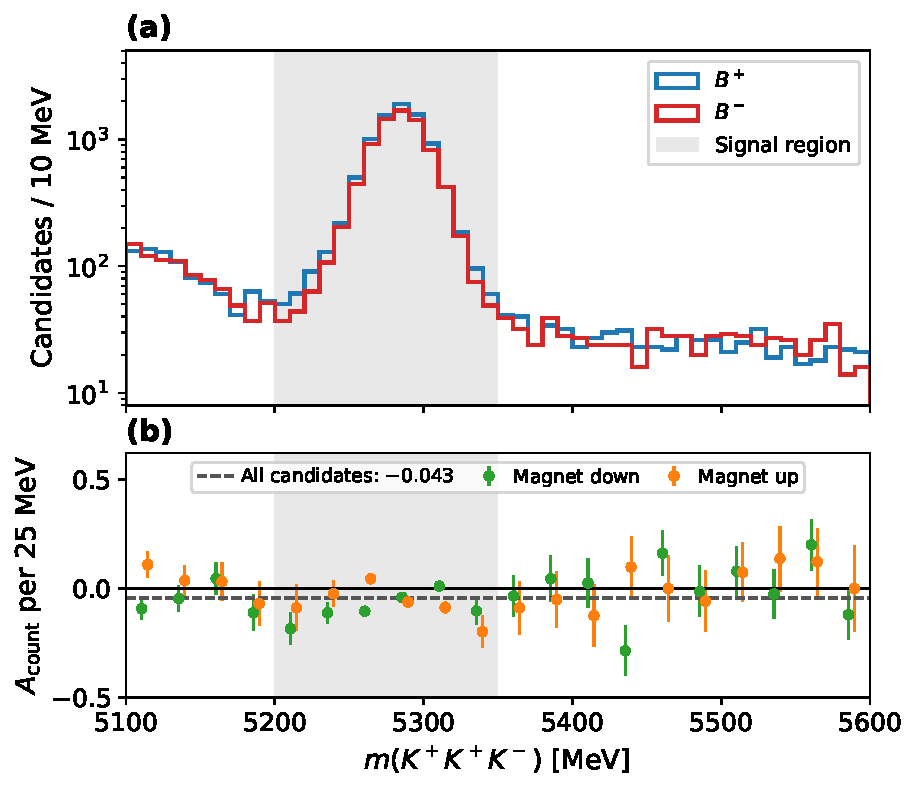
\includegraphics[width=\columnwidth]{figures/mass_spectrum_col.pdf}
\caption{(a) Reconstructed $B\to KKK$ invariant mass in the nominal fit window $[5100,5600]\,\MeV$ for $B^+$ and $B^-$, logarithmic scale; the signal region $[5200,5350]\,\MeV$ is shaded. (b) Counting asymmetry in $25\,\MeV$ bins of the mass for the two magnet polarities, and for all candidates (dashed); the two polarities agree within their uncertainties and the asymmetry is similar in the peak and in the sidebands.}
\label{fig:mass_spectrum}
\end{figure}

\subsection{Cut Flow of the Preselection}
\label{app:cutflow}
\emph{In short: the kaon-identification requirement on the three tracks is by far the most selective.}

\subsection{Candidates Sharing a Track}
\emph{In short: only $42$ candidates of the fit window ($0.2\%$) share a track with another candidate, a negligible effect, and all are kept.}
The files have no event identifier; only $42$ candidates of the fit window ($0.2\%$) share a track with another candidate, a negligible effect, and all are kept.
\subsection{Charge Combinations}
\emph{In short: $H1$ is always the kaon of charge opposite to the $B$ and $H2$, $H3$ the same-sign pair, so the Dalitz variables are the two opposite-sign invariant masses.}
In this dataset only the charge combinations $(+1,-1,-1)$ and $(-1,+1,+1)$ occur for $(H1,H2,H3)$: $H1$ is always the kaon of charge opposite to the $B$, and $H2$, $H3$ are the interchangeable same-sign pair. The Dalitz-plot variables are therefore the invariant masses of the two opposite-sign pairs, $m^2(H1,H2)$ and $m^2(H1,H3)$.

\section{Mass Model and Likelihood}
\label{sec:model}
\label{app:model}
\label{sec:bayes_model}
\emph{In short: a Gaussian signal and a double-exponential background for each charge, with the raw asymmetry $A$ as a parameter of the fit; both inference methods use the same likelihood.}
The mass spectrum of each charge sample is described by a signal-plus-background mixture on the nominal fit window $[5100,5600]\,\MeV$ (Sec.~\ref{sec:data_mass}),
\begin{equation}
f^{\pm}(m)=N_s^{\pm}\,S(m;\mu,\sigma)+N_b^{\pm}\,B^{\pm}(m),
\label{eq:mixture}
\end{equation}
where $S$ is a Gaussian truncated to the window, with mean $\mu$ and width $\sigma$ shared by the two charges, and the background is a double exponential with a shape of its own for each charge,
\[
B^{\pm}(m)=f_{\pm}\,E(m;\lambda_{1}^{\pm})+(1-f_{\pm})\,E(m;\lambda_{2}^{\pm}),
\]
with $E(m;\lambda)\propto e^{-\lambda m}$ a truncated exponential normalized on the window. The steep component ($\lambda_1$) describes the rise of the background towards the lower edge of the window, the slow one ($\lambda_2$) the combinatorial background under and above the peak. The ordering $\lambda_1>\lambda_2$ removes the label-switching symmetry of the mixture. Signal and background yields are split between the charges as
\[
N_s^{\pm}=\tfrac{N_s}{2}(1\mp A),\qquad N_b^{\pm}=\tfrac{N_b}{2}(1\mp A_b),
\]
so that $A=(N_s^--N_s^+)/(N_s^-+N_s^+)$, the raw asymmetry \Araw of Eq.~\eqref{eq:araw}, is itself a parameter of the fit, the parameter of interest (POI, all the others being nuisance parameters), and the background asymmetry $A_b$ is free. The parameter vector has twelve components, $\theta=(N_s,N_b,A,A_b,\mu,\sigma,\lambda_1^{\pm},\lambda_2^{\pm},f_{\pm})$.
Given the data $D=\{(m_i,q_i)\}_{i=1}^{N}$ (mass and charge of each candidate), the extended unbinned likelihood of the two charge samples is
\begin{multline}
\mathcal{L}(D\mid\theta)\propto e^{-(N_s+N_b)}
\prod_{i:\,q_i=+1}\Big[N_s^{+}S(m_i)+N_b^{+}B^{+}(m_i)\Big] \\
\times\prod_{i:\,q_i=-1}\Big[N_s^{-}S(m_i)+N_b^{-}B^{-}(m_i)\Big],
\label{eq:likelihood}
\end{multline}
where $S(m_i)\equiv S(m_i;\mu,\sigma)$. The likelihood is extended (the yields are parameters, hence the Poisson term, Sec.~\ref{app:model}); it is the common ground of the two mass analyses: Sec.~\ref{sec:frequentist} maximizes it and Sec.~\ref{sec:bayesian} multiplies it by a prior. Since both use this model unchanged, any difference between their results can only come from the inference.
\subsection{Extended Likelihood}
\emph{In short: with a Poisson total number of candidates the likelihood is $e^{-(N_s+N_b)}\prod_i[N_s S+N_b B]$ up to a constant, which constrains the yields and $A$ together.}
If the total number of candidates $N$ is Poisson-distributed with mean $\nu=N_s+N_b$ and each candidate is drawn independently from the normalized density $f(m,q)=[N_s S+N_b B]/\nu$, the likelihood of the sample is $\frac{\nu^N e^{-\nu}}{N!}\prod_{i}f(m_i,q_i)=\frac{e^{-\nu}}{N!}\prod_i[N_s S(m_i)+N_b B(m_i)]$. The factor $1/N!$ does not depend on the parameters and is dropped, which gives the extended likelihood of Eq.~\eqref{eq:likelihood}. Unlike the likelihood with a fixed total, it constrains the yields $N_s$ and $N_b$ through $N$ itself, and the asymmetry $A$ is estimated together with them.
\subsection{Extended Likelihood versus a Mixture with Fixed Total}
\emph{In short: the extended form differs from a mixture with fixed total only by the Poisson term of the total yield, which carries no information on $A$; the purity of the signal window is about $96\%$.}
The extended form differs from a mixture of signal and background with a fixed total number of candidates and a signal fraction only through the Poisson term for the total yield, which carries no information on $A$ and does not change its estimate; it is used because the yields of the two charges are the natural parameters of the model. Bayes' theorem applied to the fitted yields gives the probability that a candidate in the signal window $|m-\mu|<2\sigma$ is a signal decay, about $96\%$: a purity, not a property of the single candidate, which depends on the signal fraction of the sample (here $78\%$ of the candidates in the fit window).
\subsection{Label Switching of the Background Components}
\emph{In short: the mixture is invariant under the exchange of the two exponentials, which would give two identical modes; the ordering $\lambda_1>\lambda_2$ removes the symmetry.}
The mixture is invariant under the exchange $(\lambda_1,f)\leftrightarrow(\lambda_2,1-f)$, which would give the posterior two identical modes (label switching); the ordering $\lambda_1>\lambda_2$ removes this symmetry.
\subsection{Minimal Model as a Cross-Check}
\label{sec:bayes_minimal}
\emph{In short: a six-parameter model on a narrower window gives $\Araw=-0.0497$ (68\% CI $[-0.058,-0.041]$), compatible with the nominal result within its uncertainty; it is the model used for the low-statistics comparison.}
Before the nominal model was fixed, the same analysis was carried out with a minimal six-parameter model: a narrower window, $[5150,5450]\,\MeV$, which excludes most of the rising background below the peak, a single exponential background with a shape and a yield shared by the two charges, and the same Gaussian signal. On its $17{,}839$ candidates it gives $\Araw=-0.0497$ (68\% CI $[-0.058,-0.041]$) with $\chi^2/\text{ndof}=127.4/54$, and $-0.0457$ when the background yields of the two charges are left free. Its toy validation, with 500 toy-MC datasets, gives coverage consistent with nominal (0.664 and 0.962 for the 68\% and 95\% intervals). The difference from the nominal result, $0.005$, is driven by the background treatment, as in the systematic study of Sec.~\ref{sec:syst}, and is smaller than the statistical uncertainty.
\FloatBarrier

\section{Frequentist Analysis}
\label{sec:frequentist}
\label{app:freq}
\emph{In short: the likelihood maximized for the two charges together gives $N_s=15{,}328\pm133$ and $\hat A=-0.0441$ with Minos intervals; $A=0$ is rejected at $5.2\sigma$ and the interval has nominal coverage in $1000$ bootstrap replicas.}
The Frequentist analysis estimates \Araw by maximizing the extended unbinned likelihood of Eq.~\eqref{eq:likelihood} with \texttt{iminuit}~\cite{iminuit}; the uncertainty and the test of $A=0$ come from the profile likelihood, the other parameters being nuisance parameters (Secs.~\ref{sec:freq_model}--\ref{sec:freq_ci}).
\subsection{Mass Model and Fit Strategy}
\label{sec:freq_model}
\label{sec:freq_simfit}
The common mass model of Sec.~\ref{sec:model} (Eq.~\eqref{eq:mixture}) was fitted on $[5100,5600]\,\MeV$: a Gaussian signal with mean $\mu$ and width $\sigma$ shared by the two charges and a double-exponential background with shape and yield of its own for each charge, twelve parameters as in the Bayesian fit, through \texttt{iminuit.cost.ExtendedUnbinnedNLL}; the minimization started from an unbinned fit of the sidebands (the window without $[5200,5350]\,\MeV$). The asymmetry was estimated in two ways: in the \emph{simultaneous} fit the two charges share $N_s^\pm=N_s(1\mp A)/2$ and $A$ is a parameter of the likelihood; in the \emph{separate} fits each charge was fitted alone (seven free parameters each) and $\Araw=(N_s^--N_s^+)/(N_s^-+N_s^+)$ was computed from the two yields. They give $-0.0441\pm0.0085$ and $-0.0442\pm0.0087$: sharing $\mu$ and $\sigma$ between a particle and its antiparticle is adequate, and the simultaneous fit, which gives the profile-likelihood interval directly, is the nominal one. It gives $N_s=15{,}328\pm133$ and $N_b=4{,}403\pm82$, against the Bayesian posterior medians $15{,}328\pm133$ and $4404\pm82$ (Sec.~\ref{sec:bayes_posterior}). The shapes were not tuned on this fit, and the alternatives are systematic variants (Sec.~\ref{sec:syst}). The nominal fit has $\chi^2/\mathrm{ndof}=160/88$ ($p=4.8\cdot 10^{-6}$) in $2\times50$ bins of $10\,\MeV$; a single exponential is rejected ($294/92$, $p=5.7\cdot 10^{-23}$)\appref{sec:validation_gof} because the background rises towards the lower edge of the window (Sec.~\ref{sec:data_mass}). The fit of the two charges is shown in Fig.~\ref{fig:freq_jointfit}.

\begin{figure*}[t]
\centering
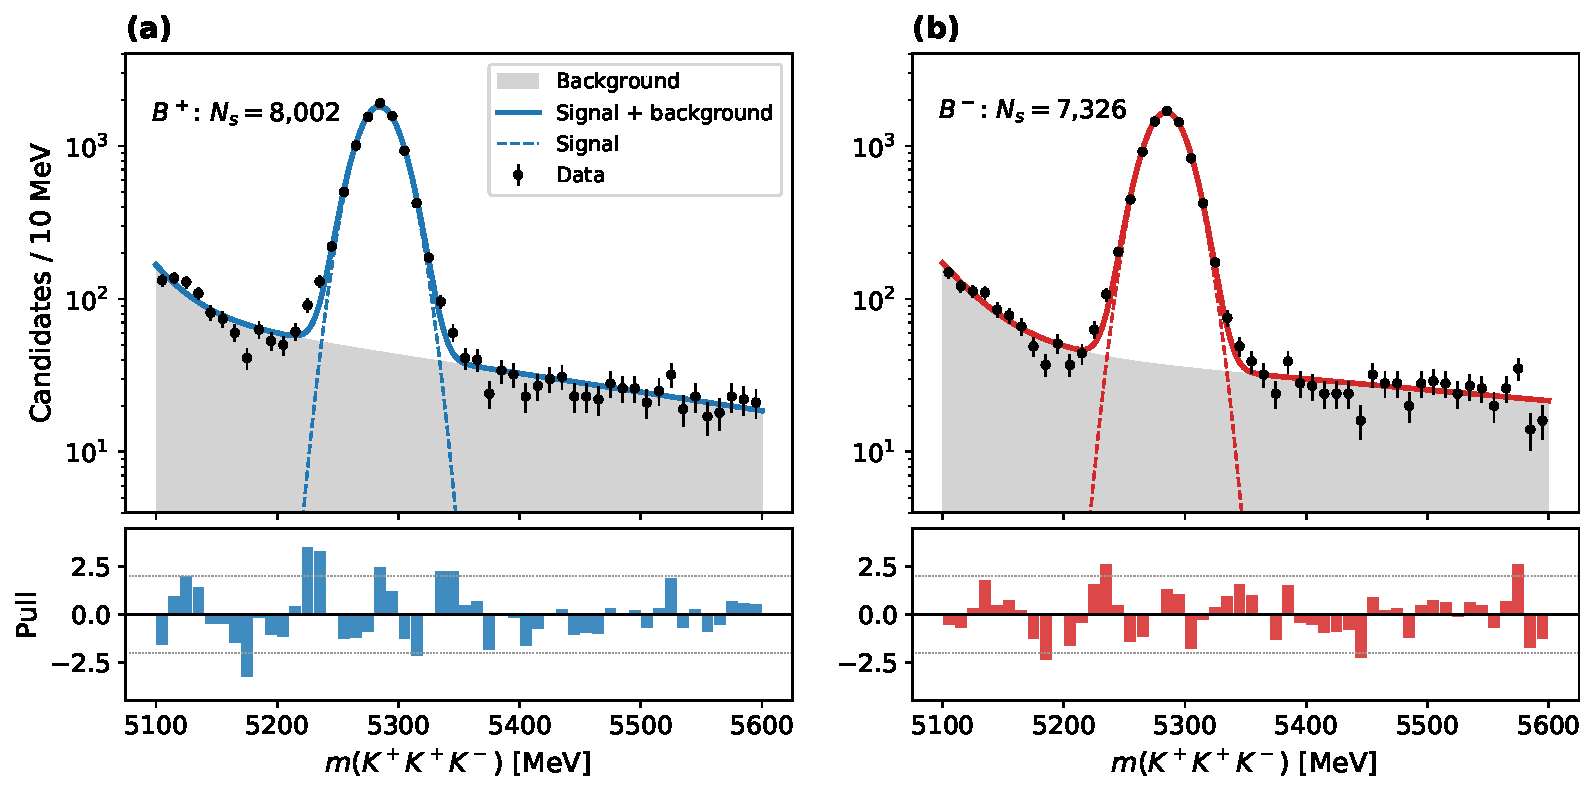
\includegraphics[width=0.95\textwidth]{figures/freq_jointfit.pdf}
\caption{Simultaneous fit of (a) $B^+$ and (b) $B^-$ in $10\,\MeV$ bins, logarithmic scale: data, signal (dashed), double-exponential background (grey) and their sum; below, the pulls $(n_i-\mu_i)/\sqrt{\mu_i}$ of the fit, with the $\pm2$ lines. The fitted signal yields are $8002$ and $7326$.}
\label{fig:freq_jointfit}
\end{figure*}

\subsection{Profile Likelihood and Confidence Interval}
\label{sec:freq_ci}
The maximum-likelihood estimate is $\hat A=-0.0441$ (Hesse uncertainty $0.0085$), with \texttt{MINOS}~\cite{minuit} intervals $68\%$ CI $[-0.0526,-0.0356]$ and $95\%$ CI $[-0.0607,-0.0275]$; the uncertainties are statistical only (the systematic one is in Sec.~\ref{sec:syst}). The profile likelihood ratio $q(A)=-2\log[L(A,\hat{\hat\theta})/L(\hat A,\hat\theta)]$, with the other eleven parameters re-minimized at each $A$ (\texttt{mnprofile}), is shown in Fig.~\ref{fig:freq_profile}; by Wilks' theorem~\cite{wilks} it follows a $\chi^2$ distribution with one degree of freedom at the true value of $A$, so the intervals are the sets $q\leq1$ and $q\leq3.84$. For the null hypothesis, $q(0)\simeq27$, $p=2.05\times10^{-7}$, $5.20\sigma$\appref{sec:appendix_freq}: no asymmetry is rejected, the counterpart of the Savage-Dickey test of Sec.~\ref{sec:bayes_factor} ($A=0$ at $5.2$ posterior standard deviations); the $p$-value is not the probability of $H_0$ and the Bayes factor depends on the prior width, but the conclusion is the same. The result agrees with the Bayesian one (Sec.~\ref{sec:bayes_posterior}: $-0.0443$, $68\%$ CI $[-0.0528,-0.0358]$), as expected with flat priors and $\sim2\times10^4$ events.

\begin{figure}[h]
\centering
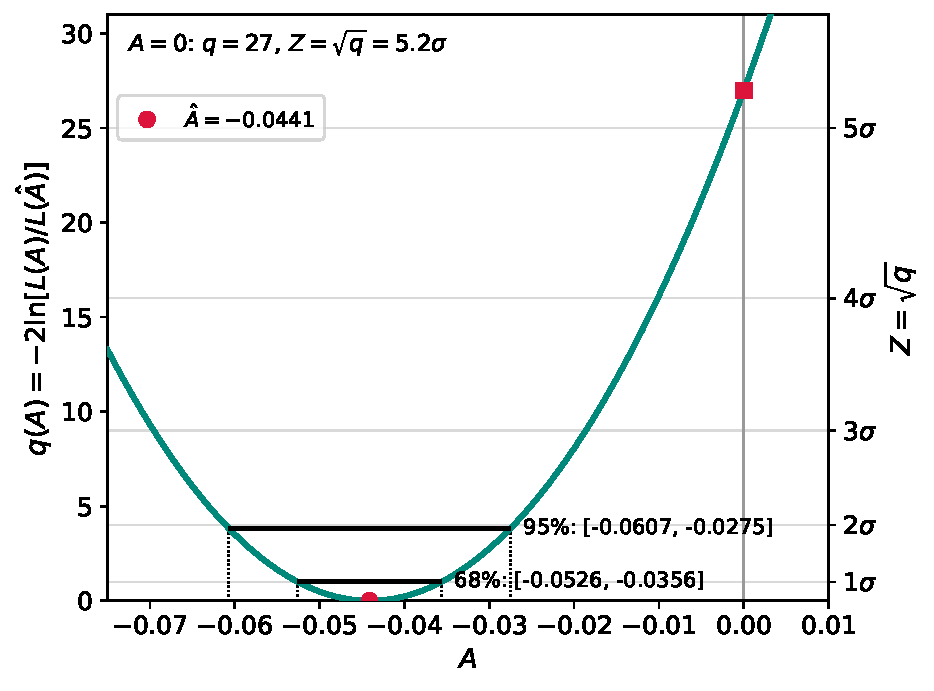
\includegraphics[width=\columnwidth]{figures/freq_profile.pdf}
\caption{Profile likelihood ratio $q(A)$ of the simultaneous fit, with the other eleven parameters re-minimized at each $A$ (right axis: $Z=\sqrt q$). The horizontal segments are the $68\%$ and $95\%$ Minos intervals ($q\leq1$, $q\leq3.84$); at $A=0$, $q\simeq27$, i.e. $5.2\sigma$.}
\label{fig:freq_profile}
\end{figure}

\subsection{Coverage of the Wilks Intervals}
\label{sec:freq_coverage}
Wilks' theorem is asymptotic, so the coverage was checked on the data with $1000$ bootstrap replicas of the $19{,}731$ candidates, refitting the nominal model on each (non-converged fits discarded); with $A_{\mathrm{true}}=-0.0441$, the $68\%$ interval of a replica contains it if and only if $q(A_{\mathrm{true}})\leq1$. The fraction is $68.4\pm1.5\%$ against $68.3\%$ nominal (Fig.~\ref{fig:freq_toys}). It agrees with the toy-MC check of the Bayesian interval ($65.0\pm3.3\%$, $200$ experiments)\appref{sec:bayes_toymc}; the two checks are not equivalent, since the Bayesian pseudo-datasets come from the fitted model (a closure test) while the replicas are resampled from the data and carry the features that the model does not describe, such as the signal tails\appref{sec:bayes_gof}.

\begin{figure}[h]
\centering
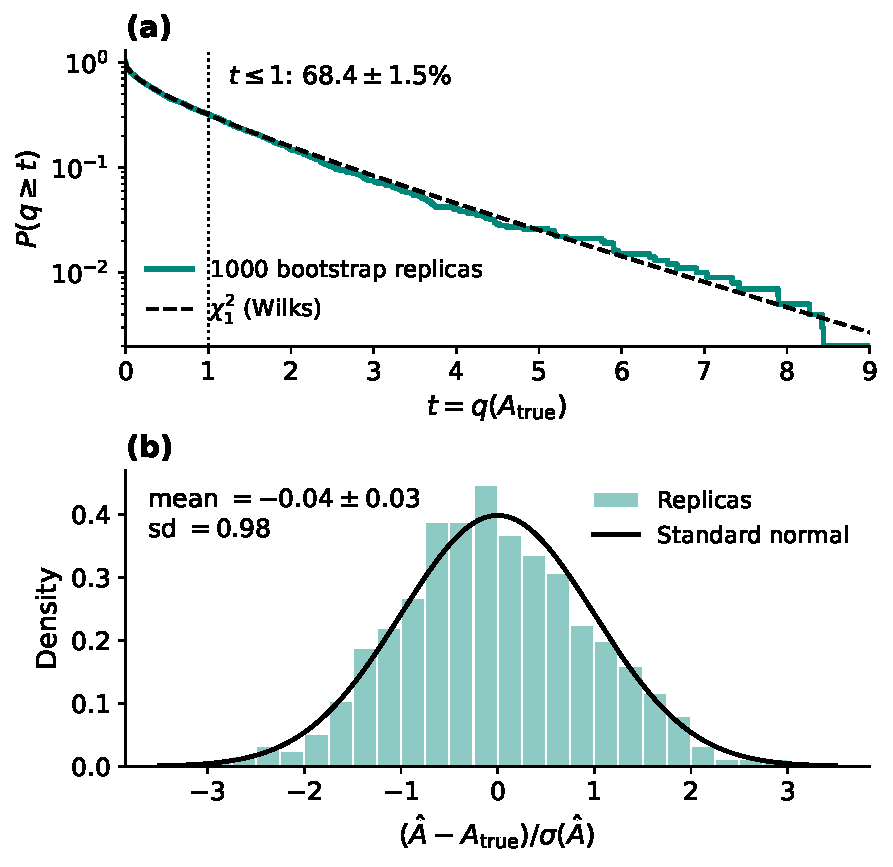
\includegraphics[width=\columnwidth]{figures/short_coverage.pdf}
\caption{Coverage check with $1000$ bootstrap replicas of the data. (a) Survival function of $t=q(A_{\mathrm{true}})$ against the $\chi^2_1$ distribution expected from Wilks' theorem; the dotted line is the $68.3\%$ limit ($t=1$). (b) Pulls $(\hat A-A_{\mathrm{true}})/\sigma(\hat A)$ of the replicas against a standard normal.}
\label{fig:freq_toys}
\end{figure}

\subsection{Hesse Uncertainties, Test of $A=0$ and Significance}
\label{sec:appendix_freq}
\emph{In short: the Hesse matrix is the inverse of the Fisher information, the test statistic is the profile likelihood ratio, and the significance is $Z=\sqrt{q(0)}$.}
\paragraph{Hesse uncertainties.}
For $n$ independent candidates the likelihood contains the information on the parameters $\theta$ through the Fisher information matrix, $I_{ij}=-E\big[\partial^2\ln L/\partial\theta_i\partial\theta_j\big]$. The information inequality (minimum variance bound) states that the variance of an estimator cannot be smaller than the inverse of $I$ (for an unbiased one), and the maximum-likelihood estimate reaches the bound asymptotically, where it is also unbiased and Gaussian~\cite{cowan}. The covariance matrix of the fit is therefore $V\simeq I^{-1}$ evaluated at the best-fit point, with the second derivatives of $-\ln L$ computed numerically: this is the Hesse matrix of \texttt{iminuit}, and $\sigma(A)=0.0085$ is the square root of the diagonal element of $V$ for $A$, which includes the effect of the eleven nuisance parameters. It assumes that $-\ln L$ is parabolic around the minimum. The Minos intervals do not: they follow the profile likelihood on each side of the minimum, and their agreement with the Hesse error ($-0.0085$, $+0.0085$) shows that the parabola is a good description here.
\paragraph{Test of $A=0$.}
The null hypothesis $H_0$: $A=0$ is tested against the alternative $H_1$: $A$ free, the other parameters being free in both. The test statistic is the profile likelihood ratio,
$q(0)=-2\ln\big[L(0,\hat{\hat\theta})/L(\hat A,\hat\theta)\big]=2\Delta\mathrm{NLL}$ (NLL: negative log-likelihood), large when the data disfavor $H_0$. For two simple hypotheses the likelihood ratio is the most powerful test of a given size, i.e.\ the one with the highest probability of rejecting $H_0$ when $H_1$ is true (Neyman-Pearson lemma~\cite{neyman_pearson}); the profile likelihood ratio is its extension to hypotheses with unspecified parameters, with no optimality guarantee in general. By Wilks' theorem~\cite{wilks}, under $H_0$ the statistic follows a $\chi^2$ distribution with one degree of freedom, the number of parameters fixed by $H_0$, whatever the number of nuisance parameters, so the $p$-value is $P(\chi^2_1\geq q_{\mathrm{obs}})$; this is the probability, under $H_0$, of a result at least as discrepant as the data, not the probability of $H_0$.
\paragraph{Significance.}
A $\chi^2_1$ variable is the square of a standard normal one, so $p=P(|N|\geq\sqrt{q})$ and the significance quoted is $Z=\sqrt{q(0)}$ ($q\simeq27$, $p=2.05\times10^{-7}$, $Z=5.20$). This is a two-sided convention: the one-sided one, $Z=\Phi^{-1}(1-p)$, applied to the same $p$ would give $5.06$. For a parabolic likelihood $\sqrt{q}$ coincides with the Hesse significance $|\hat A|/\sigma(A)=5.19$.
\subsection{Neyman Construction and Dependence on the Momentum}
\label{sec:checks_belt}
\emph{In short: inverting the test of $A_{\mathrm{true}}$ with toy-MC experiments gives the same interval as the likelihood ratio, and $\Araw$ does not depend on the momentum of the $B$.}
The confidence interval is, by definition, the set of $A_{\mathrm{true}}$ not rejected by the data. It was constructed directly (Fig.~\ref{fig:checks_belt}): for $11$ values of $A_{\mathrm{true}}$ between $-0.1$ and $0$, $300$ toy-MC experiments give the central $68\%$ and $95\%$ ranges of $\hat A$ (the belt), and the interval is the set of $A_{\mathrm{true}}$ whose $68\%$ range contains the observed $\hat A=-0.0441$: $[-0.0528,-0.0351]$, against $[-0.0526,-0.0356]$ from the profile likelihood (Minos), which is the content of Wilks' theorem for this problem.

\begin{figure}[h]
\centering
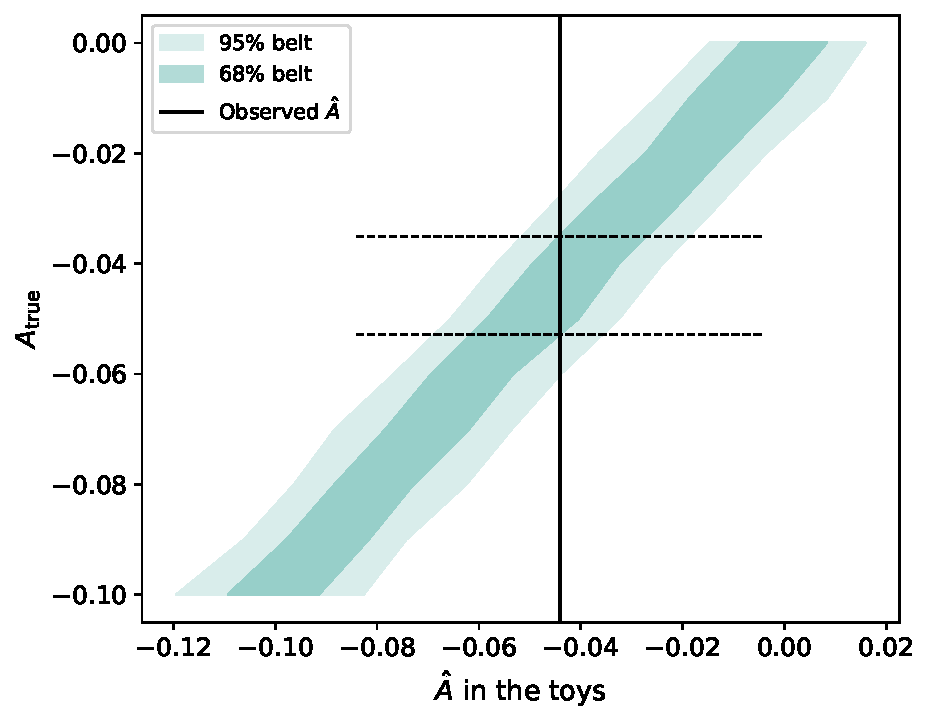
\includegraphics[width=\columnwidth]{figures/validation_neyman_belt.pdf}
\caption{Confidence belt of $\hat A$ from toy-MC experiments (central $68\%$ and $95\%$ ranges) as a function of $A_{\mathrm{true}}$; the vertical line is the observed $\hat A$ and the dashed lines the resulting $68\%$ interval.}
\label{fig:checks_belt}
\end{figure}

The detection asymmetry of kaons depends on their momentum; as a direct check, the joint fit was repeated in three bins with equal numbers of candidates of the transverse momentum $p_T$ and of the momentum $p$ of the $B$ candidate (Table~\ref{tab:checks_momentum}): the three values are compatible with the global one, with a largest deviation of $1.4\sigma$.

\begin{table}[h]
\centering
\begin{tabular}{lccc}
\toprule
Bin & range [GeV] & $n$ & $\Araw$ \\
\midrule
$p_T$, 1 & $1.0$--$4.7$ & $6577$ & $-0.0563\pm0.0169$ \\
$p_T$, 2 & $4.7$--$8.2$ & $6577$ & $-0.0362\pm0.0141$ \\
$p_T$, 3 & $8.2$--$30.5$ & $6577$ & $-0.0452\pm0.0134$ \\
$p$, 1 & $26.7$--$78.1$ & $6577$ & $-0.0391\pm0.0139$ \\
$p$, 2 & $78.1$--$110.1$ & $6577$ & $-0.0475\pm0.0149$ \\
$p$, 3 & $110.1$--$288.5$ & $6577$ & $-0.0478\pm0.0153$ \\
\bottomrule
\end{tabular}
\caption{$\Araw$ (joint Frequentist fit) in terciles of the transverse momentum and of the momentum of the $B$ candidate.}
\label{tab:checks_momentum}
\end{table}

The values of Table~\ref{tab:checks_momentum} are plotted in Fig.~\ref{fig:momentum_terciles} against the global result: no trend with $p_T$ or $p$ is visible.

\begin{figure*}[t]
\centering
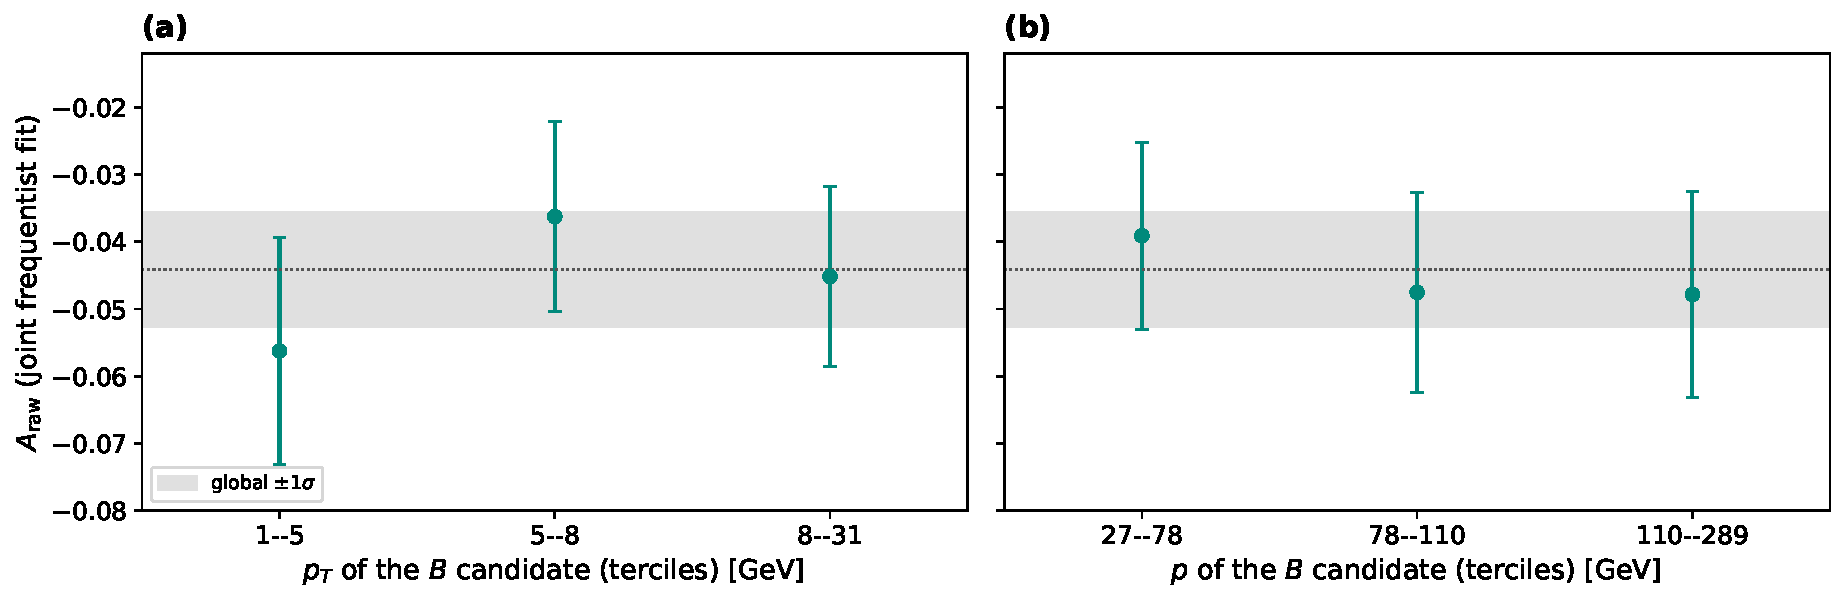
\includegraphics[width=0.85\textwidth]{figures/momentum_terciles.pdf}
\caption{$\Araw$ (joint Frequentist fit) in terciles of (a) the transverse momentum and (b) the momentum of the $B$ candidate, with the global value and its $\pm1\sigma$ band; each bin has $6577$ candidates.}
\label{fig:momentum_terciles}
\end{figure*}

\subsection{Uncertainties of the Twelve Parameters by Three Methods}
\label{sec:checks_covariance}
\emph{In short: the inverse of the Fisher information (Hesse), the bootstrap of the data and the posterior give the same standard deviations for $A$, $A_b$, $\mu$ and $\sigma$; the bootstrap differs for the two yields, because it keeps the total number of candidates fixed, and for the steep slope $\lambda_1^+$, which is weakly constrained.}
The covariance of the fit parameters was estimated in three ways (Table~\ref{tab:checks_covariance}): the inverse of the matrix of second derivatives of $-\ln L$ at the minimum (Hesse), $300$ bootstrap replicas of the data, each refitted, and the posterior sample. The posterior agrees with Hesse to $10\%$ for all the parameters, and the bootstrap does for $A$, $A_b$, $\mu$, $\sigma$ and the other shape parameters. The exceptions of the bootstrap are the steep slope of the $B^+$ background, $\lambda_1^+$ ($0.0057$ against $0.0077$, a weakly constrained and non-parabolic direction, Sec.~\ref{sec:checks_multistart}), and the signal and background yields, $\sigma(N_s)=133$ (Hesse) and $72$ (bootstrap): a resampling of $N$ candidates keeps the total yield fixed, which the extended likelihood does not, and the yields of the bootstrap show the anticorrelated fluctuation of the binomial split; the asymmetry $A$ is not affected. The correlation between $A$ and $A_b$ is $-0.16$, $-0.17$ and $-0.17$ in the three methods.

\begin{table}[h]
\centering
\begin{tabular}{lccc}
\toprule
Parameter & Hesse & Bootstrap & Posterior \\
\midrule
$A$ & $0.0085$ & $0.0085$ & $0.0085$ \\
$A_b$ & $0.0177$ & $0.0183$ & $0.0176$ \\
$N_s$ & $133$ & $72$ & $133$ \\
$N_b$ & $82$ & $72$ & $82$ \\
$\mu$ [MeV] & $0.159$ & $0.159$ & $0.161$ \\
$\sigma$ [MeV] & $0.141$ & $0.150$ & $0.138$ \\
$\lambda_1^+$ & $0.0077$ & $0.0057$ & $0.0078$ \\
$\lambda_2^+$ & $0.00028$ & $0.00030$ & $0.00029$ \\
$f_+$ & $0.028$ & $0.029$ & $0.030$ \\
$\lambda_1^-$ & $0.0047$ & $0.0043$ & $0.0047$ \\
$\lambda_2^-$ & $0.00040$ & $0.00038$ & $0.00039$ \\
$f_-$ & $0.039$ & $0.036$ & $0.037$ \\
\bottomrule
\end{tabular}
\caption{Standard deviation of the parameters of the nominal fit from the Hesse matrix, from the bootstrap of the data and from the posterior.}
\label{tab:checks_covariance}
\end{table}

Figure~\ref{fig:uncertainties_12} shows the same comparison as the ratio to the Hesse uncertainty. The posterior agrees with Hesse within $10\%$ for all parameters; the bootstrap does too, except for the yields (the bootstrap of the data keeps the total number of candidates fixed, which removes the Poisson fluctuation of $N_s$) and $\lambda_1^+$.

\begin{figure*}[t]
\centering
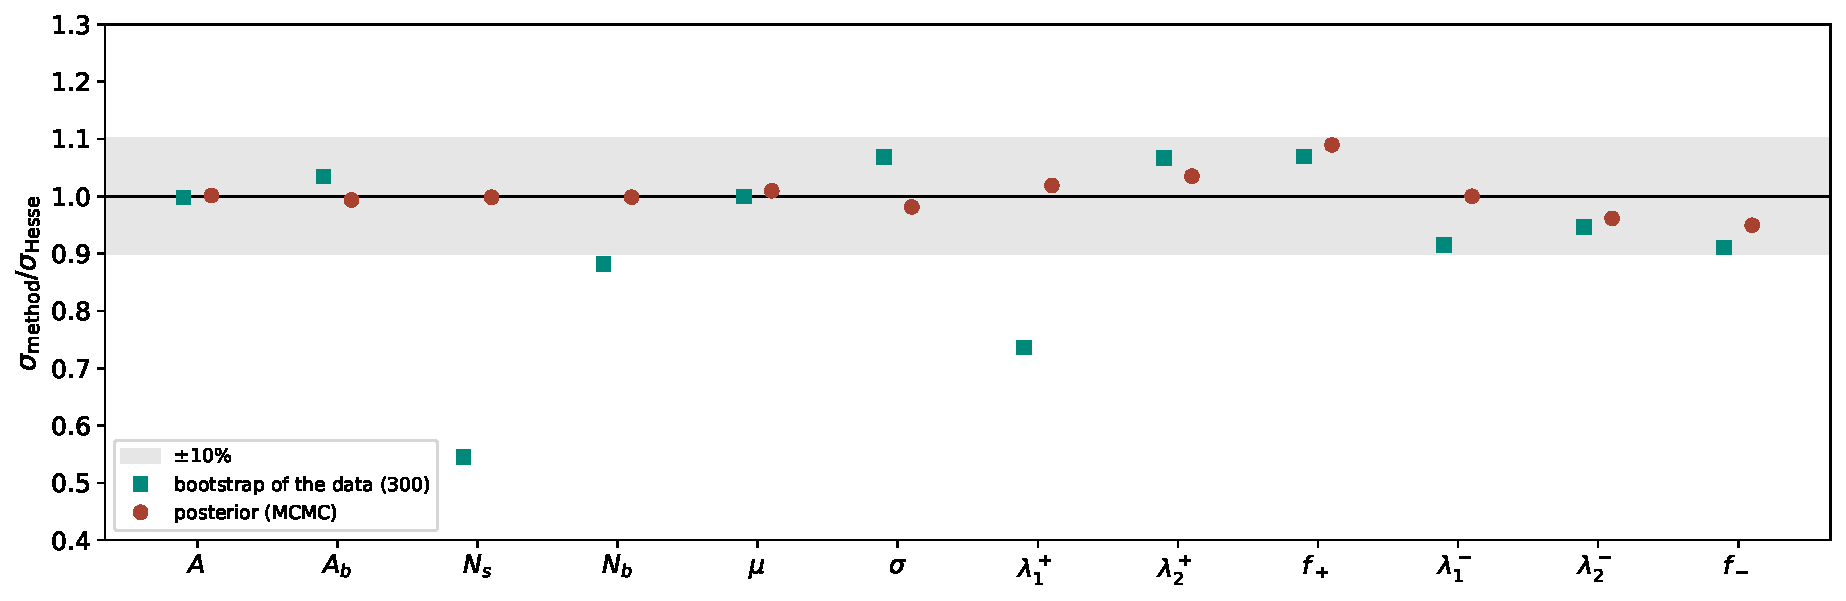
\includegraphics[width=0.85\textwidth]{figures/uncertainties_12.pdf}
\caption{Standard deviation of the twelve parameters of the nominal fit from the bootstrap of the data ($300$ replicas) and from the posterior, divided by the Hesse uncertainty; the band is $\pm10\%$.}
\label{fig:uncertainties_12}
\end{figure*}

\subsection{Starting Values and Weakly Constrained Parameters}
\label{sec:checks_multistart}
\emph{In short: $29$ of $30$ fits from random starting points reach the same minimum; the steep-background fraction is the weakly constrained direction, as the long chain of the Bayesian fit already showed.}
The nominal fit was repeated from $30$ starting points drawn at random (yields and slopes multiplied by a log-normal factor of width $0.5$, the fractions uniform, the asymmetry uniform in $(-0.2,0.2)$): $29$ reach the minimum of the nominal fit ($\hat A=-0.0441$); the remaining one stops in a local minimum $96$ units of $-2\ln L$ above, at $\hat A=-0.052$, which would be rejected by comparing the likelihood values. The profile likelihood of the fraction of the steep component for $B^+$ (the parameter whose chain mixes slowly in the narrow window, Sec.~\ref{sec:bayes_gof}) is asymmetric: $q(f_+)=1$ at $0.085$ and $0.140$ around the best value $0.112$, with a longer tail towards large fractions where the two exponentials exchange their roles. The uncertainty of $A$ does not depend on it (correlation below $0.1$).
\FloatBarrier

\section{Bayesian Analysis}
\label{sec:bayesian}
\label{app:ext_bayes}
\emph{In short: the same likelihood with uniform priors, sampled with MCMC: $\Araw=-0.0443$ ($68\%$ interval $[-0.0528,-0.0358]$) with converged chains; the Bayes factor of $A=0$, $BF_{10}\approx9\times10^3$, depends on the prior width.}
The Bayesian analysis takes the likelihood of Sec.~\ref{sec:model} as it is and adds only a prior and a sampler; it changes the question asked of the data, not the model.
\subsection{Priors and Posterior}
\label{sec:bayes_prior}
\emph{In short: uniform bounded priors on twelve parameters; with $\sim2\times10^4$ candidates the posterior is dominated by the likelihood.}
Bayes' theorem combines the likelihood of Eq.~\eqref{eq:likelihood} (Sec.~\ref{sec:model}) with a prior $\pi(\theta)$ into the posterior
\begin{equation}
p(\theta\mid D)=\frac{\mathcal{L}(D\mid\theta)\,\pi(\theta)}{p(D)},
\label{eq:bayes}
\end{equation}
The priors are uniform, with independent ranges except for the ordering of the background slopes: $N_s,N_b\in(0,5N)$ with $N=19{,}731$, $A,A_b\in(-1,1)$, $\mu\in(5260,5310)\,\MeV$, $\sigma\in(3,40)\,\MeV$, $\lambda_1^{\pm}\in(10^{-5},0.1)\,\MeV^{-1}$, $\lambda_2^{\pm}\in(10^{-5},\lambda_1^{\pm})$, $f_{\pm}\in(0,1)$. The prior density is therefore a constant on the allowed region $\Theta$,
\begin{equation}
\pi(\theta)\propto\mathbf{1}\left[\theta\in\Theta\right],
\label{eq:prior}
\end{equation}
and inside it the posterior is proportional to the likelihood. With $\sim$$2\times10^4$ events the posterior is dominated by the likelihood, as the prior-sensitivity check confirms for $A$. The evidence $p(D)$ is a constant: the MCMC samples $\mathcal{L}\,\pi$ without it, and the Savage-Dickey ratio of Sec.~\ref{sec:bayes_factor} avoids it as well; the marginal posterior of $A$ is the histogram of the $A$ component of the chain.
\subsection{MCMC Sampling and Convergence Diagnostics}
\label{sec:bayes_mcmc}
\emph{In short: 32 walkers for $25{,}000$ steps; the chain is at least $113$ autocorrelation times long for every parameter and independent runs from dispersed starting points agree.}
The posterior was sampled with the affine-invariant ensemble sampler of Goodman and Weare~\cite{goodman_weare} as implemented in \texttt{emcee}~\cite{emcee} (Sec.~\ref{app:theory}): 32 walkers started around the maximum of the posterior, $25{,}000$ steps with the first $1/6$ discarded as burn-in ($6.7\times10^5$ samples, acceptance $0.38$). The integrated autocorrelation time is $\tau\in[147,183]$ steps, so the chain is $N/\tau\geq113$ autocorrelation times long for every parameter, above the threshold of $50$~\cite{emcee} ($\gtrsim3600$ effectively independent samples). Two runs started uniformly over the whole prior box converge to the same single mode ($\Araw=-0.0446$ and $-0.0442$).
\subsection{Posterior Results and Credible Intervals}
\label{sec:bayes_posterior}
\emph{In short: $\Araw=-0.0443$, 68\% credible interval $[-0.0528,-0.0358]$ and 95\% $[-0.0608,-0.0276]$; the posterior is Gaussian.}

Figure~\ref{fig:bayes_fit} compares the nominal model with the data of the two charges: it follows the spectrum over two orders of magnitude, and the pulls show signal tails heavier than a Gaussian, whose effect on $\Araw$ is negligible (Sec.~\ref{sec:bayes_gof}). The marginal posterior on the raw asymmetry gives (median and equal-tailed credible intervals, CI)
\begin{gather*}
\Araw = -0.0443, \\
68\%~\text{CI}~[-0.0528,-0.0358], \\ 95\%~\text{CI}~[-0.0608,-0.0276].
\end{gather*}
The posterior is very close to Gaussian (standard deviation $0.0085$), so equal-tailed and highest-posterior-density intervals coincide; with uniform priors its mode, $-0.0441$, is the maximum-likelihood estimate and the result can be compared directly with the Frequentist fit (Secs.~\ref{sec:frequentist} and~\ref{sec:appendix_freq}). The other physics parameters (Fig.~\ref{fig:bayes_corner}) are $N_s=15{,}328\pm133$, $N_b=4404\pm82$, $A_b=-0.040\pm0.018$, $\mu=5284.39\pm0.16\,\MeV$ and $\sigma=18.00\pm0.14\,\MeV$. $A$ is almost uncorrelated with them, which is why profiling (Frequentist) and marginalizing (Bayesian) the nuisance parameters give the same result; the largest correlation, $-0.17$, is with $A_b$: conditioning on $A_b=0$ moves $A$ to $-0.0475$, as the fit with a charge-symmetric background does ($-0.0471$, Sec.~\ref{sec:syst}).

\begin{figure*}[!t]
\centering
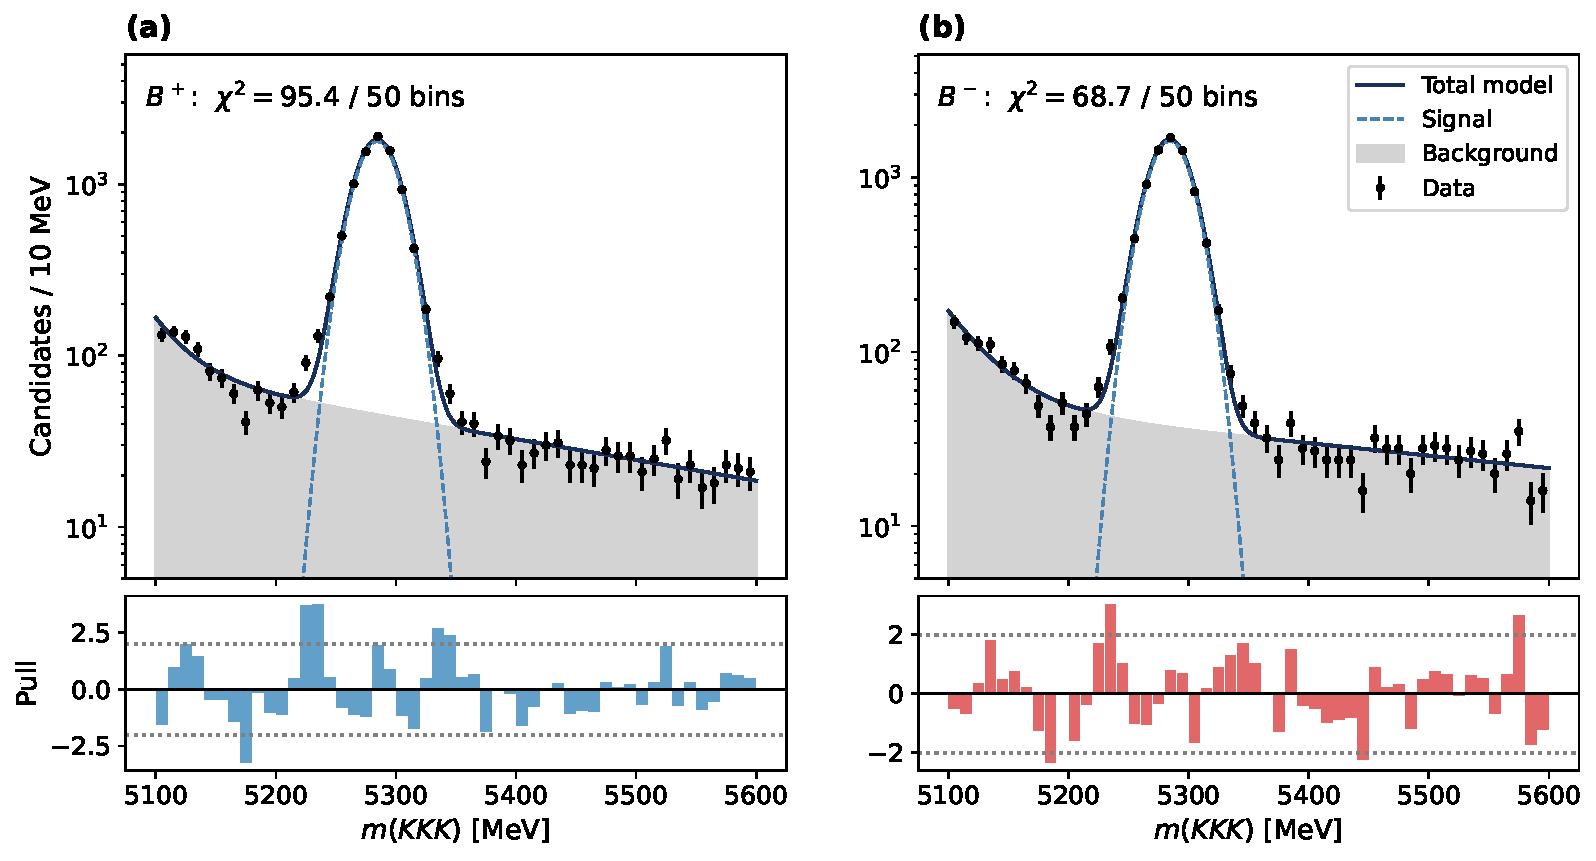
\includegraphics[width=0.8\textwidth]{figures/bayes_nominal_mass_fit.pdf}
\caption{Mass distributions of (a) $B^+$ and (b) $B^-$ candidates with the nominal model (posterior medians, logarithmic scale): total, signal and background components. Bottom: pulls, $(\text{obs}-\text{exp})/\sqrt{\text{exp}}$.}
\label{fig:bayes_fit}
\end{figure*}

\begin{figure*}[t]
\centering
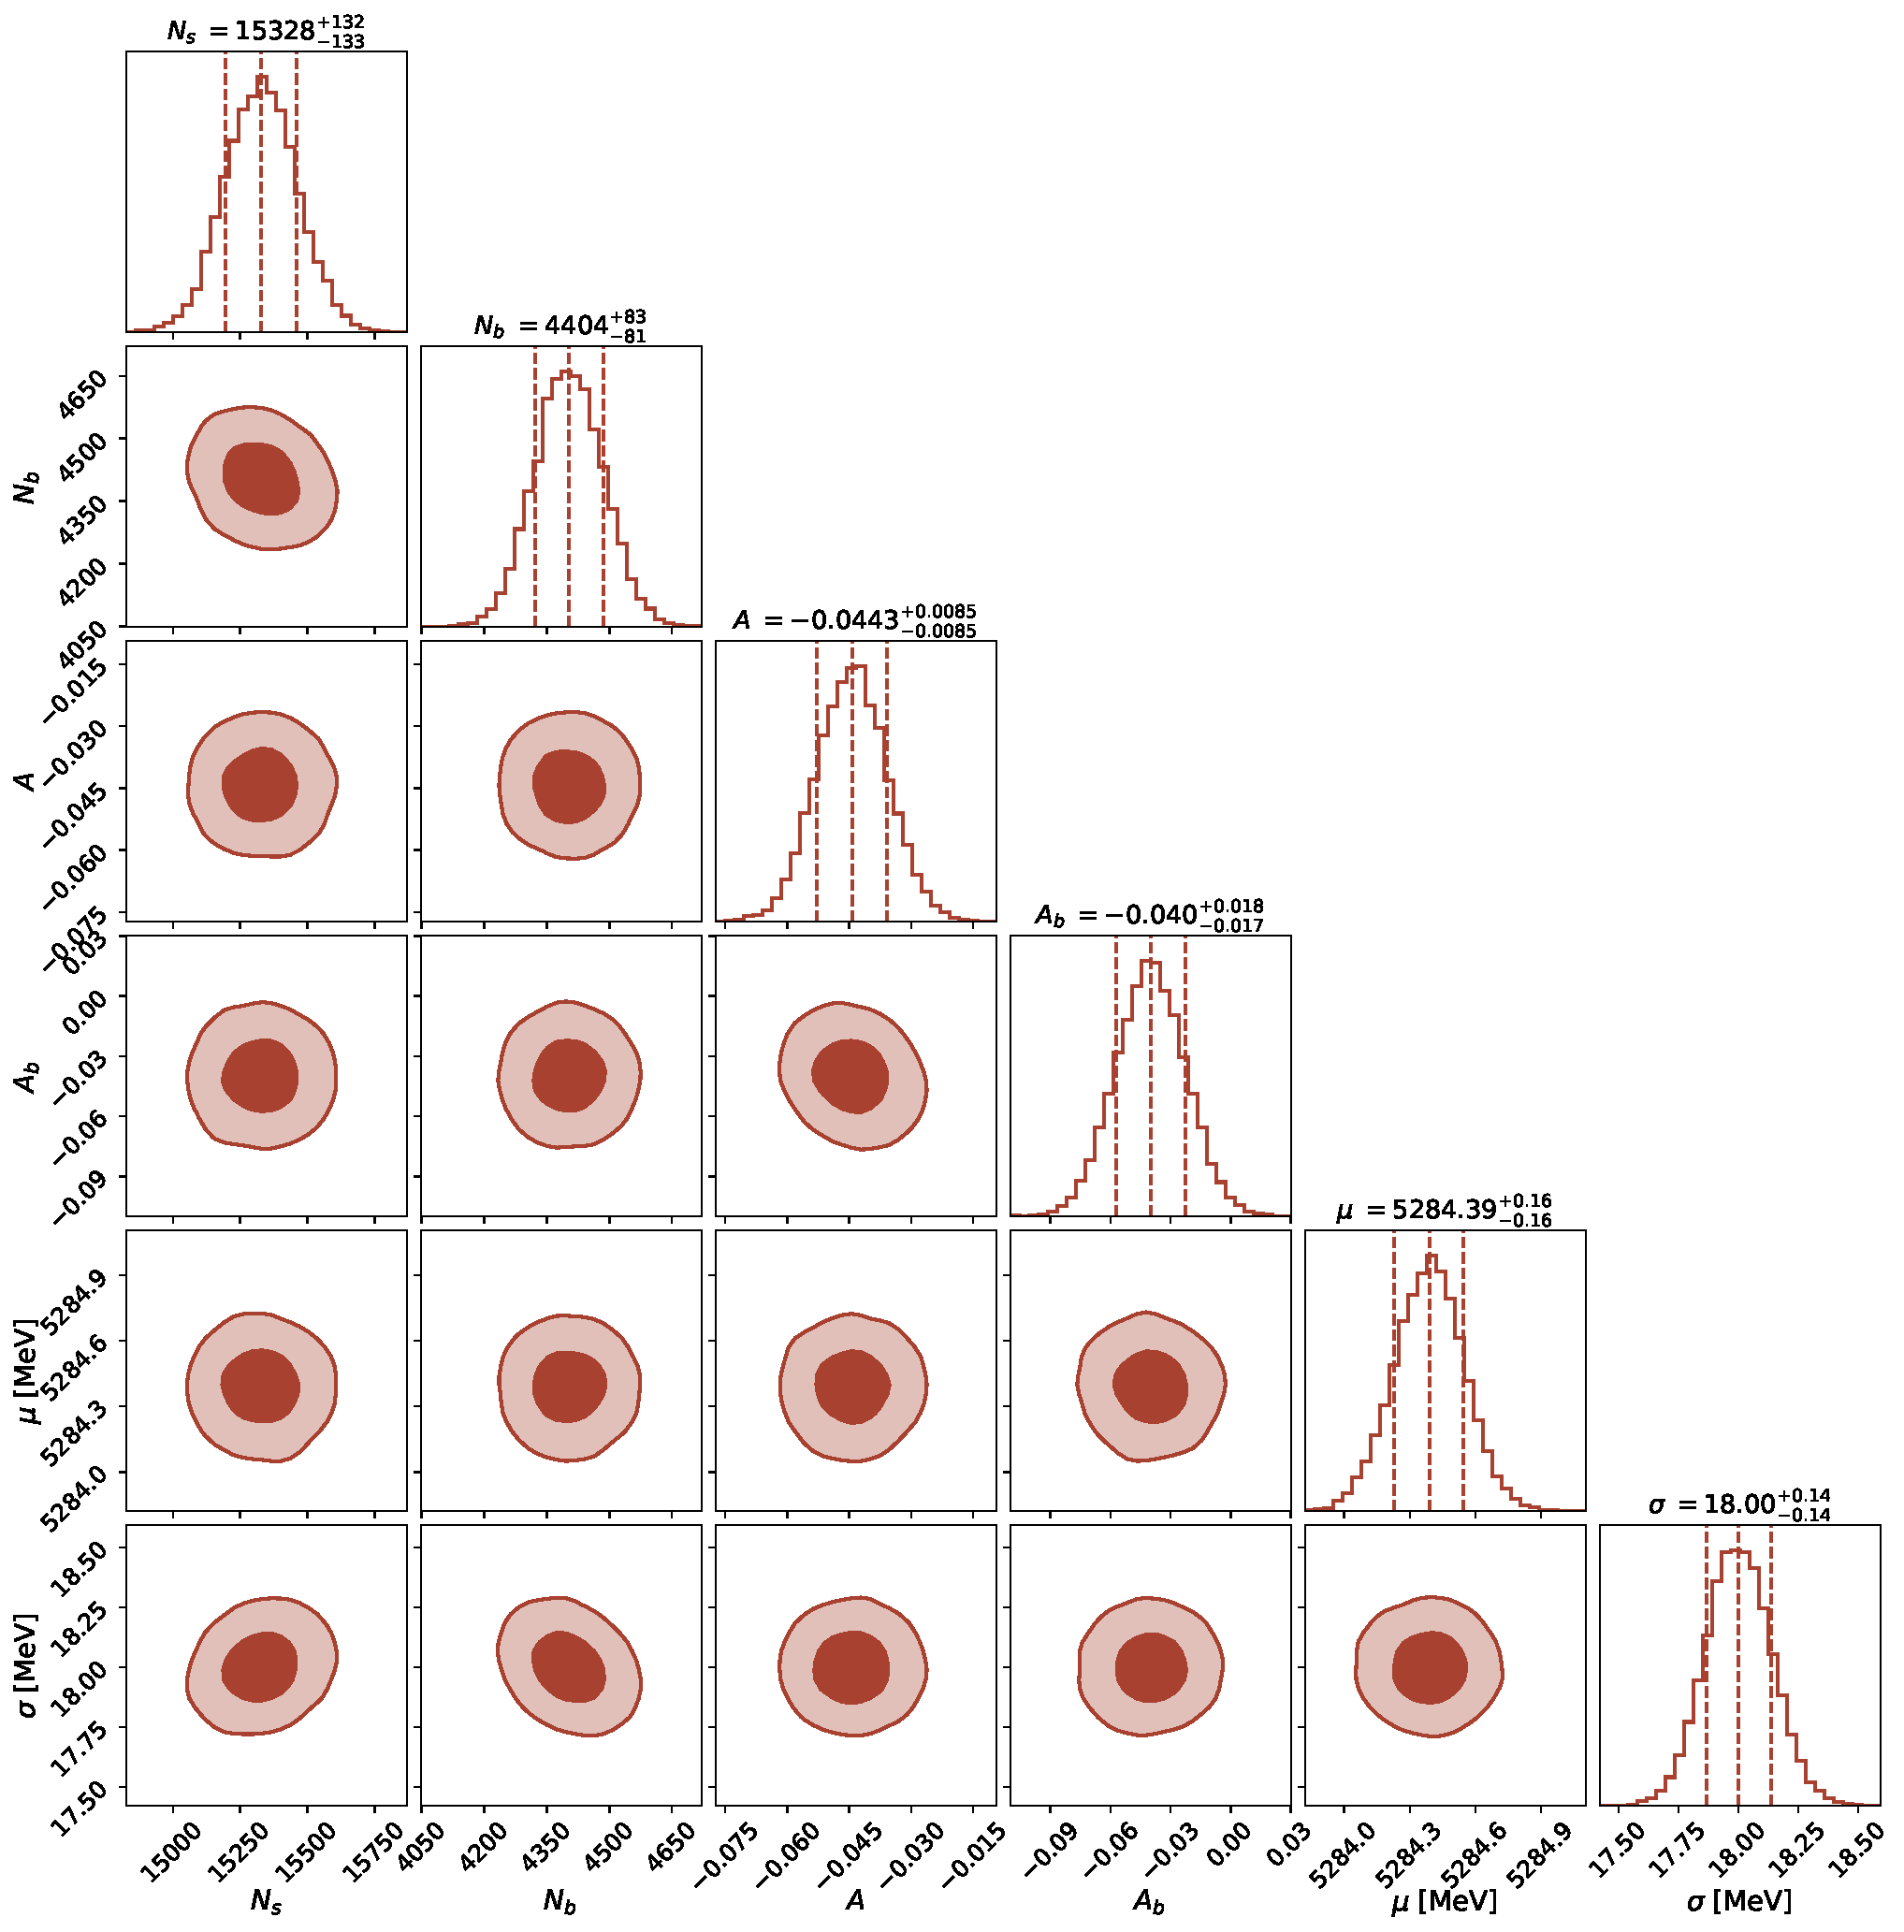
\includegraphics[width=0.55\textwidth]{figures/bayes_nominal_corner.pdf}
\caption{Posterior of the six physics parameters of the nominal fit (the six background-shape parameters are marginalized). Diagonal: marginal posteriors with the 16th, 50th and 84th percentiles (dashed lines and titles). Off-diagonal: 2D marginals, contours enclosing the regions of the $1\sigma$ and $2\sigma$ levels of a 2D Gaussian ($39\%$ and $86\%$).}
\label{fig:bayes_corner}
\end{figure*}

\subsection{Bayes Factors}
\label{sec:bayes_factor}
\emph{In short: decisive evidence against $A=0$ (Bayes factor $BF_{10}\approx9\times10^3$); the evidence for a background asymmetry is not significant, and depends on the prior width.}
The Bayes factor compares two hypotheses through their evidences, $BF_{10}=P(D\mid H_1)/P(D\mid H_0)$, and requires proper priors. For the nested hypothesis $H_0$: $A=0$ against $H_1$: $A$ free, with shared priors on the other parameters, it reduces to the Savage-Dickey ratio~\cite{dickey1971} (Sec.~\ref{sec:appendix_freq}),
\[
BF_{01} = \frac{p(A=0\mid D)}{\pi(A=0)}, \qquad \pi(A=0)=\tfrac12 .
\]
$A=0$ lies $5.2$ posterior standard deviations from the median, where the chain has essentially no samples, so $p(A=0\mid D)$ was taken from the Gaussian approximation of the marginal posterior: $BF_{01}\approx1.1\times10^{-4}$ ($BF_{10}\approx9\times10^{3}$), decisive evidence against $A=0$ on Jeffreys' scale~\cite{jeffreys}. The value scales with the prior width (Ockham factor): with $A\in(-0.3,0.3)$, $BF_{01}$ drops by a factor $3.3$ and the conclusion is unchanged (Fig.~\ref{fig:checks_bf}; the Savage-Dickey densities are in Fig.~\ref{fig:bayes_sd}, further checks in Sec.~\ref{sec:checks_profile}).

\begin{figure}[h]
\centering
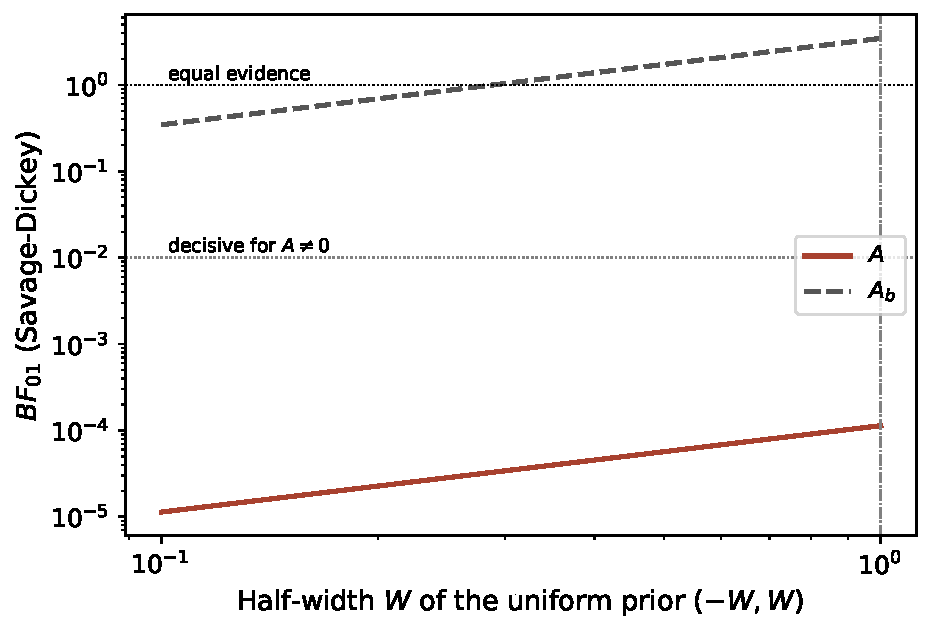
\includegraphics[width=\columnwidth]{figures/validation_bf_prior_width.pdf}
\caption{$BF_{01}$ of $A=0$ and of $A_b=0$ as a function of the half-width $W$ of the uniform prior $(-W,W)$ (Gaussian approximation of the posterior, Savage-Dickey). The vertical line marks the nominal prior.}
\label{fig:checks_bf}
\end{figure}

\begin{figure*}[!t]
\centering
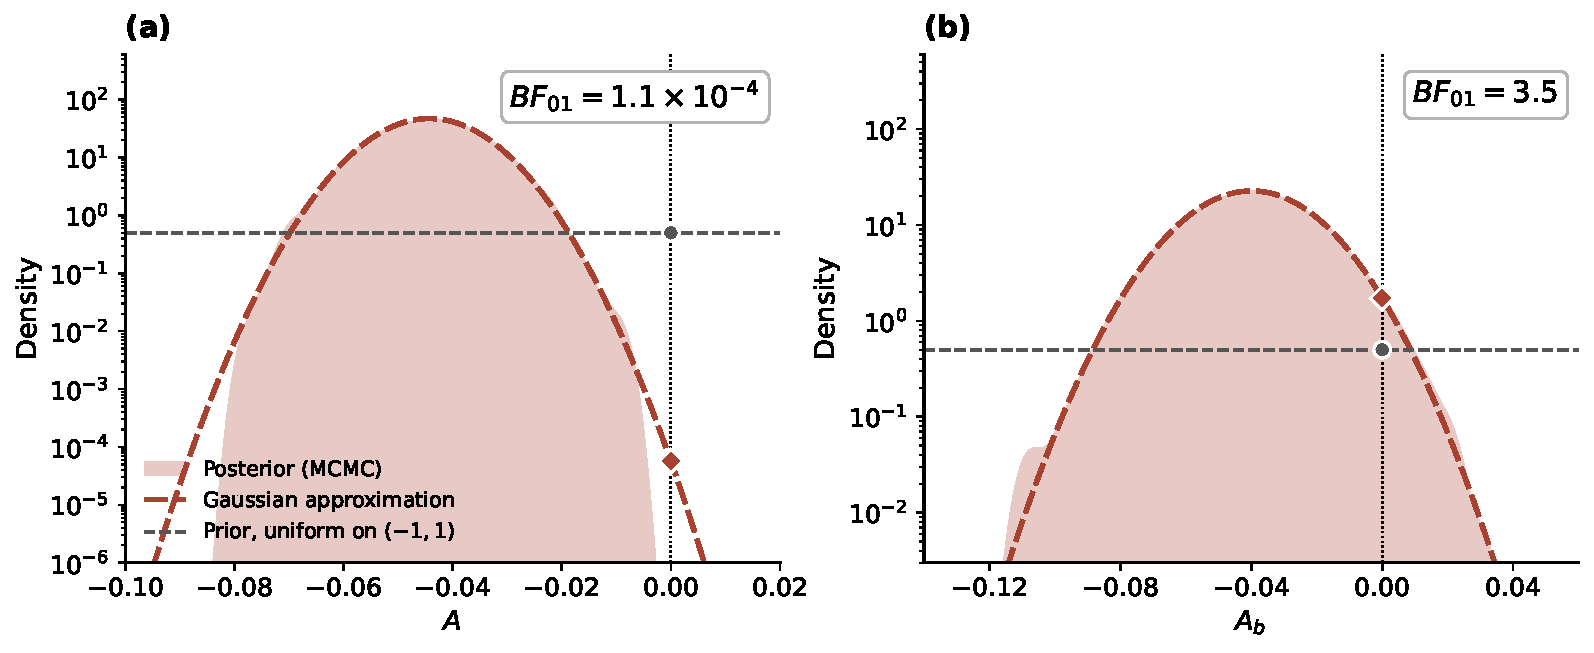
\includegraphics[width=0.95\textwidth]{figures/short_savage_dickey.pdf}
\caption{Savage-Dickey ratio for (a) $A$ and (b) $A_b$: marginal posterior (histogram of the chain and Gaussian approximation) and prior density, logarithmic scale. The Bayes factor $BF_{01}$ is the ratio of the two densities at zero (dots). For $A$ the posterior density at zero is $10^{-4}$ times the prior one; for $A_b$, $2.3$ standard deviations from zero, it is higher than the prior density, and the data favor $A_b=0$.}
\label{fig:bayes_sd}
\end{figure*}

The same test on the background asymmetry shows the Ockham factor at work: $A_b=-0.040\pm0.018$ is $2.3$ standard deviations from zero, yet $BF_{01}(A_b=0)\approx3.5$, because the likelihood gain does not compensate for spreading the prior over $(-1,1)$; unlike for $A$, the preference changes sign with the prior width (Fig.~\ref{fig:checks_bf}, crossing at $W\approx0.3$). Of the Bayesian results only the Bayes factor depends on the prior; the interval of $A$ does not (Sec.~\ref{sec:bayes_posterior}). A negative $A_b$ is plausible given the misidentified $B^\pm\to K^\pm\pi^+\pi^-$ and $\pi^\pm K^+K^-$ decays; $A_b$ is kept free in the nominal model and fixing it to zero is one of the systematic variants (Sec.~\ref{sec:syst}).
 \emph{Model Adequacy: Goodness of Fit and Posterior Predictive Check}: the model does not reach $\chi^2/\mathrm{ndof}\approx1$ ($164.1/88$), mainly because the signal tails are heavier than a Gaussian, but $\Araw$ changes by only $-0.0002$ with a Crystal Ball signal.
\subsection{Metropolis-Hastings and the Ensemble Sampler}
\label{app:theory}
\emph{In short: Metropolis-Hastings accepts a proposal with a ratio that satisfies detailed balance; the affine-invariant ensemble move samples correlated posteriors without tuning, and $N/\tau$ is the effective length of a chain.}
The Metropolis-Hastings algorithm builds a Markov chain whose stationary distribution is the target $\pi(\theta)$: from the state $x$ a point $y$ is proposed from $q(y\mid x)$ and accepted with probability $\min\!\big[1,\pi(y)\,q(x\mid y)/(\pi(x)\,q(y\mid x))\big]$, which satisfies detailed balance. Its efficiency depends on how the proposal is matched to the (here correlated) posterior. The ensemble sampler used for the nominal fit~\cite{goodman_weare,emcee} evolves $K$ walkers; to update the walker $X_k$ it picks another walker $X_j$ and proposes $Y=X_j+Z\,(X_k-X_j)$, with $Z\in[1/a,a]$ drawn from $g(z)\propto z^{-1/2}$ ($a=2$), and accepts it with probability $\min\!\big[1,Z^{d-1}\pi(Y)/\pi(X_k)\big]$ ($d$ the number of parameters). The move is invariant under affine transformations of the parameters, so a strongly correlated, elongated posterior is as easy to sample as a spherical one, and it needs no hand-tuned proposal covariance.
Successive states of a chain are correlated. The integrated autocorrelation time of a parameter is $\tau=1+2\sum_{t\geq1}\rho(t)$, with $\rho(t)$ the autocorrelation of the chain at lag $t$, and a chain of $N$ steps contains $N_{\mathrm{eff}}=N/\tau$ effectively independent samples, so that the Monte Carlo error of a posterior mean is $\sigma/\sqrt{N_{\mathrm{eff}}}$. The estimate of $\tau$ is itself reliable only for $N\gtrsim50\,\tau$~\cite{emcee}.
\subsection{Sampling and Convergence Diagnostics}
\emph{In short: $32$ walkers for $25{,}000$ steps give $N/\tau\geq113$ autocorrelation times for every parameter, and runs started over the whole prior box converge to the same single mode.}
The posterior was sampled with the affine-invariant ensemble sampler of Goodman and Weare~\cite{goodman_weare} as implemented in \texttt{emcee}~\cite{emcee} (the stretch move, the autocorrelation time and the effective sample size are described in Sec.~\ref{app:theory}). The maximum of the posterior was first located numerically (Nelder-Mead), and 32 walkers were initialized in a narrow ball around it and run for $25{,}000$ steps, with the first $4166$ ($1/6$) discarded as burn-in, leaving $6.7\times10^5$ samples; the mean acceptance fraction is $0.38$. Convergence was checked through the integrated autocorrelation time of each parameter, $\tau=1+2\sum_{t\geq1}\rho(t)$, with $\rho(t)$ the autocorrelation of the chain at lag $t$. We find $\tau\in[147,183]$ steps, the longest for the background-shape parameters: the post-burn-in chain is $N/\tau\geq113$ autocorrelation times long for every parameter, above the threshold of $50$ recommended for a reliable estimate of $\tau$~\cite{emcee}, and corresponds to $\gtrsim3600$ effectively independent samples per parameter. To check that the chain is not trapped near its starting point, the fit was repeated twice with the walkers initialized uniformly over the whole prior box and the first half of the chain discarded: both runs converge to the same single mode, with $\Araw=-0.0446$ and $-0.0442$, the same intervals and the same values of all other parameters as the nominal fit. The trace plot of such a run (Fig.~\ref{fig:bayes_trace}) shows all walkers reaching the bulk of the posterior within $\sim$2000 steps, the background fraction $f_+$ last, well inside the discarded half of the chain.

\begin{figure*}[t]
\centering
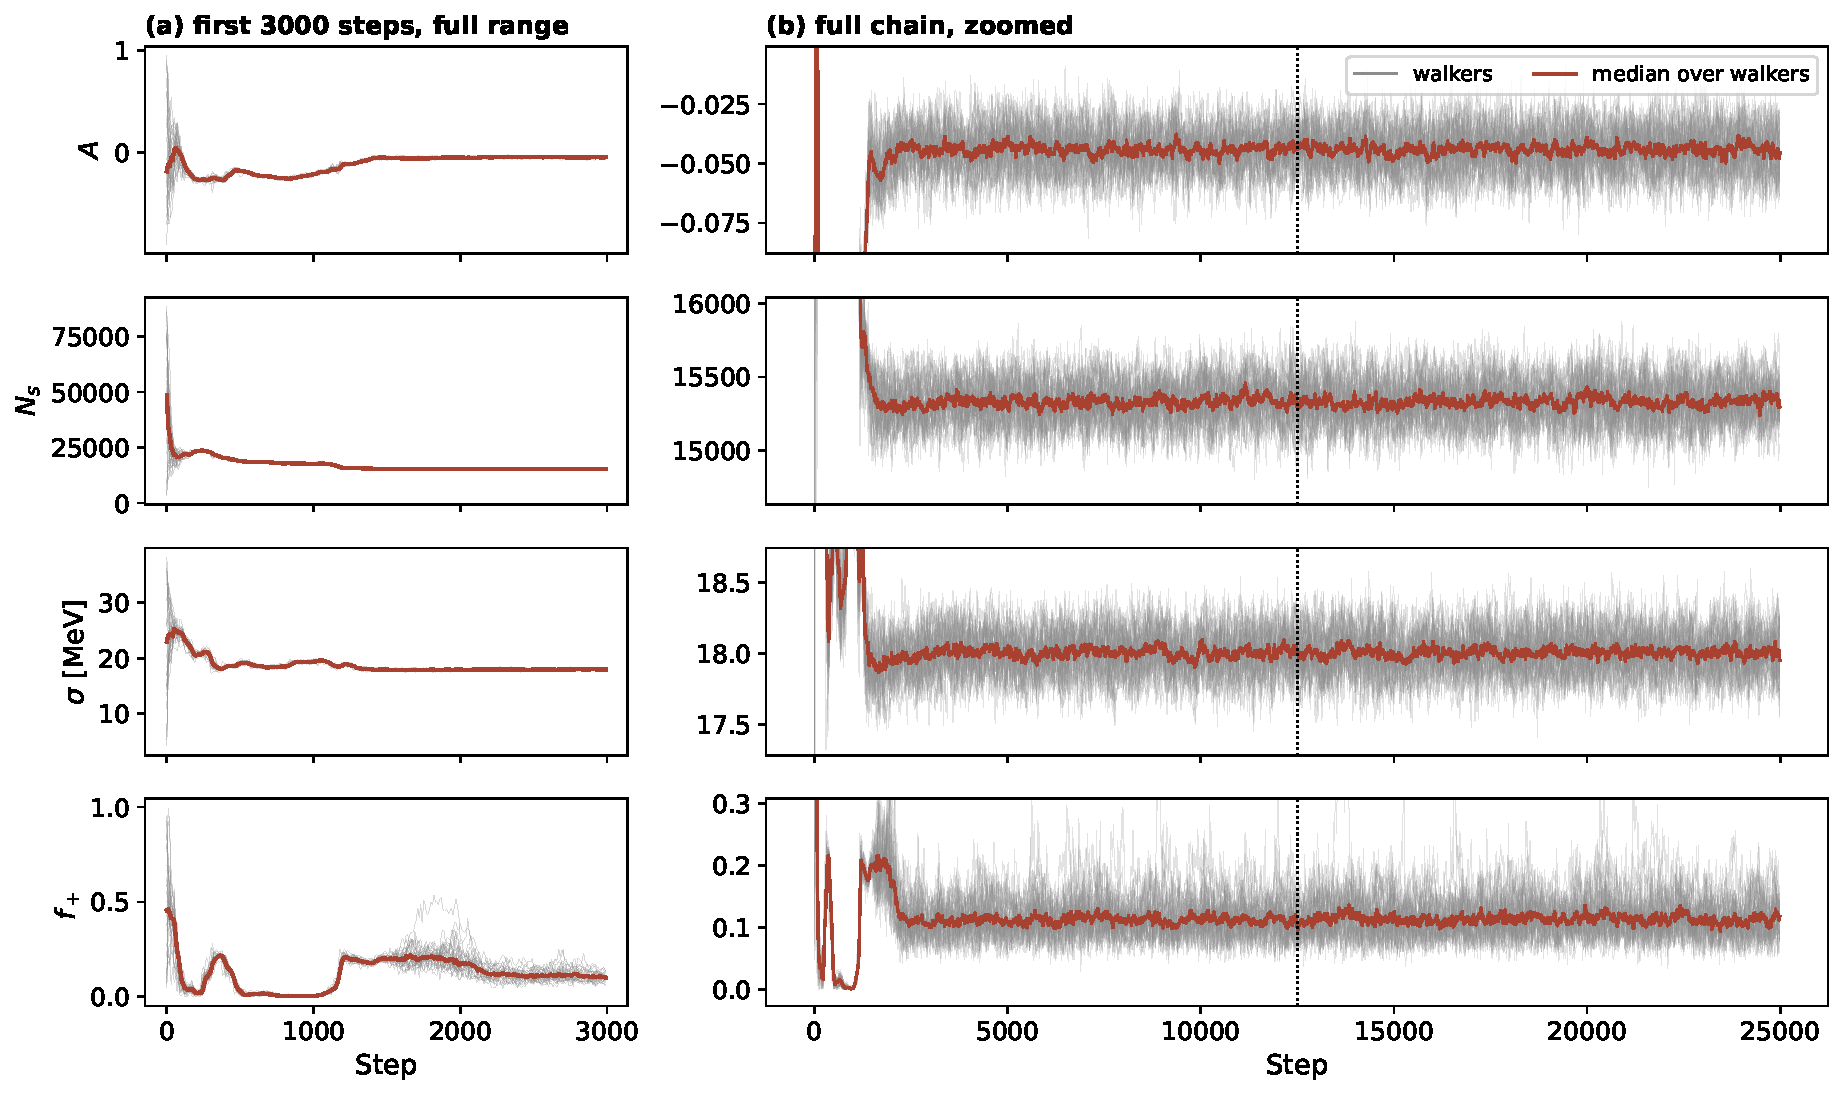
\includegraphics[width=0.95\textwidth]{figures/bayes_nominal_trace.pdf}
\caption{Trace plot of the nominal fit with the 32 walkers initialized uniformly over the prior box (one grey line per walker, every 10th step; colored: median over the walkers), for $A$, $N_s$, $\sigma$ and the steep-background fraction $f_+$. Left: first 3000 steps, full range; right: whole chain, zoomed on the posterior. The first half of the chain (dotted line) is discarded as burn-in.}
\label{fig:bayes_trace}
\end{figure*}

\subsection{Equal-Tailed and Highest-Posterior-Density Intervals}
\label{sec:checks_hpd}
\emph{In short: for $A$ and $A_b$ the two kinds of $68\%$ interval coincide; they differ for the skewed parameters, whose highest-posterior-density interval is shifted towards the mode.}
Table~\ref{tab:checks_hpd} compares the equal-tailed interval (percentiles $15.9\%$--$84.1\%$) with the interval of highest posterior density, the shortest containing $68.3\%$, for the parameters of interest and for three skewed nuisance parameters.

\begin{table}[h]
\centering
\resizebox{\ifdim\width>\linewidth\linewidth\else\width\fi}{!}{\begin{tabular}{lcccc}
\toprule
Parameter & median & equal-tailed & HPD & skewness \\
\midrule
$A$ & $-0.0442$ & $[-0.0529,-0.0358]$ & $[-0.0525,-0.0355]$ & $+0.01$ \\
$A_b$ & $-0.0400$ & $[-0.0575,-0.0224]$ & $[-0.0575,-0.0225]$ & $+0.01$ \\
$f_+$ & $0.114$ & $[0.089,0.145]$ & $[0.084,0.138]$ & $+0.90$ \\
$f_-$ & $0.209$ & $[0.174,0.248]$ & $[0.168,0.241]$ & $+0.33$ \\
$\lambda_1^+$ [MeV$^{-1}$] & $0.0350$ & $[0.0281,0.0431]$ & $[0.0274,0.0423]$ & $+0.52$ \\
\bottomrule
\end{tabular}}
\caption{Equal-tailed and highest-posterior-density $68\%$ intervals and skewness of the marginal posteriors.}
\label{tab:checks_hpd}
\end{table}

\subsection{Posterior Summaries and Model Comparison}
\emph{In short: equal-tailed and HPD intervals, the Jeffreys scale for Bayes factors, the Ockham effect of the prior width and the definition of the posterior predictive $p$-value.}
The credible intervals quoted are the equal-tailed ones (the $16\%$--$84\%$ quantiles for $68\%$); the highest-posterior-density (HPD) interval is the shortest interval with the same probability and coincides with it for a symmetric posterior. A Bayes factor $BF_{ij}=P(D\mid H_i)/P(D\mid H_j)$ is interpreted with the Jeffreys scale~\cite{jeffreys,kass_raftery}: values between $1$ and $3$ are barely worth mentioning, $3$--$10$ substantial, $10$--$30$ strong, $30$--$100$ very strong and above $100$ decisive. The evidence automatically penalizes unnecessary freedom (Ockham's razor): for a Gaussian posterior much narrower than a uniform prior of width $2W$ the Savage-Dickey ratio of $A=0$ is proportional to $W$, so widening the prior of $A$ favors the null hypothesis by construction, which is why the dependence on $W$ is reported.
The posterior predictive check compares the data $y$ with replicas $y^{\mathrm{rep}}$ simulated from the model at parameters drawn from the posterior, through a discrepancy statistic $T$: the posterior predictive $p$-value is $p_B=P\big(T(y^{\mathrm{rep}},\theta)\geq T(y,\theta)\mid y\big)$~\cite{gelman_ppc}. Values close to $0$ or $1$ signal a feature of the data that the model does not reproduce; a statistic that the fit adjusts directly (for example the total asymmetry, when $A$ is a free parameter) is reproduced by construction and tests nothing.
\subsection{Savage--Dickey Densities of the Parameters}
\label{app:sd_densities}
\emph{In short: the posterior and prior densities at the null value, which give the Bayes factors of the main text.}

\subsection{Priors and Bayes Factors}
\label{sec:checks_prior}
\emph{In short: no change of the prior on the nuisance parameters or of its parametrization moves $A$ by more than $0.0002$; the Bayes factor of $A=0$ scales with the prior width, and the evidence computed by direct integration agrees in order of magnitude with the Savage-Dickey ratio.}
The posterior was reweighted, without new sampling, to other priors: logarithmically uniform yields and slopes, a prior uniform in the lifetimes $1/\lambda$, and a prior flat in $(N_s^+,N_s^-)$ and $(N_b^+,N_b^-)$ instead of $(N_s,A)$ and $(N_b,A_b)$, which differ by the Jacobian $N_s/2$ (Table~\ref{tab:checks_prior}). The largest shift is $0.0002$, and the effective sample size of the reweighted chain is stated.

\begin{table}[h]
\centering
\resizebox{\ifdim\width>\linewidth\linewidth\else\width\fi}{!}{\begin{tabular}{lccc}
\toprule
Prior & $A$ (median) & $68\%$ interval & ESS \\
\midrule
Nominal (uniform) & $-0.0442$ & $[-0.0529,-0.0358]$ & $20000$ \\
Log-uniform $N_s$, $N_b$ & $-0.0442$ & $[-0.0529,-0.0358]$ & $19993$ \\
Log-uniform slopes & $-0.0440$ & $[-0.0528,-0.0356]$ & $12306$ \\
Uniform in $1/\lambda$ & $-0.0444$ & $[-0.0526,-0.0360]$ & $153$ \\
Flat in $(N_s^+,N_s^-)$ & $-0.0442$ & $[-0.0529,-0.0358]$ & $19999$ \\
Flat in $(N_s^\pm)$ and $(N_b^\pm)$ & $-0.0442$ & $[-0.0529,-0.0358]$ & $19993$ \\
\bottomrule
\end{tabular}}
\caption{Posterior of $A$ under alternative priors, by importance reweighting of the chain; ESS: effective sample size of the $20{,}000$ thinned samples.}
\label{tab:checks_prior}
\end{table}

The Bayes factor $BF_{01}=p(A=0\mid D)/\pi(0)$ is proportional to the density of the prior at zero, $\pi(0)=1/(2W)$ for a uniform prior on $(-W,W)$ (Fig.~\ref{fig:checks_bf}): for $A$ it stays below $10^{-2}$ for every width up to $W=1$ (decisive evidence for $A\neq0$ whatever the prior), while for $A_b$ it crosses $1$ at $W\simeq0.3$, which is the content of the Lindley paradox. The same evidence was computed by direct numerical integration over $A$ on a grid, $Z_1=\int L\,\pi\,dA$ with the nuisance parameters fixed at the maximum of the posterior, the method that is not feasible for twelve parameters: it gives $K_{01}=7.0e-05$, against $1.3e-04$ with the profile likelihood and $1.1e-04$ for the Savage-Dickey ratio, which marginalizes the nuisance parameters; the three values are of the same order and the conclusion is the same.
The Savage-Dickey ratio also tests the equality of the background shapes of the two charges, one parameter at a time, with the difference $\delta=\theta^+-\theta^-$: $BF_{01}=3.1$ for the steep slope $\lambda_1$ (difference at $0.8\sigma$), $2.2$ for $\lambda_2$ ($2.4\sigma$) and $1.1$ for the fraction $f$ ($2.0\sigma$). The data are not able to distinguish the shapes, with a weak preference for equal ones: this is why the variant with a shared shape moves $A$ by $-0.0037$ and is part of the systematic uncertainty, without being preferred.
\subsection{Model Adequacy: Goodness of Fit and Posterior Predictive Check}
\label{sec:bayes_gof}
\emph{In short: the model does not reach $\chi^2/\mathrm{ndof}\approx1$ ($164.1/88$), mainly because the signal tails are heavier than a Gaussian, but $\Araw$ changes by only $-0.0002$ with a Crystal Ball signal.}

A binned comparison of data and posterior-median model ($\chi^2=\sum(\text{obs}-\text{exp})^2/\text{exp}$ over 50 bins of $10\,\MeV$ per charge, $100-12=88$ degrees of freedom) gives $\chi^2=164.1/88$ ($p=1.6\times10^{-6}$), with $95.4$ for $B^+$ and $68.7$ for $B^-$. The largest pulls, in the $B^+$ sample, sit on the two flanks of the peak, about $\pm3\sigma$ from $\mu$ (Fig.~\ref{fig:bayes_fit}): the observed signal shape has heavier tails than a Gaussian. Replacing the Gaussian by a Crystal Ball shape~\cite{skwarnicki}, a Gaussian core with a power-law low-mass tail,
\begin{equation}
S_{\mathrm{CB}}(x)\propto
\begin{cases}
e^{-x^2/2}, & x>-\beta,\\[2pt]
\left(\frac{\kappa}{\beta}\right)^{\kappa} e^{-\beta^2/2}\left(\frac{\kappa}{\beta}-\beta-x\right)^{-\kappa}, & x\leq-\beta,
\end{cases}
\label{eq:cb}
\end{equation}
with $x=(m-\mu)/\sigma$, $\beta$ the point where the tail starts (in units of $\sigma$) and $\kappa$ its power, both free, improves the fit to $\chi^2=131.0/86$ ($p=1.3\times10^{-3}$, $\beta=1.71$, $\kappa=35$) but moves $\Araw$ by only $-0.0002$ (Table~\ref{tab:gof}). The asymmetry does not depend on the signal shape even though none of the models reaches $\chi^2/\text{ndof}\approx1$. The Gaussian is nevertheless kept as the nominal signal model, common to the two analyses: the Crystal Ball adds two tail parameters that are poorly constrained (its power $\kappa$ runs to large values), and the effect of the signal shape on $\Araw$ is covered by the systematic study (Sec.~\ref{sec:syst}).

\begin{table}[!t]
\centering
\begin{tabular}{lccc}
\toprule
Model & $\Araw$ & $\chi^2$/ndof & $p$ \\
\midrule
Nominal & $-0.0443$ & $164.1/88$ & $2\times10^{-6}$ \\
Crystal Ball signal & $-0.0445$ & $131.0/86$ & $1\times10^{-3}$ \\
$\mu$, $\sigma$ per charge & $-0.0443$ & $164.2/86$ & $8\times10^{-7}$ \\
Shared bkg.\ shape & $-0.0480$ & $174.1/91$ & $4\times10^{-7}$ \\
Symmetric bkg.\ ($A_b=0$) & $-0.0471$ & $169.8/89$ & $5\times10^{-7}$ \\
Single exponential & $-0.0480$ & $297.7/92$ & $2\times10^{-23}$ \\
\bottomrule
\end{tabular}
\caption{$\Araw$ (posterior median) and goodness of fit of the nominal model (Gaussian signal, double exponential per charge) and of the alternative signal and background models, same data and window.}
\label{tab:gof}
\end{table}

The background model is constrained by the data much more strongly. A single exponential per charge is rejected ($\chi^2=297.7/92$, $\Delta\chi^2=134$ for four fewer parameters), and so it is not used even as a systematic variant (Sec.~\ref{sec:syst}). A shape shared between the two charges ($\Delta\chi^2=10.0$ for three fewer parameters) and a charge-symmetric background ($\Delta\chi^2=5.7$ for one fewer) are acceptable descriptions and shift $\Araw$ by $-0.0037$ and $-0.0028$: the background treatment is the largest model dependence of the fit. The lower edge of the window is a compromise between two failures. Extending the window to $5050\,\MeV$ degrades the fit ($\chi^2=217.4/98$), because the double exponential no longer follows the background further below the peak; raising it to $5150\,\MeV$ removes most of the region that constrains the steep component, which becomes poorly identified -- the chain for its fraction $f_+$ mixes slowly ($N/\tau=10$) -- while $\Araw$ itself is unchanged ($-0.0444$).

The binned $\chi^2$ uses the posterior medians only. A posterior predictive check~\cite{gelman_ppc} accounts for the posterior uncertainty and tests specific features of the data: for $1000$ parameter sets $\theta_j$ drawn from the posterior, a dataset $y^{\mathrm{rep}}_j$ is generated from the model, and a discrepancy $T(y,\theta_j)$ is computed both on the replica and on the data; the posterior predictive $p$-value is $p_B=P\big(T(y^{\mathrm{rep}},\theta)\geq T(y,\theta)\mid y\big)$. For the binned $\chi^2$ the replicas give $104\pm15$ and the data $175$ (median over $\theta_j$): none of the replicas reaches the observed value ($p_B<10^{-3}$), with the misfit concentrated in the $B^+$ sample ($p_B<10^{-3}$, against $0.03$ for $B^-$). The counting asymmetries of the whole window ($p_B=0.996$) and of the signal window ($0.99$) are reproduced, but this is expected and not informative: $A$ is a free parameter, so the replicas are centred on the observed value by construction. The asymmetry of the sidebands ($0.73$), which the fit constrains less directly, is also reproduced (Fig.~\ref{fig:bayes_ppc}). The check therefore shows that the model misdescribes the shape of the spectrum, mainly the signal tails, and does not reveal a charge-dependent distortion of the sidebands; that $\Araw$ does not depend on the signal shape is shown directly by its stability under the Crystal Ball model (Table~\ref{tab:gof}).

\begin{figure*}[t]
\centering
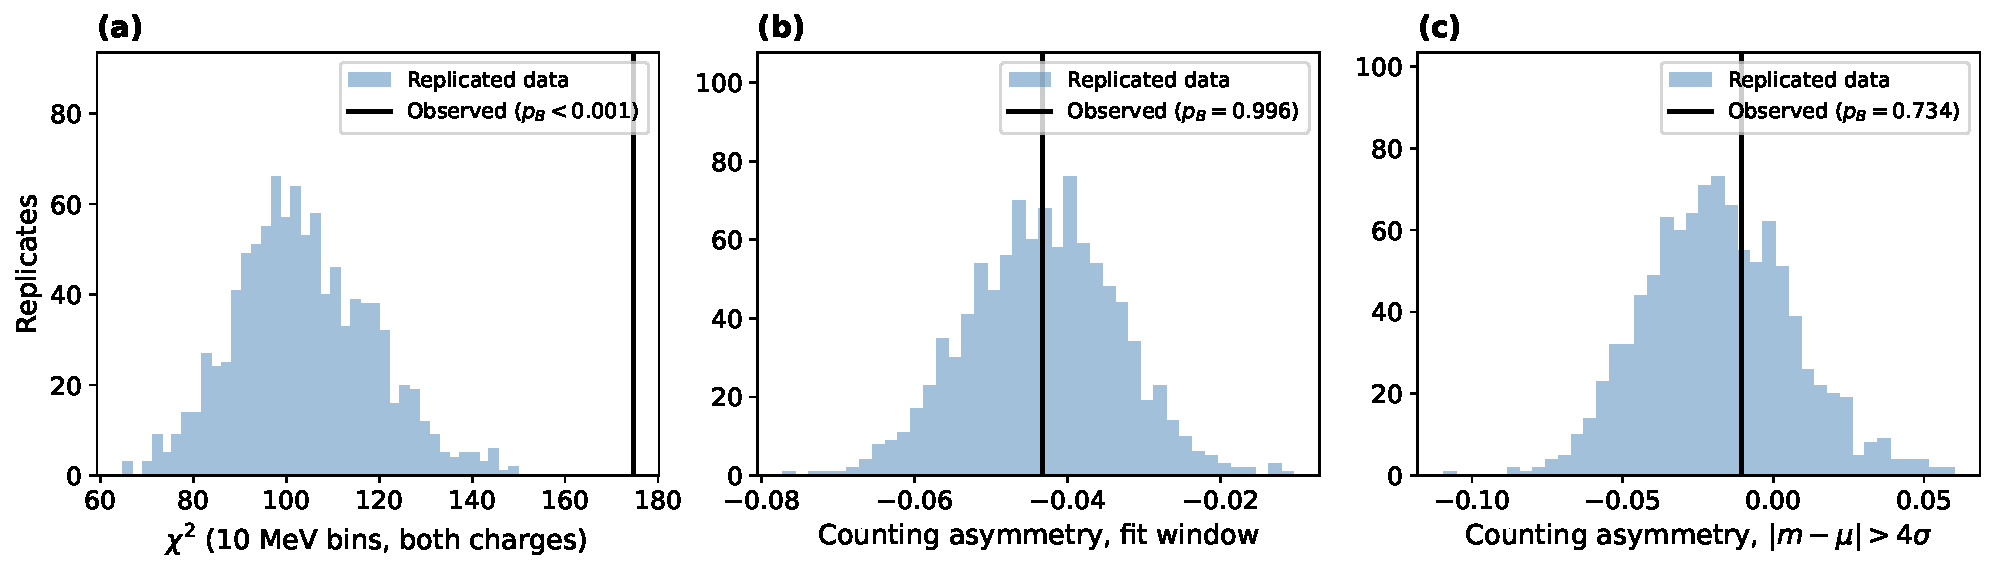
\includegraphics[width=0.95\textwidth]{figures/bayes_nominal_ppc.pdf}
\caption{Posterior predictive check: distributions of three discrepancies over $1000$ datasets replicated from posterior draws, compared with the observed values. (a) binned $\chi^2$; (b) and (c) counting asymmetry of the fit window and of the sidebands.}
\label{fig:bayes_ppc}
\end{figure*}

\subsection{Posterior Predictive Check with Statistics Not Fitted by the Model}
\label{sec:checks_ppc}
\emph{In short: the asymmetry in slices of the mass, which the model predicts, is reproduced ($p_B=0.67$), and the difference between the $\chi^2$ of the two charges is at the edge of the replicas ($p_B=0.08$).}
Section~\ref{sec:bayes_gof} noted that the counting asymmetries of the window are fitted by construction. Two statistics that are not adjusted directly were therefore used (Fig.~\ref{fig:checks_ppc}): the asymmetry in ten slices of $50\,\MeV$ of the mass against the one predicted by the model from the same posterior draw, which tests that the charge asymmetry follows the mixture of signal and background, $T=\sum_s(A_s-\bar A_s)^2/\sigma_s^2$, and the difference $\chi^2(B^+)-\chi^2(B^-)$ of the binned fit. The slice asymmetries are reproduced; the difference of the $\chi^2$ is $27$ in the data against $-0\pm15$ in the replicas, a $1.8\sigma$ excess that restates that the misfit is concentrated in the $B^+$ sample.

\begin{figure*}[t]
\centering
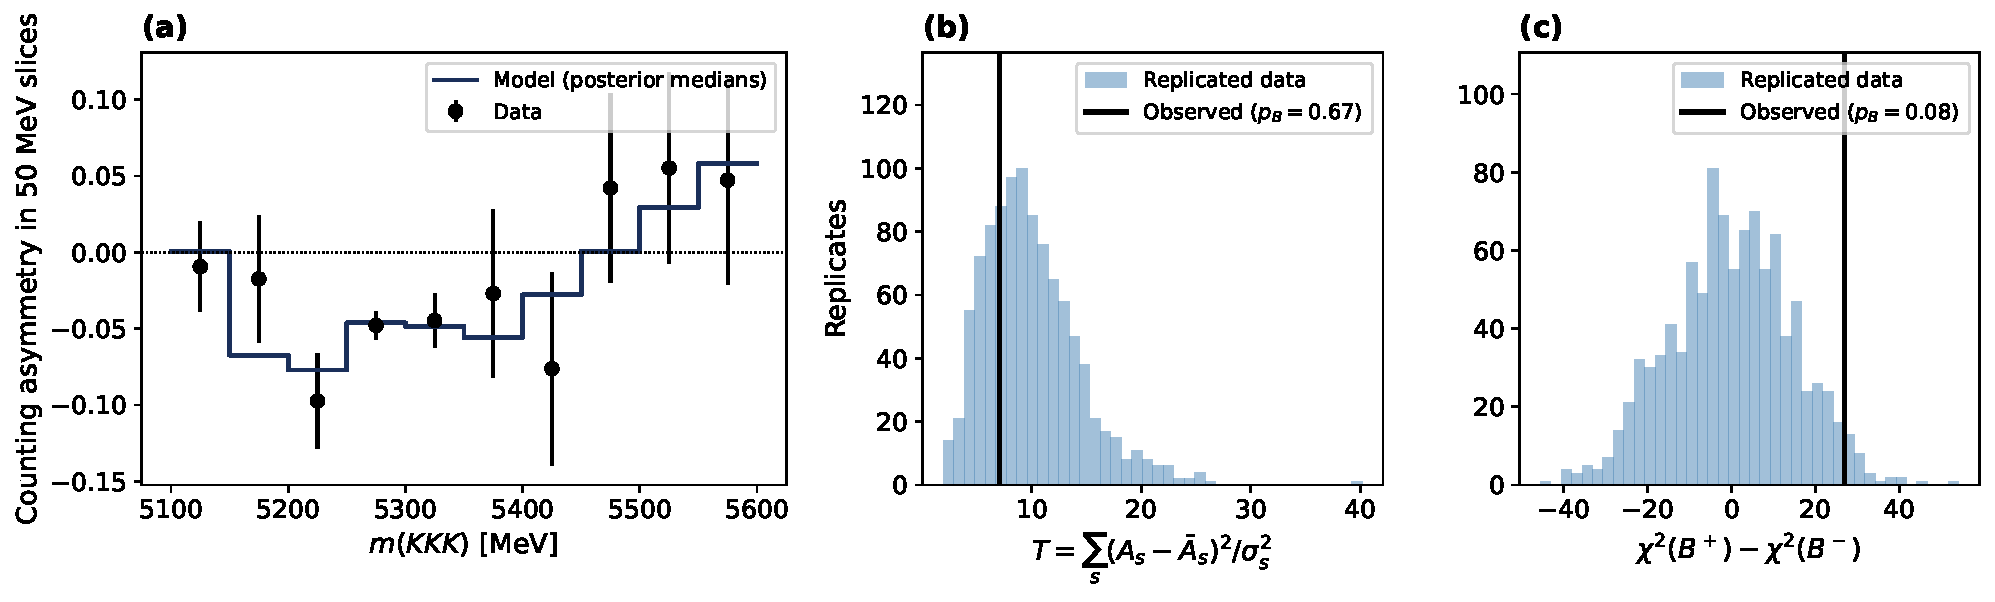
\includegraphics[width=0.95\textwidth]{figures/validation_ppc_unfitted.pdf}
\caption{(a) Counting asymmetry in slices of $50\,\MeV$ of the mass, data and model. (b) Distribution of $T=\sum_s(A_s-\bar A_s)^2/\sigma_s^2$ over $1000$ replicas and observed value. (c) The same for $\chi^2(B^+)-\chi^2(B^-)$.}
\label{fig:checks_ppc}
\end{figure*}

\subsection{Robustness Checks: Polarity, Prior and Charm Vetoes}
\label{sec:bayes_checks}
\emph{In short: $\Araw$ agrees between the two magnet polarities ($0.7\sigma$) and does not depend on the prior; the $D^0$ veto moves it by $2.3$ times the expected statistical spread.}

The fit was repeated separately on the two magnet polarities, whose left-right detection asymmetries are opposite and partially cancel in the combined sample: $\Araw(\text{down})=-0.0497\pm0.0112$ ($n=11{,}636$) and $\Araw(\text{up})=-0.0378\pm0.0129$ ($n=8095$); the Frequentist fits give $-0.0492\pm0.0111$ and $-0.0374\pm0.0131$, and the sum of their profile likelihoods $-0.0443\pm0.0084$ (Sec.~\ref{sec:checks_profile}). They differ by $0.7\sigma$, so there is no indication that the asymmetry is an artifact of one polarity (Fig.~\ref{fig:bayes_magnet}). A narrower prior, $A\in(-0.3,0.3)$, leaves the posterior unchanged ($\Araw=-0.0443$), as expected for a posterior far from the prior bounds; the prior width matters only for the Bayes factor (Sec.~\ref{sec:bayes_factor}).

\begin{figure}[h]
\centering
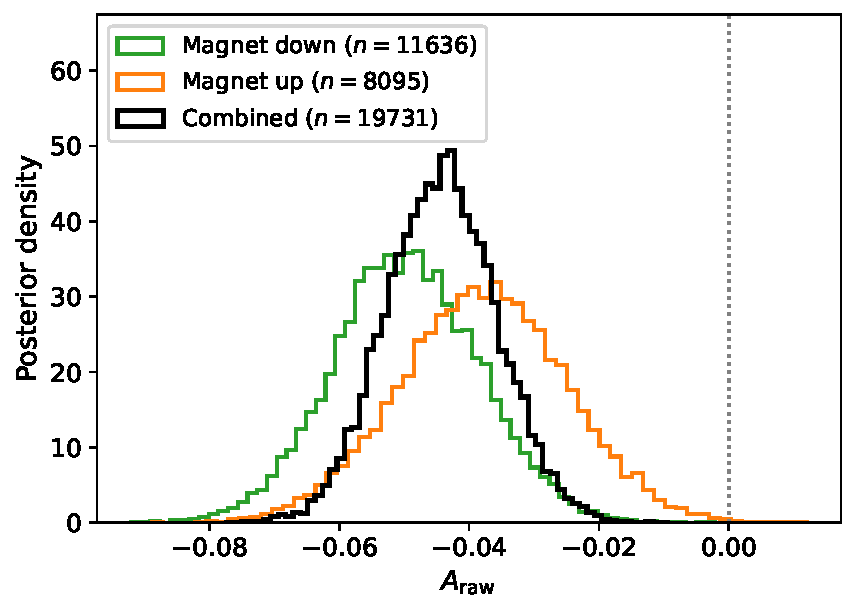
\includegraphics[width=\columnwidth]{figures/bayes_nominal_magnet.pdf}
\caption{Posterior of $\Araw$ for the magnet-down, magnet-up and combined samples.}
\label{fig:bayes_magnet}
\end{figure}

The sample contains $B^\pm$ decays through intermediate charm states, $B^\pm\to D^0K^\pm$, $J/\psi K^\pm$ and $\chi_{c0}K^\pm$ with $D^0$, $J/\psi$, $\chi_{c0}\to K^+K^-$, which are visible as peaks in the opposite-sign $m(K^+K^-)$ spectra. They are part of the $B^\pm\to K^\pm K^+K^-$ final state and are kept in the nominal sample; removing them changes the observable, from the asymmetry of all $B^\pm\to K^\pm K^+K^-$ decays to that of the charmless ones, so the vetoes are reported as an informative check rather than as a systematic variation. A candidate is vetoed if either opposite-sign pair, $m(H1,H2)$ or $m(H1,H3)$, lies within $\pm30\,\MeV$ of the $D^0$ or $J/\psi$ mass or within $\pm60\,\MeV$ of the $\chi_{c0}$ mass (world-average masses; the wider window for the $\chi_{c0}$ reflects its natural width). The $D^0$ veto alone keeps $18{,}744$ candidates and gives $\Araw=-0.0496\pm0.0088$; the three vetoes together keep $16{,}367$ and give $-0.0423\pm0.0094$. The shifts with respect to the nominal fit, $-0.0053$ and $+0.0020$, compare with expected statistical fluctuations of $0.0023$ and $0.0040$ for a subsample of the nominal one (Sec.~\ref{sec:syst}); the $D^0$ veto moves $\Araw$ by $2.3$ times this amount, i.e.\ the vetoed $D^0K^\pm$ candidates have a less negative asymmetry than the rest of the sample. The analysis was also carried out with a minimal six-parameter model, with a narrower window and a single exponential background, before the nominal model was fixed; it gives a compatible result (Sec.~\ref{sec:bayes_minimal}).
\subsection{Toy-MC Coverage Validation}
\label{sec:bayes_toymc}
\emph{In short: $200$ toy-MC experiments give coverage $0.65\pm0.03$ ($68\%$) and $0.93\pm0.02$ ($95\%$), consistent with nominal, with unbiased estimates and pulls of width $1.04$.}

A credible interval is a probability statement on $A$ given the data and the prior, whereas the nominal coverage of a confidence interval is a property of the procedure (Sec.~\ref{sec:frequentist}). With flat priors and $\sim2\times10^4$ events the two intervals coincide numerically (Sec.~\ref{sec:bayes_posterior}), but nothing guarantees the coverage of the credible interval, so it was checked: 200 toy-MC datasets were generated from the fitted model (parametric bootstrap, with the posterior medians as ground truth and Poisson-fluctuated yields for each charge and component; the truncated Gaussian and exponential masses are drawn with the transformation method, i.e.\ by inverting their cumulative distributions) and each was refit with the nominal procedure and a $12{,}000$-step chain. The fraction of replicas whose interval contains the injected $A$ is $0.650\pm0.033$ for the 68\% CI and $0.930\pm0.015$ for the 95\% CI (binomial uncertainties), $1.0\sigma$ and $1.3\sigma$ below nominal: the coverage is consistent with nominal. The estimates themselves are unbiased and their spread matches the reported uncertainty (Fig.~\ref{fig:bayes_toys}): their mean differs from the injected value by $-0.0002\pm0.0006$, their standard deviation, $0.0088$, agrees with the posterior standard deviation of the data fit, $0.0085$, and the pulls have mean $-0.03\pm0.07$ and standard deviation $1.04$.

\begin{figure}[h]
\centering
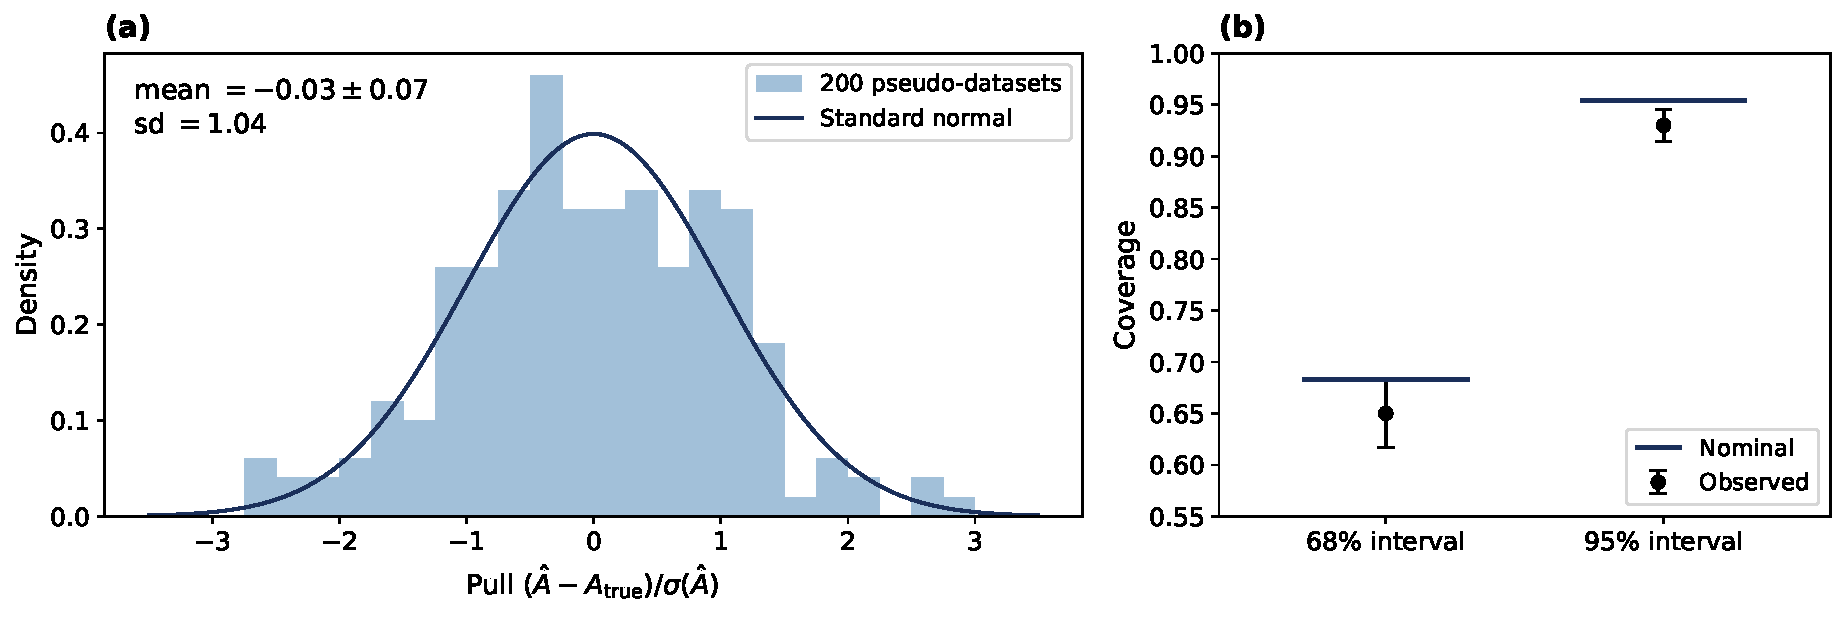
\includegraphics[width=\columnwidth]{figures/bayes_nominal_toys.pdf}
\caption{Toy-MC validation, 200 toy-MC datasets. (a) Pulls $(\hat A-A_{\mathrm{true}})/\sigma(\hat A)$, with $\hat A$ and $\sigma(\hat A)$ the posterior median and standard deviation of each replica, compared with a standard normal. (b) Fraction of replicas whose 68\% and 95\% credible intervals contain the injected value, with binomial uncertainties, and the nominal coverage.}
\label{fig:bayes_toys}
\end{figure}

The toy chains are shorter than the nominal one, and in 124 of the 200 replicas the slowest-mixing parameter, always a background-shape parameter, has $N/\tau<50$ (median $48$, minimum $22$). The criterion on the slowest parameter is conservative for the quantity tested here: for $A$ itself the median autocorrelation time is $156$ steps, so each chain is at least $45$ autocorrelation times long in $A$ and provides $\gtrsim1400$ effectively independent samples of it. The Monte Carlo error on the percentiles of $A$ is then a few per cent of $\sigma(A)$, negligible against the binomial uncertainty of the coverage, and the replicas with $N/\tau<50$ do not show a lower coverage than the others ($0.69$ for the $68\%$ interval, against $0.58\pm0.06$ for the $76$ replicas with $N/\tau\geq50$, whose coverage is $1.9$ standard deviations below nominal: the split was made after the fact and $200$ replicas cannot tell a trend from a fluctuation, and the check on the data of Sec.~\ref{sec:freq_coverage} gives the nominal coverage). This is a closure test of the inference procedure: since the toys are generated from the same model that is fitted, it does not probe the model mismatch of Sec.~\ref{sec:bayes_gof}, which is instead addressed by the systematic study.
\subsection{Metropolis-Hastings Sampler and Published Likelihood}
\label{sec:checks_mh}
\emph{In short: an own Metropolis-Hastings sampler reproduces the posterior of the ensemble sampler, and the profile likelihood is given in a table, so that the result can be combined with others.}
The algorithm of the ensemble sampler was replaced by the basic Metropolis-Hastings one: a Gaussian proposal with the covariance of the posterior scaled by $2.38^2/d$, $120{,}000$ steps with the first $1/6$ discarded. The acceptance is $0.24$, the integrated autocorrelation time of $A$ is $36$ steps ($2813$ effective samples), and $A=-0.0443$ with $68\%$ interval $[-0.0526,-0.0357]$, against $-0.0443$ and $[-0.0528,-0.0358]$ from the ensemble sampler: the two samplers give the same posterior.
The profile likelihood of $A$ is given in Table~\ref{tab:checks_qa}, together with the Minos intervals, so that other measurements of the same quantity can be combined with this one by adding $q(A)$.

\begin{table}[h]
\centering
\resizebox{\ifdim\width>\linewidth\linewidth\else\width\fi}{!}{\begin{tabular}{r|ccccccccc}
\toprule
$A$ & $-0.08$ & $-0.07$ & $-0.06$ & $-0.05$ & $-0.04$ & $-0.03$ & $-0.02$ & $-0.01$ & $+0.00$ \\
$q(A)$ & $17.9$ & $9.3$ & $3.5$ & $0.5$ & $0.2$ & $2.8$ & $8.1$ & $16.1$ & $27.0$ \\
\bottomrule
\end{tabular}}
\caption{Profile likelihood ratio $q(A)=-2\Delta\ln L$ of the nominal fit (other parameters profiled); minimum at $-0.0441$, Minos intervals $[-0.0526,-0.0356]$ ($68\%$) and $[-0.0607,-0.0275]$ ($95\%$).}
\label{tab:checks_qa}
\end{table}

\FloatBarrier

\section{Systematic Uncertainties and Result}
\label{sec:syst}
\label{app:syst}
\emph{In short: thirteen variants in four groups give a systematic uncertainty of $0.0070$ (Bayesian) and $0.0072$ (Frequentist), dominated by the particle-identification requirement; the final result is $\Araw=-0.0443\pm0.0085\,(\text{stat})\pm0.0070\,(\text{syst})$.}
The systematic study asks how much the result depends on choices of the analysis that the data do not fix. The Frequentist and Bayesian fits share one study, so that the two uncertainties are comparable: the same thirteen variants of the nominal choices, fitted by both methods on exactly the same candidates, and the same rule to combine them. The variants (listed in Table~\ref{tab:syst}) change one choice at a time and fall in four groups: the \emph{window}, the \emph{background} model, the \emph{signal} model and the \emph{preselection} cuts.

\begin{table*}[t]
\centering
\resizebox{\ifdim\width>\linewidth\linewidth\else\width\fi}{!}{\begin{tabular}{llrrrrr}
\toprule
Group & Variant & $n$ & $\Delta$ Bayes & $\sigma_B$ Bayes & $\Delta$ freq. & $\sigma_B$ freq. \\
\midrule
Window & $[5050,5600]$ & $21164$ & $-0.0003$ & $0.0009$ & $-0.0004$ & $0.0005$ \\
 & $[5150,5600]$ & $18566$ & $-0.0001$ & $0.0007$ & $-0.0005$ & $0.0021$ \\
 & $[5100,5450]$ & $19004$ & $+0.0002$ & $0.0009$ & $-0.0001$ & $0.0003$ \\
 & $[5100,5700]$ & $20191$ & $\mathbf{-0.0014}$ & $0.0010$ & $\mathbf{-0.0014}$ & $0.0001$ \\
Background & single exponential (rejected) & $19731$ & $-0.0037$ & -- & $-0.0039$ & -- \\
 & shape shared between charges & $19731$ & $\mathbf{-0.0037}$ & -- & $\mathbf{-0.0040}$ & -- \\
 & symmetric, $A_b=0$ & $19731$ & $-0.0028$ & -- & $-0.0031$ & -- \\
Signal & Crystal Ball & $19731$ & $\mathbf{-0.0002}$ & -- & $\mathbf{-0.0006}$ & -- \\
 & $\mu,\sigma$ per charge & $19731$ & $-0.0000$ & -- & $-0.0001$ & -- \\
Preselection & $\texttt{ProbK}>0.4$ & $26553$ & $-0.0032$ & $0.0038$ & $-0.0032$ & $0.0037$ \\
 & $\texttt{ProbK}>0.6$ & $13981$ & $\mathbf{+0.0058}$ & $0.0048$ & $\mathbf{+0.0058}$ & $0.0050$ \\
 & $\texttt{ProbPi}<0.4$ & $17984$ & $+0.0022$ & $0.0022$ & $+0.0020$ & $0.0023$ \\
 & $\texttt{ProbPi}<0.6$ & $20953$ & $-0.0004$ & $0.0020$ & $-0.0006$ & $0.0017$ \\
\midrule
\multicolumn{3}{l}{Group uncertainties: window / background / signal / preselection} & \multicolumn{2}{c}{$0.0014/0.0037/0.0002/0.0058$} & \multicolumn{2}{c}{$0.0014/0.0040/0.0006/0.0058$} \\
\multicolumn{3}{l}{Total (quadrature)} & \multicolumn{2}{c}{$0.0070$} & \multicolumn{2}{c}{$0.0072$} \\
\bottomrule
\end{tabular}}
\caption{Systematic study common to the Bayesian and Frequentist fits: shift of $\Araw$ for each variant and, for the variants that change the sample, the expected statistical spread $\sigma_B$ of the shift. The largest contributing shift of each group is in bold. The single exponential is rejected by the data and excluded. For the window $[5150,5600]$ the Frequentist uncertainty is scaled from the number of events, since the Hesse matrix of that fit is not accurate.}
\label{tab:syst}
\end{table*}

The shift $\Delta=\Araw^{\mathrm{var}}-\Araw^{\mathrm{nom}}$ of a variant is not necessarily a systematic effect: when a variant changes the sample (window, preselection) the two samples are nested and part of $\Delta$ is a statistical fluctuation of expected size $\sigma_B=\sqrt{|\sigma_{\mathrm{var}}^2-\sigma_{\mathrm{nom}}^2|}$~\cite{barlow}, and such a variant contributes only if $|\Delta|>\sigma_B$. A variant that the data reject ($\Delta\chi^2>25$ on the same data) is excluded: this removes the single exponential ($\Delta\chi^2=134$, Sec.~\ref{sec:bayes_gof}). The largest remaining $|\Delta|$ of each group is its uncertainty, since the variants of a group are alternative descriptions of the same choice, and the groups, being independent choices, are added in quadrature.

The results are in Table~\ref{tab:syst}, and all the Bayesian fits in Table~\ref{tab:bayes_all}. The two methods give the same shifts to within $\sim$$0.0005$ and the same group uncertainties, with totals of $0.0070$ (Bayesian) and $0.0072$ (Frequentist):
\begin{gather*}
\text{Bayesian:}\\ \Araw=-0.0443\pm0.0085\,(\text{stat})\pm0.0070\,(\text{syst}),\\[2pt]
\text{Frequentist:}\\ \Araw=-0.0441\pm0.0085\,(\text{stat})\pm0.0072\,(\text{syst}).
\end{gather*}

\begin{table*}[t]
\centering
\begin{tabular}{lrccc|c}
\toprule
Fit & $n$ & $\Araw$ Bayesian (median) & 68\% CI & $\chi^2$/ndof & $\Araw$ Frequentist \\
\midrule
Nominal & $19731$ & $-0.0443$ & $[-0.0528,-0.0358]$ & $164.1/88$ & $-0.0441\pm0.0085$ \\
\multicolumn{6}{l}{\emph{Systematic variants (Sec.~\ref{sec:syst})}} \\
Window $[5050,5600]$ & $21164$ & $-0.0446$ & $[-0.0531,-0.0362]$ & $217.4/98$ & $-0.0445\pm0.0085$ \\
Window $[5150,5600]$ & $18566$ & $-0.0444$ & $[-0.0528,-0.0359]$ & $141.5/78$ & $-0.0446\pm0.0088$$^\dagger$ \\
Window $[5100,5450]$ & $19004$ & $-0.0440$ & $[-0.0524,-0.0357]$ & $136.9/58$ & $-0.0442\pm0.0085$ \\
Window $[5100,5700]$ & $20191$ & $-0.0456$ & $[-0.0540,-0.0373]$ & $200.2/108$ & $-0.0455\pm0.0085$ \\
Single exponential & $19731$ & $-0.0480$ & $[-0.0564,-0.0395]$ & $297.7/92$ & $-0.0481\pm0.0085$ \\
Background shape shared & $19731$ & $-0.0480$ & $[-0.0564,-0.0397]$ & $174.1/91$ & $-0.0481\pm0.0083$ \\
Symmetric background & $19731$ & $-0.0471$ & $[-0.0552,-0.0388]$ & $169.8/89$ & $-0.0472\pm0.0084$ \\
Crystal Ball signal & $19731$ & $-0.0445$ & $[-0.0529,-0.0363]$ & $131.0/86$ & $-0.0447\pm0.0085$ \\
$\mu,\sigma$ per charge & $19731$ & $-0.0443$ & $[-0.0527,-0.0356]$ & $164.2/86$ & $-0.0442\pm0.0087$ \\
$\texttt{ProbK}>0.4$ & $26553$ & $-0.0474$ & $[-0.0550,-0.0399]$ & $175.6/88$ & $-0.0473\pm0.0076$ \\
$\texttt{ProbK}>0.6$ & $13981$ & $-0.0385$ & $[-0.0482,-0.0289]$ & $145.0/88$ & $-0.0384\pm0.0099$ \\
$\texttt{ProbPi}<0.4$ & $17984$ & $-0.0421$ & $[-0.0506,-0.0333]$ & $150.1/88$ & $-0.0421\pm0.0088$ \\
$\texttt{ProbPi}<0.6$ & $20953$ & $-0.0446$ & $[-0.0529,-0.0366]$ & $159.0/88$ & $-0.0448\pm0.0083$ \\
\multicolumn{6}{l}{\emph{Cross-checks (Secs.~\ref{sec:bayes_mcmc}, \ref{sec:bayes_checks})}} \\
Dispersed start, run 1 & $19731$ & $-0.0446$ & $[-0.0529,-0.0360]$ & $164.1/88$ & -- \\
Dispersed start, run 2 & $19731$ & $-0.0442$ & $[-0.0528,-0.0356]$ & $164.1/88$ & -- \\
Magnet down & $11636$ & $-0.0497$ & $[-0.0607,-0.0386]$ & $153.1/88$ & -- \\
Magnet up & $8095$ & $-0.0378$ & $[-0.0507,-0.0251]$ & $150.3/88$ & -- \\
Narrow prior, $A\in(-0.3,0.3)$ & $19731$ & $-0.0443$ & $[-0.0528,-0.0358]$ & $164.1/88$ & -- \\
$D^0$ veto & $18744$ & $-0.0496$ & $[-0.0584,-0.0409]$ & $159.1/88$ & $-0.0493\pm0.0087$ \\
$D^0$, $J/\psi$, $\chi_{c0}$ vetoes & $16367$ & $-0.0423$ & $[-0.0516,-0.0329]$ & $140.1/88$ & $-0.0421\pm0.0094$ \\
\bottomrule
\end{tabular}
\caption{All fits of the nominal model and of its variants: number of candidates, Bayesian posterior median and 68\% credible interval of $\Araw$, binned goodness of fit ($10\,\MeV$ bins), and Frequentist estimate with its Hesse uncertainty (Sec.~\ref{sec:frequentist}; fitted on the same candidates; the cross-checks of the Bayesian fits that have no Frequentist counterpart in this work are marked --). $^\dagger$ Uncertainty scaled from the number of events, since the Hesse matrix of that fit is not accurate. Every fit uses 32 walkers and $25{,}000$ steps.}
\label{tab:bayes_all}
\end{table*}

The preselection dominates, through the single variant $\texttt{ProbK}>0.6$ ($+0.0058$, $1.2\,\sigma_B$). The scan of each cut in steps of $0.05$ (Sec.~\ref{sec:syst_pid_scan}) shows that this value is a fluctuation: on the tight side the shifts scatter around zero within $1.3\,\sigma_B$ without a trend, whereas loosening $\texttt{ProbK}$ moves $\Araw$ monotonically, as expected if misidentified decays not in the mass model enter the sample. The nominal requirement is therefore well placed and the preselection uncertainty conservative. The background group is second, driven by the charge dependence of the background, and the window third.
\subsection{Stability Checks of the Frequentist Fit}
\label{sec:freq_syst}
\label{sec:freq_stab_numbers}
\emph{In short: the largest shifts are $0.0048$ over the grid of window edges and $0.0126$ over the grid of the two PID cuts, whose samples are smaller (mean uncertainty $0.0112$); the signal region moves $\Araw$ by $6\times10^{-5}$.}
Three two-dimensional grid scans were made with the simultaneous fit and the nominal double-exponential background at every point: the lower and upper edges of the fit window ($[5000,5200]$ and $[5350,6100]\,\MeV$, $50\,\MeV$ steps; $55$ of the $80$ fits have a valid minimum and an accurate covariance), the edges of the signal region, and the lower cut on \texttt{ProbK} together with the upper cut on \texttt{ProbPi} (Fig.~\ref{fig:freq_stability}). They are stability checks of the fit, from the same notebook as the nominal fit, and do not enter the systematic uncertainty, whose variants and combination rule are those above.
\begin{itemize}[leftmargin=*,itemsep=1pt]
\item \emph{Fit window}: the maximum shift with respect to the nominal fit is $0.0048$ over the grid of lower and upper edges (standard deviation $0.0018$, mean statistical uncertainty $0.0085$); the extreme corners are the smallest and most asymmetric windows, where the background shape is least constrained.
\item \emph{Signal region} (used only to start the sideband fit): the shift is at most $6\times10^{-5}$, so the result does not depend on it.
\item \emph{Particle-identification requirements}: on the grid of the two cuts the maximum shift is $0.0126$ (standard deviation $0.0046$). This is larger than the statistical uncertainty of the nominal fit, $0.0085$, but the grid contains much smaller samples, with a mean statistical uncertainty of $0.0112$; the relevant comparison for nested samples is with $\sigma_B$, as in the one-cut-at-a-time scan above, where no shift exceeds $1.3\,\sigma_B$ on the tight side.
\end{itemize}
The window and signal-region scans are therefore consistent with a fit that does not depend on these choices, and the preselection remains the dominant contribution, as quantified by the systematic study.

\begin{figure*}[t]
\centering
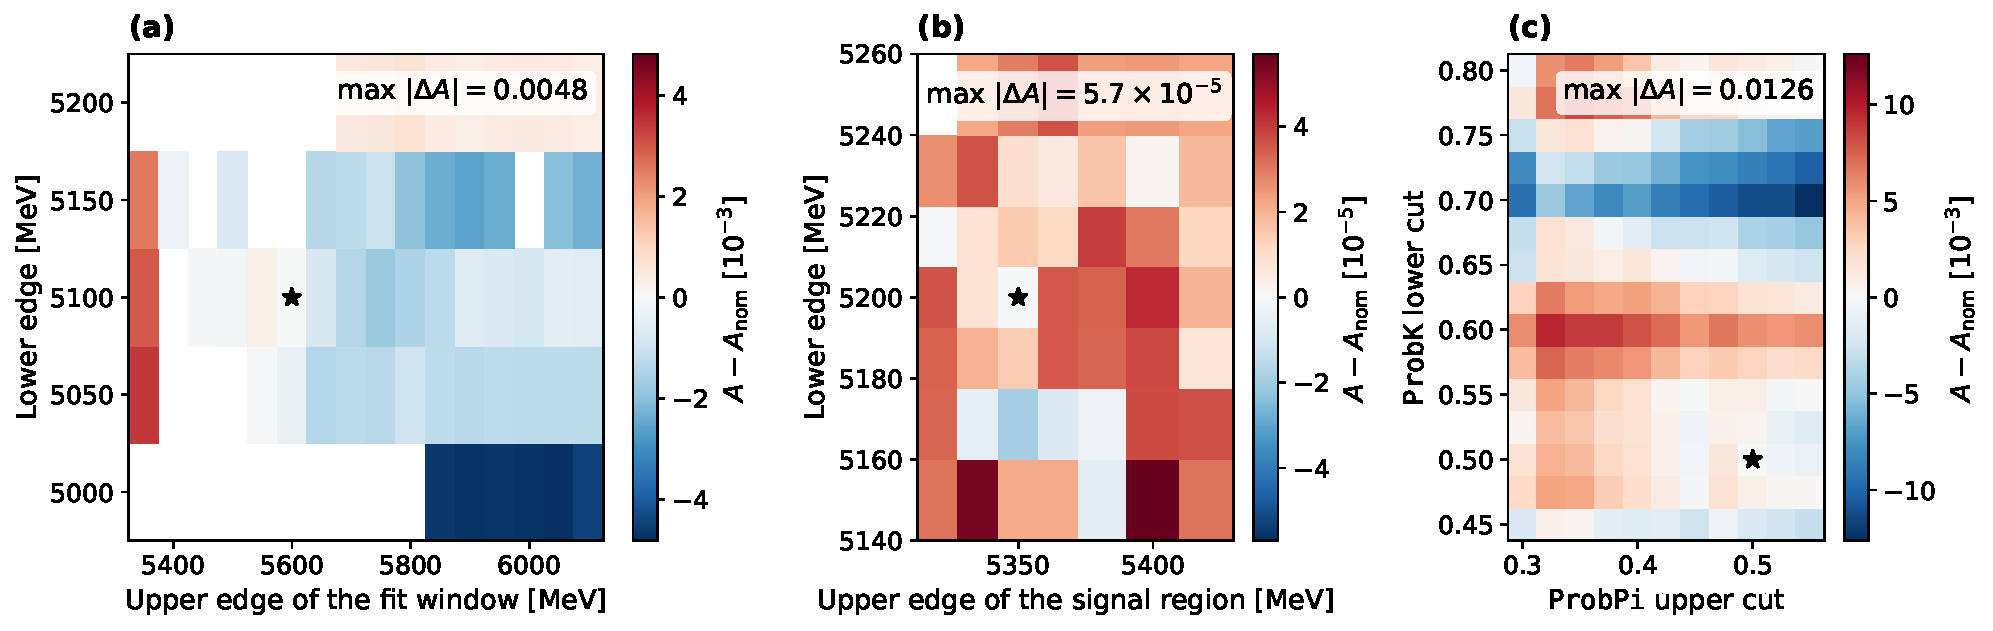
\includegraphics[width=0.95\textwidth]{figures/freq_stability.pdf}
\caption{Stability of the fitted $\Araw$ over the three grids: (a) lower and upper edge of the fit window (only fits with a valid minimum and an accurate covariance are shown); (b) lower and upper edge of the signal region; (c) lower cut on \texttt{ProbK} and upper cut on \texttt{ProbPi}. The colour is the shift with respect to the nominal fit (star), in units of $10^{-3}$ for (a) and (c) and $10^{-5}$ for (b); the statistical uncertainty of the nominal fit is $8.5\times10^{-3}$.}
\label{fig:freq_stability}
\end{figure*}

\subsection{All Fits of the Nominal Model and of Its Variants}
\label{sec:syst_tables}
\emph{In short: the Bayesian and Frequentist results of every variant and cross-check side by side.}

\subsection{Shifts of All Variants}
\label{app:syst_variants}
\emph{In short: the shifts of the Bayesian and Frequentist fits coincide variant by variant; the preselection group dominates, and the single exponential, rejected by the data, is drawn open.}
The $13$ variants of the systematic study (Sec.~\ref{sec:syst}) are shown in Fig.~\ref{fig:syst_variants}. For the variants that change the sample the bar is the expected statistical spread $\sigma_B$ of the shift (Sec.~\ref{sec:checks_barlow}); the others have no bar because the sample is the same. The Bayesian (purple) and Frequentist (green) shifts agree variant by variant, the preselection group is the largest, and the single exponential, which the data reject, is drawn open and excluded from the uncertainty.

\begin{figure}[t]
\centering
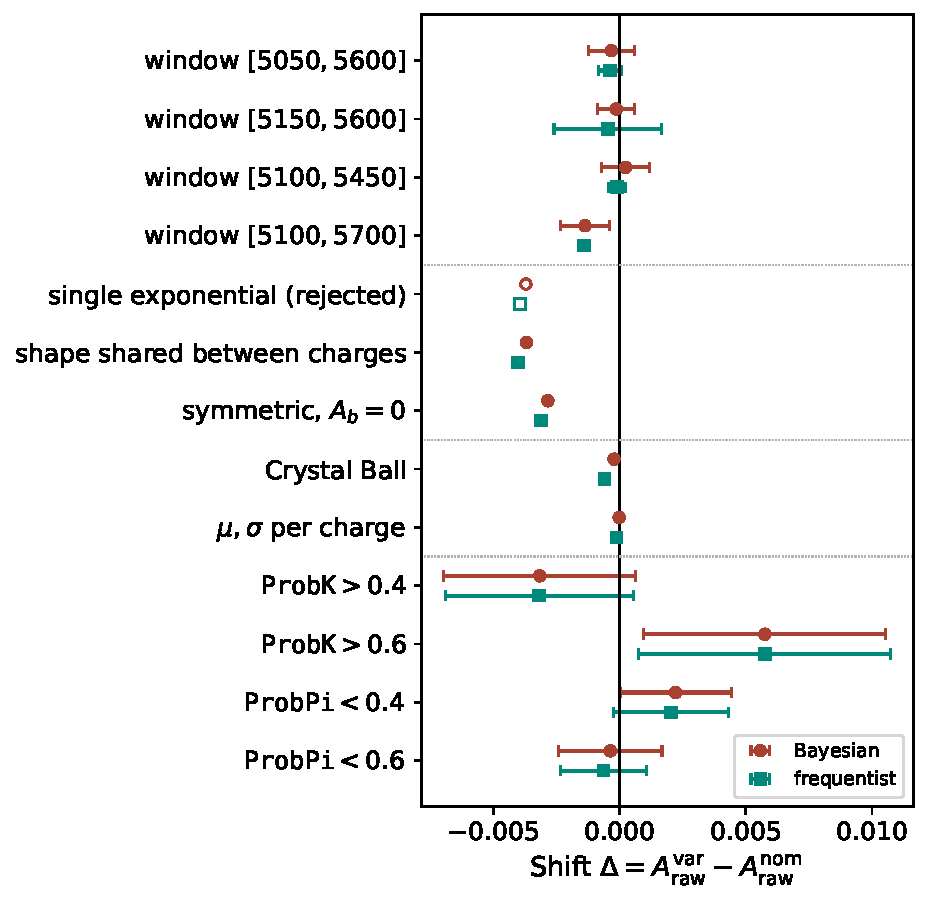
\includegraphics[width=\columnwidth]{figures/syst_variants.pdf}
\caption{Shift $\Delta=A_{\mathrm{raw}}^{\mathrm{var}}-A_{\mathrm{raw}}^{\mathrm{nom}}$ of every variant of the systematic study, Bayesian and Frequentist fits; bars: expected spread $\sigma_B$ of a nested subsample (variants that change the sample only). Open symbols: variant rejected by the data. The dotted lines separate the groups (window, background, signal, preselection).}
\label{fig:syst_variants}
\end{figure}

\subsection{Scan of the Particle-Identification Cuts}
\label{sec:syst_pid_scan}
\emph{In short: on the tight side the shift scatters around zero within $1.3\,\sigma_B$ and the pion requirement is flat; loosening $\texttt{ProbK}$ moves $\Araw$ monotonically, which supports the nominal requirement.}
A scan in steps of $0.05$ of each cut ($\texttt{ProbK}>0.30$--$0.85$, $\texttt{ProbPi}<0.15$--$0.70$) shows that on the tight side the shifts scatter around zero without a trend, all within $1.3\,\sigma_B$, and the pion requirement is flat: the $\texttt{ProbK}>0.6$ value is a statistical fluctuation and the preselection uncertainty is conservative. Loosening the kaon requirement moves $\Araw$ monotonically ($-0.0019$ to $-0.0111$ for $\texttt{ProbK}>0.45$--$0.30$, the last at $2.5\,\sigma_B$), as expected if misidentified $B\to K\pi\pi$ and $B\to\pi KK$ decays, not in the mass model, enter the sample; this supports the nominal requirement.
The scan is shown in Fig.~\ref{fig:syst_pid_scan}.

\begin{figure*}[!t]
\centering
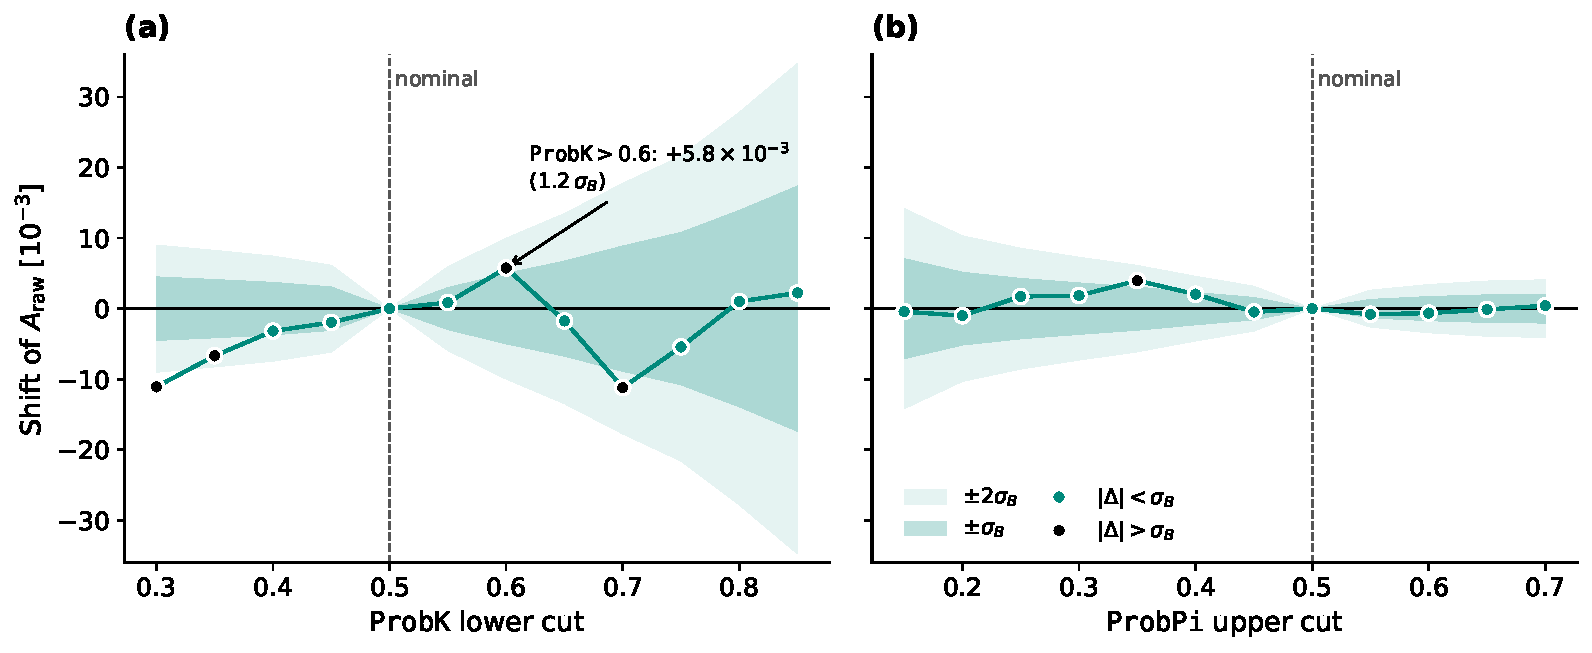
\includegraphics[width=0.85\textwidth]{figures/short_pid_scan.pdf}
\caption{Shift of $\Araw$ (Frequentist fit) as a function of (a) the $\mathtt{ProbK}$ lower cut and (b) the $\mathtt{ProbPi}$ upper cut, in steps of $0.05$, with the expected statistical spread of the nested sample ($\pm\sigma_B$ dark, $\pm2\sigma_B$ light); points beyond $\sigma_B$ are in red and the nominal cut is the dashed line. On the tight side of $\mathtt{ProbK}$ the points scatter around zero without trend and the pion requirement is flat; loosening $\mathtt{ProbK}$ moves $\Araw$ monotonically. The variant used in the systematic study, $\mathtt{ProbK}>0.6$, is a $1.2\,\sigma_B$ fluctuation.}
\label{fig:syst_pid_scan}
\end{figure*}

\subsection{Sensitivity of $\sigma_B$ to Differences between the Methods}
\emph{In short: $\sigma_B$ is the difference of two nearly equal uncertainties and is sensitive to small differences between the methods; a variant at the threshold can be classified differently without changing the result.}
Each method computes $\sigma_B$ from its own uncertainties (posterior standard deviation, Hesse error). Since $\sigma_B$ is the difference of two nearly equal uncertainties, it is sensitive to small differences between them, including the Monte Carlo noise of the posterior standard deviation (1--3\%), and a variant close to the threshold can be classified differently by the two methods: $\texttt{ProbPi}<0.4$ counts for the Bayesian fit ($|\Delta|=0.00223$, $\sigma_B=0.00220$) and not for the Frequentist one ($0.00204$ vs $0.00229$). This does not affect the result, since the uncertainty of each group is set by its largest shift, the same in both methods.
\subsection{Validation of the Rule for Nested Samples}
\label{sec:checks_barlow}
\emph{In short: the spread of the shift of $\hat A$ between a sample and its tighter-identification subsample is the one given by the quadrature difference of the uncertainties.}
The systematic study counts a variant that changes the sample only if its shift exceeds $\sigma_B=\sqrt{|\sigma_{\mathrm{var}}^2-\sigma_{\mathrm{nom}}^2|}$ (Sec.~\ref{sec:syst}). To verify the rule, $300$ bootstrap replicas of the nominal sample were fitted before and after the tighter selections $\texttt{ProbK}>0.6$ and $\texttt{ProbPi}<0.4$ (Fig.~\ref{fig:checks_barlow}): the standard deviation of the shift is $0.0051$ and $0.0025$, against median $\sigma_B$ of $0.0050$ and $0.0023$ (ratios $1.02$ and $1.09$), and the shifts follow a Gaussian of width $\sigma_B$. The mean shift of the replicas ($0.0060$ and $0.0020$) is that of the data, which is preserved by the resampling: it is a property of the sample and not a fluctuation of the rule.

\begin{figure*}[t]
\centering
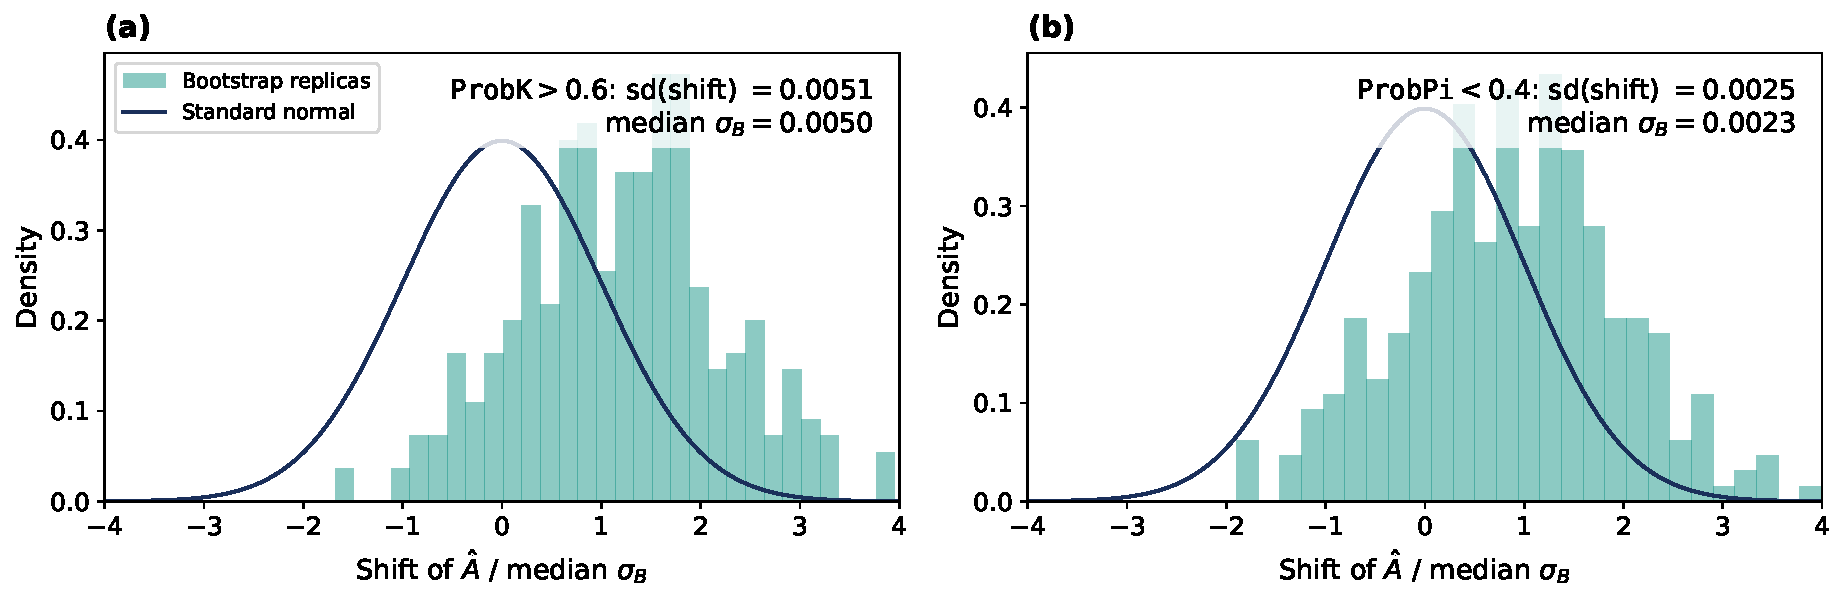
\includegraphics[width=0.95\textwidth]{figures/validation_barlow.pdf}
\caption{Shift of $\hat A$ between the nominal sample and a tighter selection, divided by the median $\sigma_B$, in $300$ bootstrap replicas of the data: (a) $\texttt{ProbK}>0.6$, (b) $\texttt{ProbPi}<0.4$, and standard normal distribution.}
\label{fig:checks_barlow}
\end{figure*}


\section{Validation of the Estimator and of the Intervals}
\label{sec:validation}
\label{app:ext_valid}
\emph{In short: toy-MC experiments generated from the fitted model show that the maximum-likelihood estimate of $A$ is unbiased and attains the minimum variance bound, that the Wilks interval has the nominal coverage, and that the test of $A=0$ has the expected size and a power that is known as a function of the injected asymmetry.}
The asymptotic properties of the maximum-likelihood estimator and of the profile-likelihood ratio were verified on toy-MC experiments generated from the fitted model (Sec.~\ref{sec:validation_toys}), which allow the true value of $A$ to be chosen.
\subsection{Generation of the Toy-MC Experiments}
\label{sec:validation_toys}
\emph{In short: toy experiments are generated from the fitted model (Poisson yields, masses by the transformation method) and fitted with the nominal procedure: $1000$ at the fitted value and $300$ at each of four other values of $A$.}
The Frequentist results of Sec.~\ref{sec:frequentist} rest on asymptotic properties of the maximum-likelihood estimator and of the profile-likelihood ratio, and Sec.~\ref{sec:freq_coverage} verified the coverage by resampling the data. Here the same questions are asked of toy-MC experiments generated from the fitted model, as was done for the Bayesian interval in Sec.~\ref{sec:bayes_toymc}, which allows the true value of $A$ to be chosen. The fitted model of Sec.~\ref{sec:model} defines the toy-MC datasets: for each charge the yields of signal and background are Poisson-fluctuated, the signal masses are drawn from the truncated Gaussian and the background masses from the two truncated exponentials by the transformation method. Each dataset is fitted with the nominal Frequentist procedure; the likelihood ratio $t(A_{\mathrm{true}})=-2\ln[L(A_{\mathrm{true}})/L(\hat A)]$ and the statistic of the test of $A=0$, $q(0)$, are computed with the other eleven parameters profiled. One thousand toy-MC experiments were generated at the fitted value, $A_{\mathrm{true}}=-0.0441$, and $300$ at each of $A_{\mathrm{true}}=-0.1$, $-0.02$, $0$ and $+0.05$; between $1\%$ and $3\%$ of the fits are not flagged as valid by \texttt{MIGRAD} and are excluded.
\subsection{Bias, Efficiency and Coverage}
\label{sec:validation_estimator}
\emph{In short: no bias larger than $0.0008$, an estimator spread equal to the Hesse uncertainty within $6\%$, and coverage of $0.70\pm0.01$ and $0.95\pm0.01$ at the fitted value; the test of $A=0$ has size $0.051\pm0.013$ and power $0.68$ at $A=-0.02$.}
Table~\ref{tab:validation_toys} summarizes the estimator over the five injected values: the bias of $\hat A$ is at most $0.0008$ ($1.6$ standard errors), its spread equals the mean Hesse uncertainty within $6\%$ and the pulls have width $0.94$--$1.05$, so the estimator is unbiased and reaches the minimum variance bound. At the fitted value the coverage of $t(A_{\mathrm{true}})\leq1$ is $0.696\pm0.015$ ($68.3\%$ level) and $0.954\pm0.007$ ($95.4\%$ level); at $A_{\mathrm{true}}=+0.05$ the $68\%$ coverage is $0.614\pm0.028$, $2.5$ standard deviations low, not unexpected among five values.

\begin{table}[h]
\centering
\resizebox{\ifdim\width>\linewidth\linewidth\else\width\fi}{!}{\begin{tabular}{rrcccc}
\toprule
$A_{\mathrm{true}}$ & $n$ & bias & sd$(\hat A)/\langle\sigma_{\mathrm{Hesse}}\rangle$ & cov.\ $68\%$ & cov.\ $95\%$ \\
\midrule
$-0.1$ & $297$ & $-0.0005\pm0.0005$ & $0.94$ & $0.71$ & $0.96$ \\
$-0.0441$ & $985$ & $-0.0001\pm0.0003$ & $0.97$ & $0.70$ & $0.95$ \\
$-0.02$ & $290$ & $-0.0008\pm0.0005$ & $1.02$ & $0.69$ & $0.94$ \\
$0$ & $293$ & $+0.0002\pm0.0005$ & $1.01$ & $0.69$ & $0.95$ \\
$+0.05$ & $293$ & $-0.0004\pm0.0005$ & $1.05$ & $0.61$ & $0.96$ \\
\bottomrule
\end{tabular}}
\caption{Toy-MC experiments at five injected values of the asymmetry: number of valid fits, bias of $\hat A$ with its standard error, spread of the estimates relative to the mean Hesse uncertainty ($0.0085$), and coverage of the intervals $t(A_{\mathrm{true}})\leq1$ and $\leq3.84$.}
\label{tab:validation_toys}
\end{table}

Together, the estimator is unbiased and efficient, the interval has its nominal coverage and the test its nominal size (Sec.~\ref{sec:validation_power}); the $5.2\sigma$ of the data is an extrapolation of the $\chi^2_1$ tail, which the $293$ experiments check only down to the $3\sigma$ level.
\subsection{Asymptotic Behavior of the Estimator}
\label{sec:checks_scaling}
\emph{In short: with the number of candidates the bias tends to zero, the spread scales as $N^{-1/2}$ and the distribution of $\hat A$ becomes Gaussian, as the central limit theorem and the asymptotic properties of the maximum-likelihood estimate predict.}
The $300$ toy-MC datasets for each size of the low-statistics study (Sec.~\ref{sec:bayes_lowstat}) show the approach to the asymptotic limit (Table~\ref{tab:checks_scaling}): the bias decreases from $-0.0085$ at $N=50$ to $+0.0009$ at $N=2000$, the product of the spread and $\sqrt N$ is constant, and the distribution of $\hat A$ is compatible with a Gaussian from $N=150$ (Shapiro-Wilk $p>0.3$), with a mild excess kurtosis at $N=50$ ($p=0.03$). Linear propagation of the Poisson uncertainty of the signal yield, $\sigma(A)=\sqrt{(1-A^2)/N_s}$ with $N_s=0.86\,N$, gives $0.153$ at $N=50$ and $0.024$ at $N=2000$, against spreads of $0.161$ and $0.023$: it is correct at the few-per-cent level, because the fit also has to determine the background, and the first-order expansion is not the limiting approximation. At the full sample the spread of the estimator equals the Hesse uncertainty (Sec.~\ref{sec:validation_estimator}).

\begin{table}[h]
\centering
\resizebox{\ifdim\width>\linewidth\linewidth\else\width\fi}{!}{\begin{tabular}{rcccccc}
\toprule
$N$ & bias & sd$(\hat A)$ & sd$\cdot\sqrt N$ & skewness & ex.\ kurtosis & Shapiro $p$ \\
\midrule
$50$ & $-0.0085$ & $0.1611$ & $1.14$ & $-0.15$ & $+0.64$ & $0.03$ \\
$150$ & $-0.0051$ & $0.0920$ & $1.13$ & $+0.16$ & $+0.31$ & $0.59$ \\
$500$ & $-0.0022$ & $0.0501$ & $1.12$ & $-0.08$ & $+0.38$ & $0.52$ \\
$2000$ & $+0.0009$ & $0.0225$ & $1.01$ & $-0.20$ & $-0.20$ & $0.32$ \\
\bottomrule
\end{tabular}}
\caption{Distribution of the maximum-likelihood estimate of $A$ in $300$ toy-MC datasets of $N$ candidates (six-parameter model of Sec.~\ref{sec:bayes_minimal}).}
\label{tab:checks_scaling}
\end{table}

\subsection{Size and Power of the Test of $A=0$}
\label{sec:validation_power}
\emph{In short: the test has the nominal size, the statistic $q(0)$ follows a $\chi^2$ distribution with one degree of freedom, and an asymmetry of $-0.02$ would be rejected at $3\sigma$ in one toy-MC experiment out of four.}
Under $A_{\mathrm{true}}=0$ the fraction of toy-MC experiments with $q(0)>3.84$ is $0.051\pm0.013$, against the nominal size $\alpha=0.05$, and $2$ of $293$ exceed $q=9$ ($3\sigma$), against the $0.8$ expected; the distribution of $q(0)$ is compatible with $\chi^2_1$ (Kolmogorov-Smirnov $p=0.79$, Fig.~\ref{fig:validation_null}a), and the tail used for the significance ($q=27$) is an extrapolation of it. The power, the probability of rejecting $A=0$ when the asymmetry is $A_{\mathrm{true}}$ (Fig.~\ref{fig:validation_injection}c), is $1.00$ at the fitted value and at $\pm$ the larger injected values, and $0.68$ ($0.27$ at $3\sigma$) at $A_{\mathrm{true}}=-0.02$: with $19{,}731$ candidates an asymmetry of $0.02$ is detected in about two experiments out of three at the $5\%$ size, and an asymmetry below that is not resolved.

\begin{figure*}[!t]
\centering
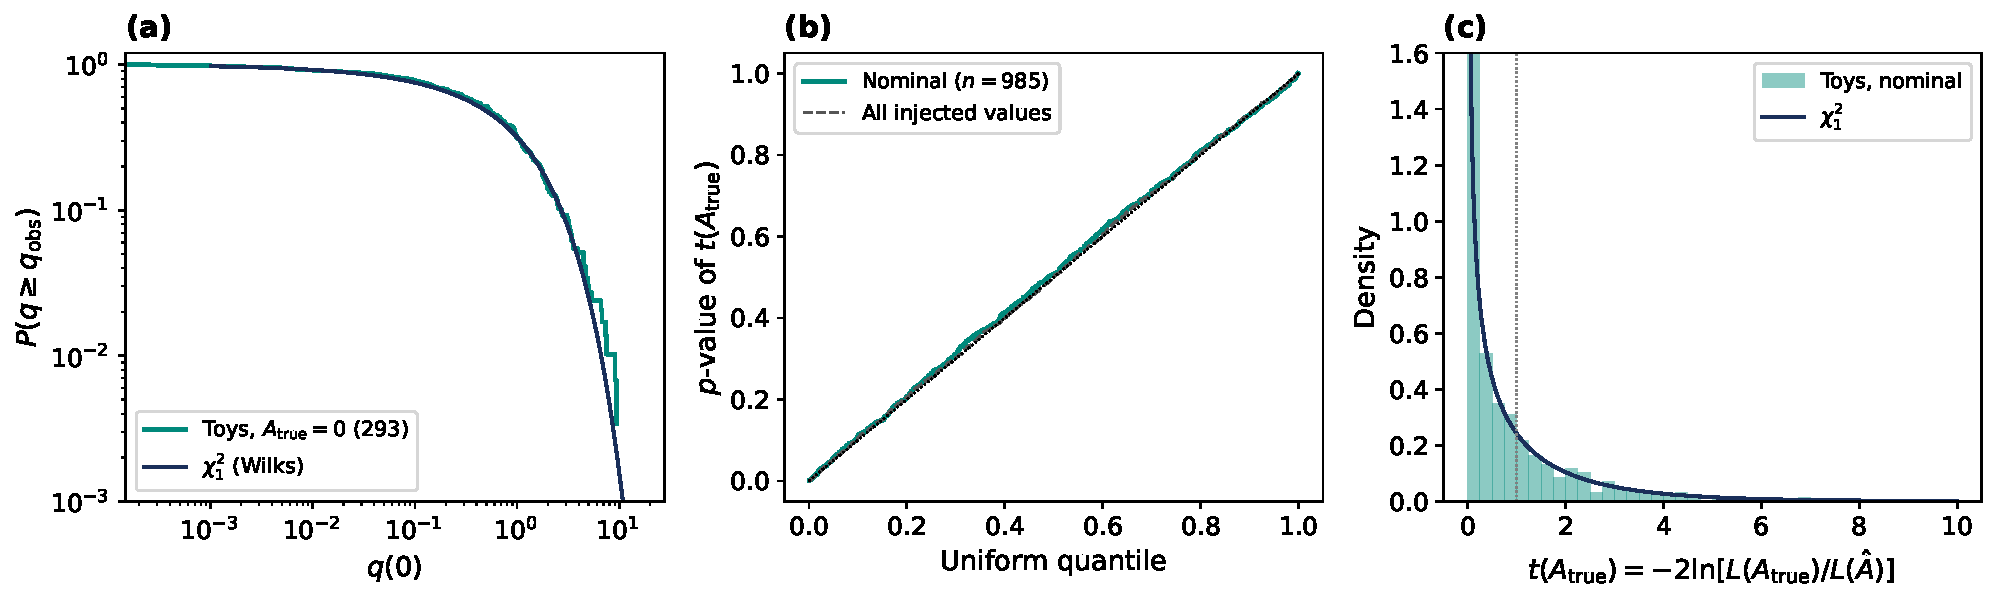
\includegraphics[width=0.95\textwidth]{figures/validation_null_wilks.pdf}
\caption{Toy-MC experiments, validity of Wilks' theorem. (a) Fraction of experiments with $q(0)$ above the observed value, for $A_{\mathrm{true}}=0$, compared with the $\chi^2_1$ distribution. (b) $p$-value of $t(A_{\mathrm{true}})$ against a uniform distribution, at the fitted value and pooled over the injected values. (c) Distribution of $t(A_{\mathrm{true}})$ at the fitted value and $\chi^2_1$.}
\label{fig:validation_null}
\end{figure*}

\begin{figure*}[!t]
\centering
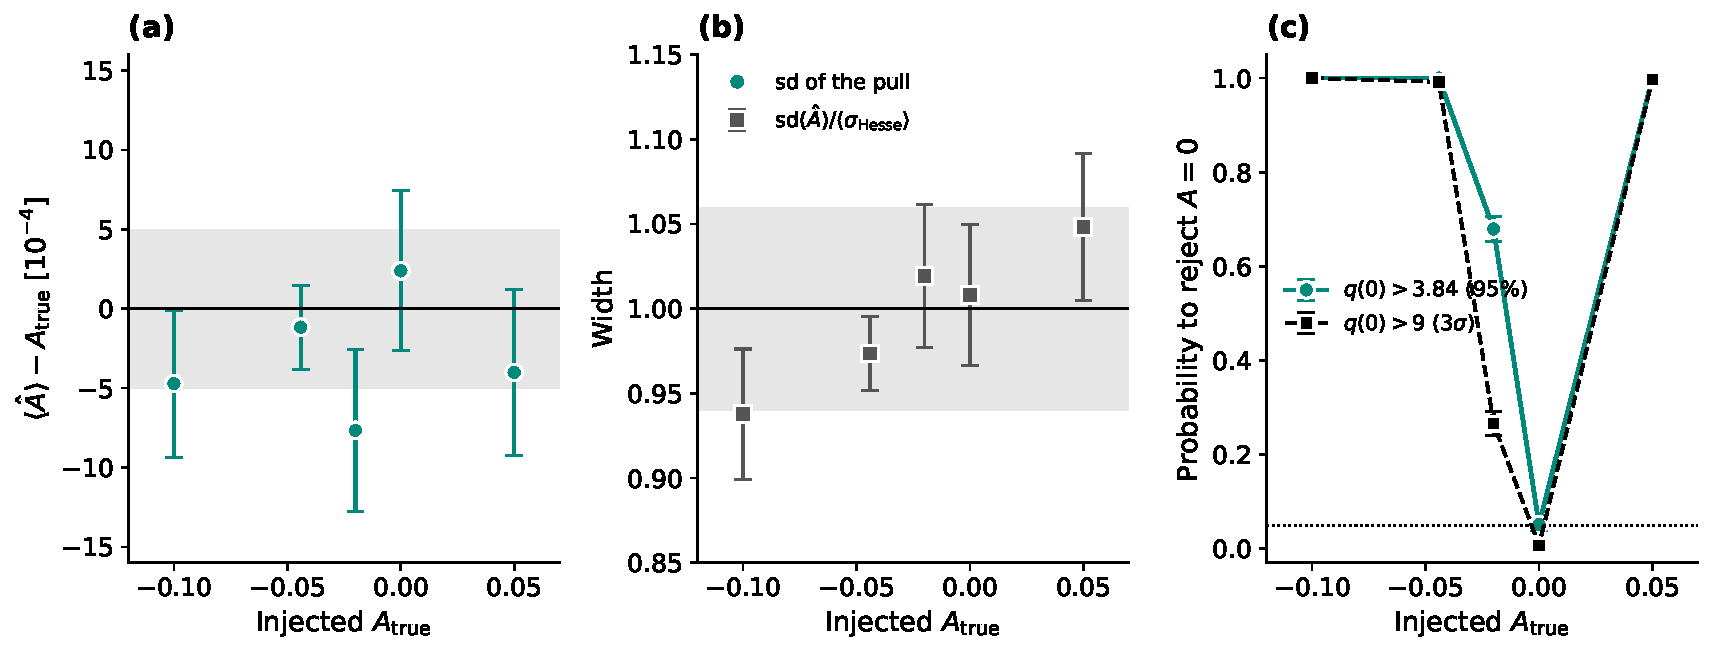
\includegraphics[width=0.95\textwidth]{figures/short_injection_power.pdf}
\caption{Toy-MC experiments at five injected asymmetries. (a) Bias of $\hat A$, with its standard error. (b) Spread of the estimates divided by the mean Hesse uncertainty, and width of the pulls. (c) Probability to reject $A=0$ in the test with $q(0)>3.84$ (size $5\%$) and $q(0)>9$ ($3\sigma$), as a function of the injected value: size at $A_{\mathrm{true}}=0$, power elsewhere.}
\label{fig:validation_injection}
\end{figure*}

\subsection{Goodness of Fit and the Binning}
\label{sec:validation_gof}
\emph{In short: the binned $\chi^2$ of toy-MC experiments follows its asymptotic distribution, so its $p$-values are accurate; the misfit of the data is $5.4$ standard deviations at $10\,\MeV$ bins and $2.0$ at $2.5\,\MeV$, because it lives on the scale of the flanks of the peak.}
The $p$-values of the binned $\chi^2$ rely on the asymptotic distribution with $\mathrm{ndof}$ degrees of freedom, which can fail for bins with few entries. The $\chi^2$ of $1000$ toy-MC experiments from the fitted model has mean $87.6$ and standard deviation $13.3$ for $2\times50$ bins ($88$ degrees of freedom, expected $\sqrt{2\cdot88}=13.3$), and mean $387.6$, standard deviation $27.1$ for $2\times200$ bins ($388$ degrees of freedom): the asymptotic $\chi^2$ distribution describes the toys (Fig.~\ref{fig:validation_gof}). The data give $159.5$ for $2\times50$ bins of $10\,\MeV$, $5.4$ standard deviations above the toys (asymptotic $p=4.8\times10^{-6}$, fewer than $1/1000$ toys above), $253.1/188$ for $5\,\MeV$ bins ($p=1.1\times10^{-3}$) and $441.7/388$ for $2.5\,\MeV$ bins ($2.0$ standard deviations, $p=0.031$, in toys $0.032$). The same fit therefore has $p=0.03$ or $p=5\times10^{-6}$ depending on the binning: the discrepancy between model and data is a feature of $\sim10\,\MeV$ width, the flanks of the peak (Fig.~\ref{fig:bayes_fit}), diluted in narrower bins, and the binned $\chi^2$ is a test whose power depends on the binning, in the same way as the Bayes factor depends on the prior width.

\begin{figure*}[!t]
\centering
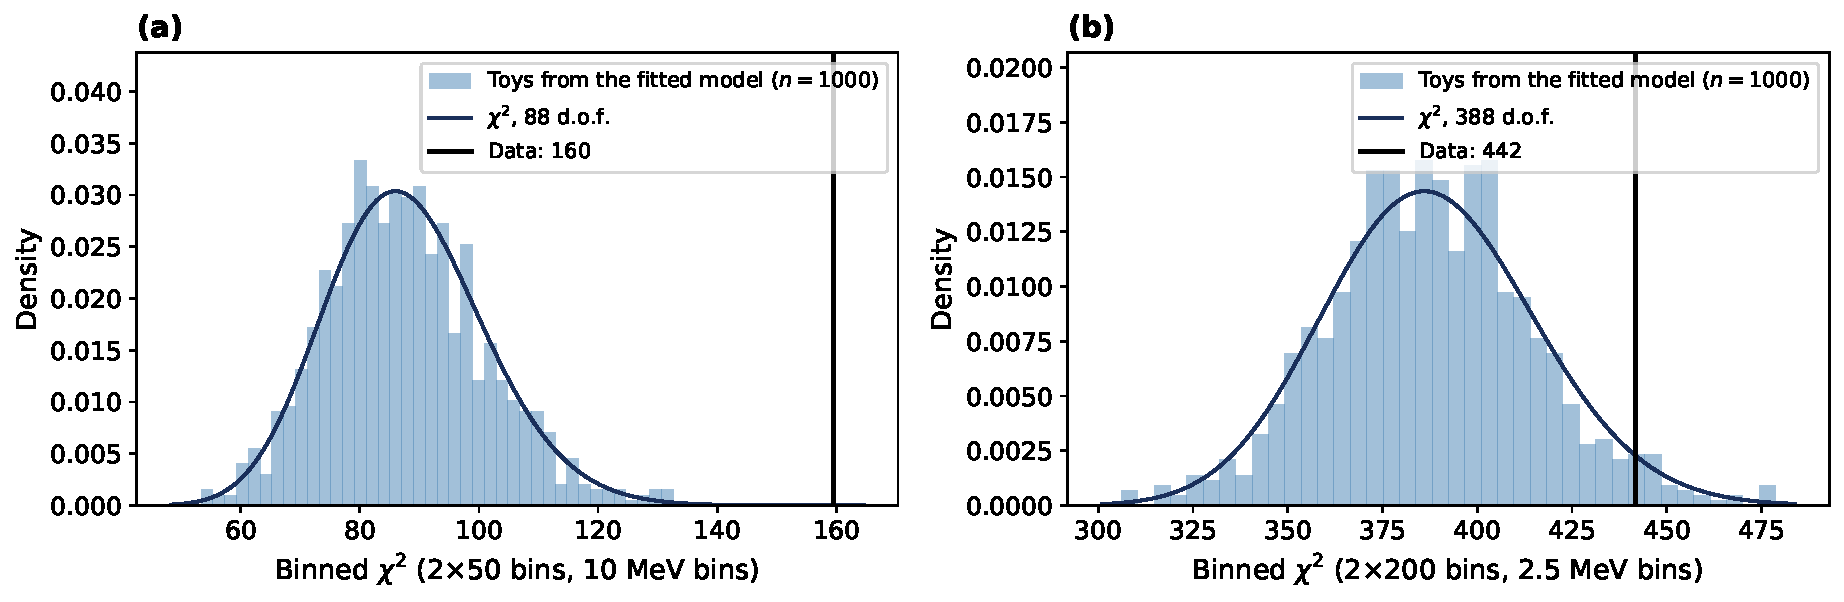
\includegraphics[width=0.95\textwidth]{figures/validation_gof_toys.pdf}
\caption{Binned $\chi^2$ of $1000$ toy-MC experiments from the fitted model, $\chi^2$ distribution with the corresponding degrees of freedom, and value of the data: (a) $2\times50$ bins of $10\,\MeV$, (b) $2\times200$ bins of $2.5\,\MeV$.}
\label{fig:validation_gof}
\end{figure*}

\FloatBarrier

\section{Local Asymmetry in the Dalitz Plane}
\label{sec:dalitz}
\label{app:ext_dalitz}
\label{sec:bayes_dalitz}
\emph{In short: the asymmetry is not uniform over the Dalitz plane ($\chi^2=80.8$ for $31$ degrees of freedom); it is concentrated at low $m^2_{\mathrm{lo}}$ outside the $\phi(1020)$ and, in the region of the published analysis of the same data, it reproduces the published value.}
To test whether the asymmetry is uniform over phase space or concentrated in specific regions, each candidate was placed in the Dalitz plane using the two opposite-sign $K^+K^-$ invariant masses $m^2(H1,H2)$ and $m^2(H1,H3)$ (Sec.~\ref{sec:data_presel}), sorted into $m^2_{\mathrm{lo}}$ and $m^2_{\mathrm{hi}}$ to remove the $H2/H3$ labeling ambiguity. The plane $[0,16]\times[0,30]\,\GeV^2$ in $(m^2_{\mathrm{lo}},m^2_{\mathrm{hi}})$ was divided into an $8\times8$ grid, fixed before looking at the asymmetries. In each bin with at least 20 candidates (32 of 64), the local asymmetry $A_i=(N_i^--N_i^+)/N_i$, with binomial uncertainty $\sigma(A_i)=\sqrt{(1-A_i^2)/N_i}$, was compared with the global counting asymmetry $A_{\mathrm{glob}}=-0.043$ through $S_i=(A_i-A_{\mathrm{glob}})/\sigma(A_i)$.

Figure~\ref{fig:bayes_dalitz} shows the occupancy of the bins (a), the local asymmetry (b) and its significance (c). The global homogeneity test, $\chi^2=\sum_iS_i^2=80.8$ for 31 degrees of freedom, holds in the signal window alone ($\chi^2=95.6/28$, signal purity $\approx$96\%), with the $D^0$ veto ($79.2/31$) and with all three charm vetoes ($74.4/31$), and for $6\times6$, $10\times10$ and $12\times12$ grids ($81.0/19$, $97.1/43$, $120.0/60$).

\begin{figure*}[t]
\centering
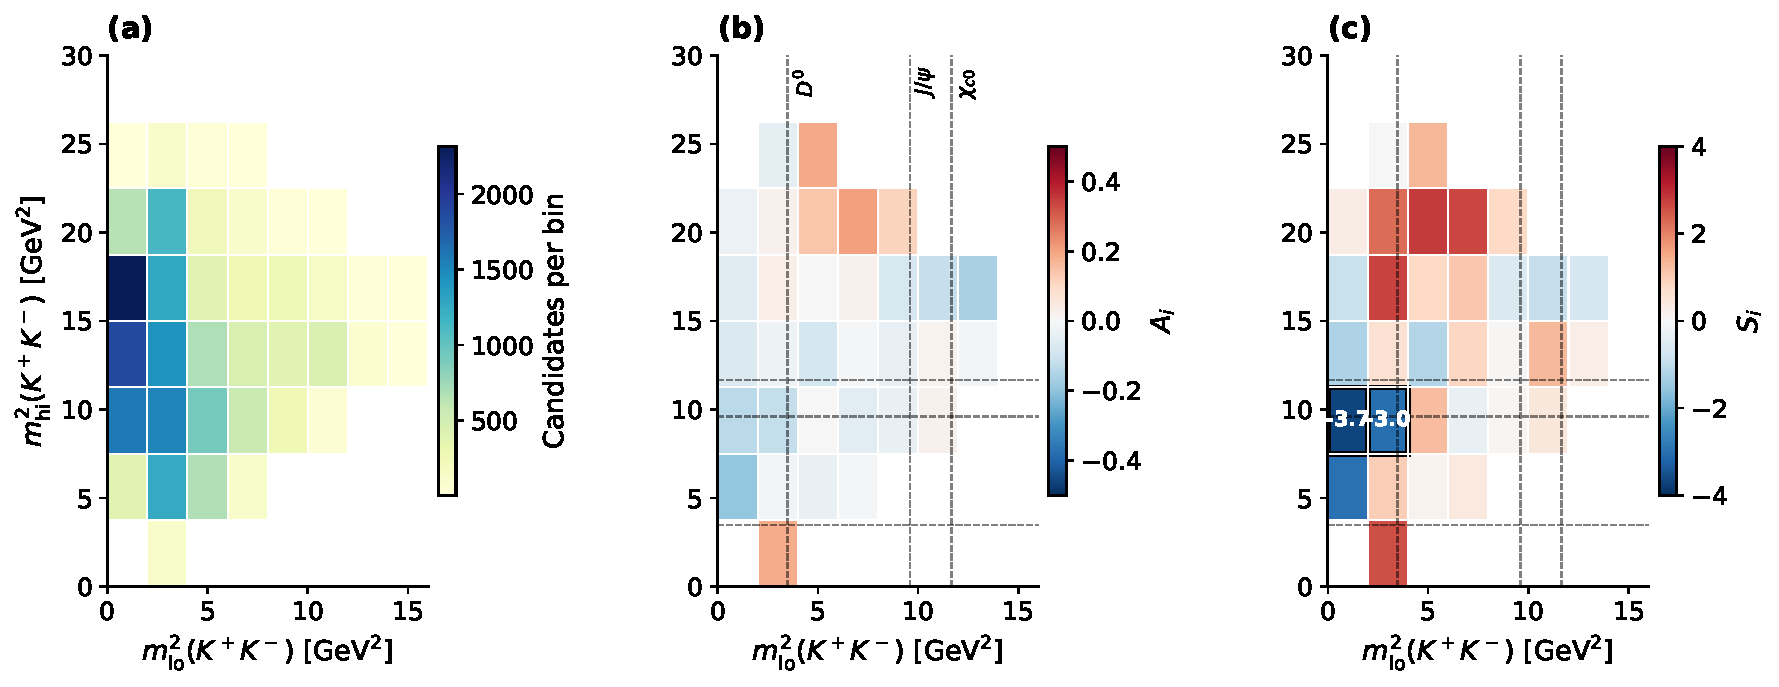
\includegraphics[width=0.95\textwidth]{figures/short_dalitz_maps.pdf}
\caption{Fixed $8\times8$ Dalitz-plot binning, all candidates in the fit window: (a) number of candidates per bin, (b) local asymmetry $A_i$ for bins with $\geq20$ candidates, and (c) local significance with respect to the global asymmetry, $(A_i-A_{\mathrm{glob}})/\sigma(A_i)$. The two bins with $|S_i|>3$ are outlined. Dashed lines: the squared masses of the $D^0$, $J/\psi$ and $\chi_{c0}$, in either opposite-sign pair.}
\label{fig:bayes_dalitz}
\end{figure*}

The structure does not depend on the magnet polarity either. The left-right part of the detection asymmetry changes sign when the polarity is reversed, so a local asymmetry produced by it would appear with opposite deviations in the two samples. In the region of the two significant bins ($m^2_{\mathrm{lo}}<4\,\GeV^2$, $7.5<m^2_{\mathrm{hi}}<11.25\,\GeV^2$) the counting asymmetry is $-0.129\pm0.023$ with the magnet down and $-0.126\pm0.028$ with the magnet up, although the global asymmetries of the two samples differ ($-0.051$ and $-0.032$), and the two maps agree bin by bin ($\chi^2=23.0$ for 29 bins, $p=0.78$). This split does not test the part of the detection asymmetry that does not change sign with the polarity, the different interaction of $K^+$ and $K^-$ with the detector material.
\subsection{Null Tests of the Local-Asymmetry Procedure}
\label{sec:dalitz_null}
\emph{In short: permuting the charges gives $\chi^2=31.5\pm8.4$, as expected, and never reaches the observed $80.8$; the phase-space simulation is consistent with no asymmetry, with slightly optimistic $\chi^2$ $p$-values.}
Two null tests check the procedure itself. Shuffling the charges among the candidates removes any local asymmetry while keeping the occupancy of the bins and the global asymmetry of the data: over $2000$ permutations the $8\times8$ grid gives $\chi^2=31.5\pm8.4$, as expected for 31 degrees of freedom, and no permutation reaches the observed value (permutation $p<5\times10^{-4}$; $p=1\times10^{-3}$ for the $12\times12$ grid). The phase-space simulation of the record, without asymmetry by construction, gives $\chi^2=40.0/30$ ($p=0.11$) with the same procedure on the whole sample; on $500$ subsamples of the size of the data the mean $\chi^2/\mathrm{ndof}$ is $1.16$ and $13\%$ have $p<0.05$, so the $\chi^2$ $p$-values are slightly optimistic (the binomial uncertainty is evaluated at the observed $A_i$). The permutation test, whose null distribution is exact, gives the same conclusion: the non-uniformity is a property of the data.
\subsection{Distribution of the Homogeneity Statistic under Charge Permutation}
\label{app:dalitz_perm}
\emph{In short: shuffling the charges reproduces the $\chi^2$ distribution of a uniform asymmetry, and the observed value lies far beyond all $2000$ permutations.}
For each of $2000$ random permutations of the charges among the candidates, which removes any local asymmetry while keeping the occupancy of the bins and the global asymmetry, the statistic $\chi^2=\sum_iS_i^2$ was computed on the $8\times8$ grid (Fig.~\ref{fig:dalitz_perm}). The distribution follows the $\chi^2$ with $31$ degrees of freedom, which confirms that the statistic is correctly normalized, and no permutation reaches the observed value ($80.8$).

\begin{figure}[t]
\centering
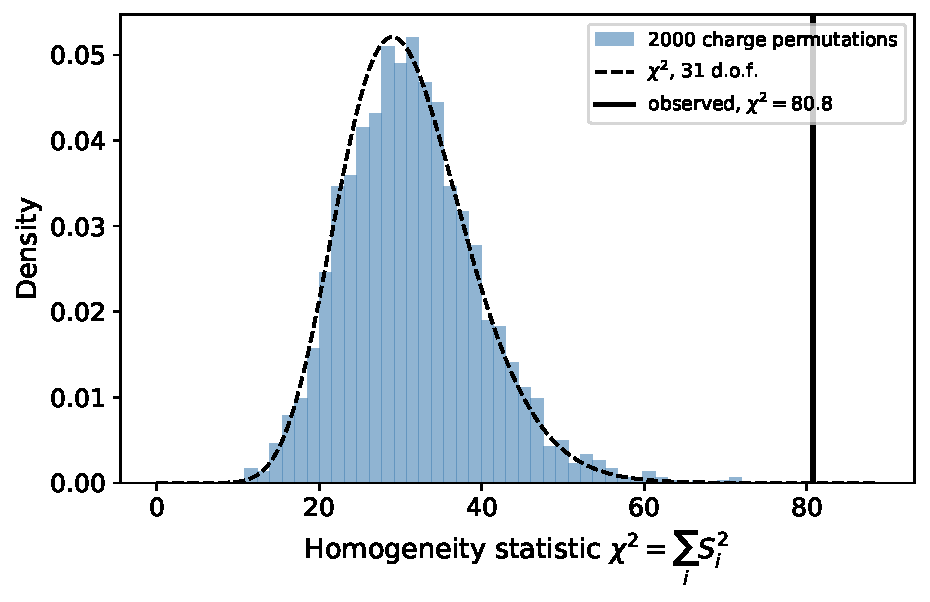
\includegraphics[width=\columnwidth]{figures/dalitz_permutation.pdf}
\caption{Homogeneity statistic $\chi^2=\sum_iS_i^2$ of the $8\times8$ Dalitz grid for $2000$ random permutations of the charges (histogram), $\chi^2$ distribution with $31$ degrees of freedom (dashed) and observed value (line).}
\label{fig:dalitz_perm}
\end{figure}

\subsection{Asymmetry in the $\phi(1020)$ Band and in the Significant Bins}
\label{app:dalitz_phi}
\emph{In short: the band of the $\phi(1020)$ has no asymmetry; the negative asymmetry is outside it, and larger when the $\phi$ candidates are removed.}
The asymmetry is not produced by the $\phi(1020)$ (Fig.~\ref{fig:dalitz_phi}). The band $|m_{\mathrm{lo}}-m_\phi|<10\,\MeV$ around the mass of the $\phi$ (panel~a) contains $1964$ candidates and has a counting asymmetry compatible with zero, $-0.004\pm0.023$, while the region of the two significant bins has $-0.128\pm0.018$ and, without the candidates of the $\phi$ band, $-0.145\pm0.019$; the $353$ candidates of the $\phi$ band that lie in that region have $+0.003\pm0.053$. The region just below the $\phi$ ($m^2_{\mathrm{lo}}<2\,\GeV^2$, outside the band) has $-0.120\pm0.014$ (panel~b).

\begin{figure*}[!t]
\centering
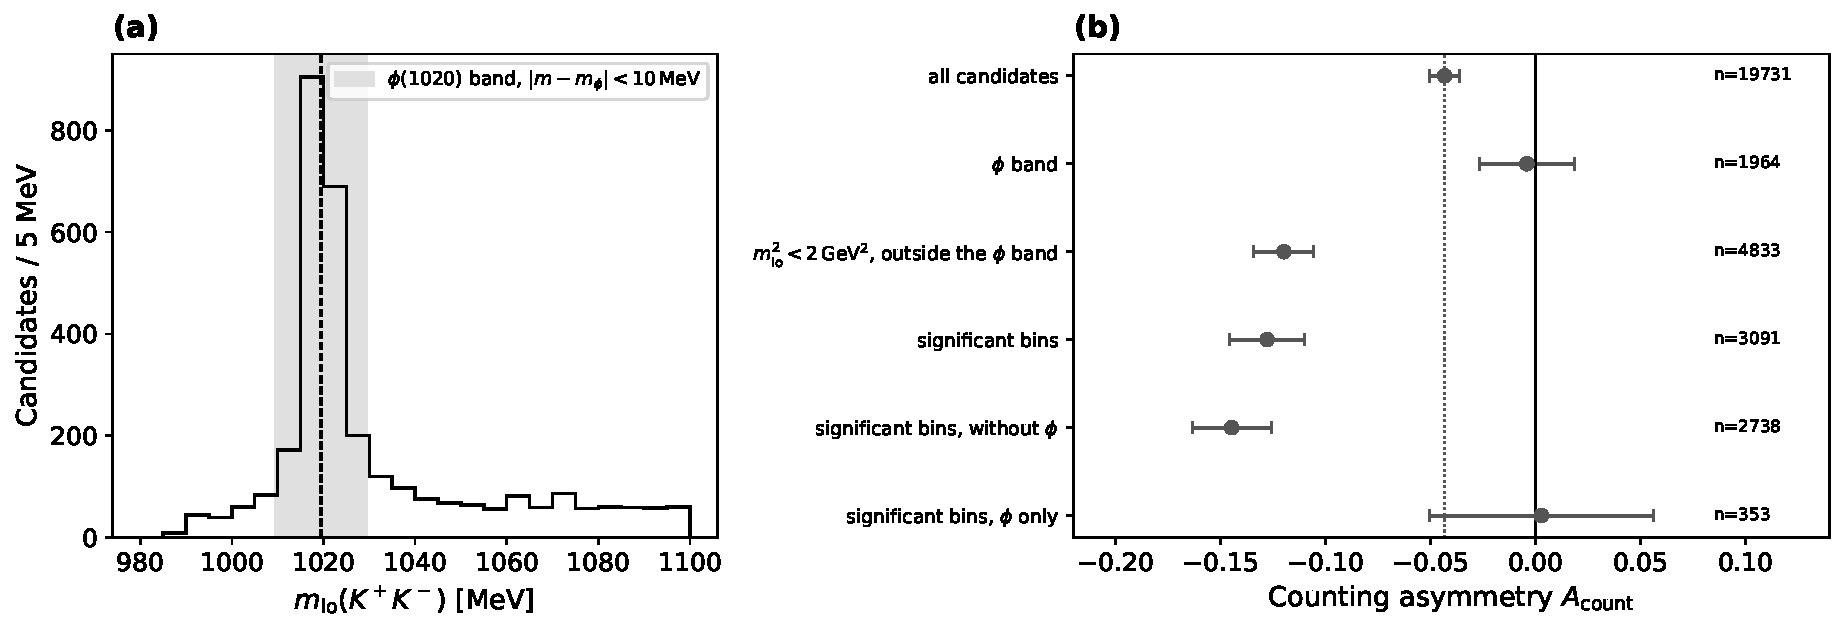
\includegraphics[width=0.9\textwidth]{figures/dalitz_phi_band.pdf}
\caption{(a) Distribution of $m_{\mathrm{lo}}(K^+K^-)$ around the $\phi(1020)$ ($5\,\MeV$ bins) and band used (shaded). (b) Counting asymmetry, with binomial uncertainty and number of candidates, of all candidates (dotted line), of the $\phi$ band, of the region $m^2_{\mathrm{lo}}<2\,\GeV^2$ outside the band, and of the two significant bins of Fig.~\ref{fig:bayes_dalitz}, with and without the candidates of the $\phi$ band, and of those candidates alone.}
\label{fig:dalitz_phi}
\end{figure*}


\section{Machine-Learning Analysis}
\label{sec:ml}
\emph{In short: classifiers trained on weak labels from the mass spectrum (there are no true labels) reach a test AUC of $0.86$; a cut on their score leaves $\Araw$ unchanged, and an adaptive partition of the Dalitz plane shows the same pattern as the fixed binning.}
As a complementary, data-driven approach to the signal/background separation of the mass fits (Secs.~\ref{sec:frequentist}--\ref{sec:bayesian}), supervised classifiers were trained on weak labels derived from the mass spectrum, and used to study whether an ML-assisted event selection changes $\Araw$ or the mass spectrum, and whether an adaptive partition of the Dalitz plane resolves local structure.
\subsection{Background: Regularization, Bias-Variance and Loss Functions}
\label{app:theory_ml}
\emph{In short: cross-entropy is a Bernoulli negative log-likelihood, $L1$ and $L2$ penalties shrink the coefficients, the test error splits into bias, variance and noise, and class weights rescale the score by a known factor.}
For a classifier with output probability $p(x)$ the binary cross-entropy $-\sum_i[y_i\ln p_i+(1-y_i)\ln(1-p_i)]$ is the negative log-likelihood of a Bernoulli distribution, the same principle (minimization of $-\ln L$) as in the mass fits; the Brier score $\frac1N\sum_i(p_i-y_i)^2$~\cite{brier} is the mean squared error of the predicted probability. The logistic regression is regularized by adding a penalty to the negative log-likelihood, $\alpha\sum_j\beta_j^2$ ($L2$, ridge: shrinks all the coefficients) or $\alpha\sum_j|\beta_j|$ ($L1$, lasso~\cite{tibshirani_lasso}: sets some of them exactly to zero), with $\alpha$ chosen by cross-validation (in \texttt{scikit-learn}, $C=1/\alpha$ multiplies the likelihood term). For squared error the expected test error of an estimator $\hat f$ decomposes as $E[(y-\hat f)^2]=\mathrm{Bias}^2+\mathrm{Var}+\sigma^2_{\mathrm{irr}}$: flexible models lower the bias and raise the variance, and the optimal complexity is where the sum is minimal, which the train-test gap of gradient boosting against the number of stages makes visible.
When the classes are weighted, with weight $w_c$ for class $c$, the minimized loss is $\sum_iw_{c_i}\ell_i$ and the classifier estimates $\tilde p=w_sp/(w_sp+w_b(1-p))$ instead of $p$. A monotonic recalibration (isotonic regression~\cite{zadrozny_elkan}) restores the probability scale without changing the ranking, hence the AUC.
\subsection{Background: Classification Without Labels}
\emph{In short: the classifier that is optimal between two mixtures of the same signal and background is monotonic in the signal-to-background ratio, so labels derived from the mass are sufficient.}
Let two samples be mixtures of the same signal and background densities $s(x)$ and $b(x)$, with signal fractions $f_1\neq f_2$. The ratio of their feature densities, $p_1(x)/p_2(x)=[f_1\,s+(1-f_1)\,b]/[f_2\,s+(1-f_2)\,b]$, is a monotonic function of $s(x)/b(x)$, so that the classifier that is optimal between the two mixtures is, up to a monotonic transformation, the one that is optimal between signal and background~\cite{cwola}. The proof requires that $s$ and $b$ be the same in the two samples, which is the condition discussed in Sec.~\ref{sec:ml_labels}.
\subsection{Background: Clustering and Uncertainty Estimators}
\emph{In short: $K$-means converges to a local minimum of the inertia, the adjusted Rand index measures the stability of a partition, and the spread of an ensemble estimates the epistemic uncertainty.}
$K$-means~\cite{lloyd_kmeans} alternates the assignment of each point to the nearest centroid and the update of the centroids to the cluster means; each step lowers the inertia $W$, so the algorithm converges to a local minimum that depends on the initialization (hence several random starts). The adjusted Rand index~\cite{hubert_ari} between two partitions is $(\mathrm{RI}-E[\mathrm{RI}])/(\max\mathrm{RI}-E[\mathrm{RI}])$: it is $1$ for identical partitions and $0$ on average for random ones, and it is used to quantify the stability of the partition under a change of the initialization. The spread of the predictions of an ensemble, $\sigma^2(x)=\frac1M\sum_m[p_m(x)-\bar p(x)]^2$, estimates the epistemic part of the uncertainty when the members differ in the training data (bootstrap, as in the Random Forest) or in the initialization (deep ensemble~\cite{deep_ensembles}), and MC dropout~\cite{gal_mcdropout} obtains $M$ such members from a single network by keeping the dropout active at inference.
\subsection{Weak Labels and Feature Set}
\label{sec:ml_labels}
\emph{In short: a classifier separates a signal-enriched window from the mass sidebands ($15{,}130$ signal-like and $1940$ background-like candidates, $20$ features, $60/20/20$ split); by the Neyman-Pearson argument of the CWoLa approach it is also the signal/background classifier, if the features carry no information on the mass.}
No candidate carries a true signal/background label, so the classifiers are trained with weak labels, following the classification-without-labels (CWoLa) approach~\cite{cwola}: a classifier is trained to separate two \emph{mixed} samples with different signal fractions, here a signal-enriched window around the $B$ peak and the mass sidebands. If, within each class, the feature distributions are the same in the two samples, the optimal classifier between the two mixtures is a monotonic function of the signal-to-background likelihood ratio $p_s(x)/p_b(x)$, which by the Neyman-Pearson lemma is the most powerful test statistic for signal against background: the classifier trained on the mixtures is also the optimal signal/background classifier~\cite{cwola}. Two conditions follow. The background in the sidebands must be representative of the background under the peak; and the features must not be correlated with the $B$ mass. The second condition cannot hold exactly: the reconstructed mass is not an input feature, but the nine momentum components of the three kaons determine it, so a flexible model can partly learn the mass, separate the two mass regions rather than signal from background, and \emph{sculpt} the mass distribution of the candidates that pass a cut on its score. Sec.~\ref{sec:ml_stability} tests this directly.
The labels use the nominal Bayesian fit (Sec.~\ref{sec:bayes_posterior}, $\mu=5284.39$, $\sigma=18.00\,\MeV$). Candidates with $|m-\mu|<2\sigma$, $m\in[5248.4,5320.4]\,\MeV$, are labeled signal-like ($15{,}130$); candidates in $[5150,\mu-4\sigma]\cup[\mu+4\sigma,5600]=[5150,5212.4]\cup[5356.4,5600]\,\MeV$ are labeled background-like ($1940$); the $2$--$4\sigma$ gap is left unlabeled. The region $5100$--$5150\,\MeV$, inside the fit window, is excluded from the background-like class to satisfy the first condition: there the background rises towards partially reconstructed $B$ decays (Sec.~\ref{sec:data_mass}), whose kinematics differ from those of the combinatorial background under the peak. The classes are imbalanced ($1940/15{,}130=0.128$). Every model is trained with the same balanced class weights, $w_c=N/(2N_c)$, i.e.\ $4.40$ for background-like and $0.56$ for signal-like candidates (through \texttt{class\_weight} for the scikit-learn models and the network, and through sample weights for gradient boosting), so that the two classes contribute equally to the loss. Figure~\ref{fig:ml_labels} shows the three regions on the mass spectrum. (Down-sampling the signal-like class and up-weighting it afterwards would have the same effect with less training data; the weights keep all candidates.)

\begin{figure}[h]
\centering
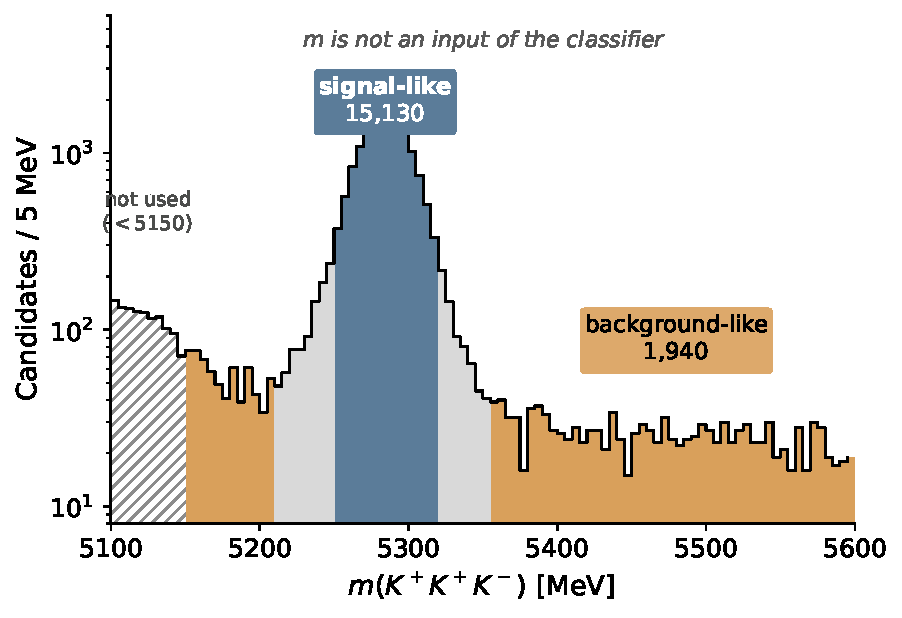
\includegraphics[width=\columnwidth]{figures/short_ml_labels.pdf}
\caption{Weak labels on the mass spectrum of the fit window: signal-like candidates ($|m-\mu|<2\sigma$, $15{,}130$) and background-like candidates (sidebands beyond $4\sigma$ and above $5150\,\MeV$, $1940$); the $2$--$4\sigma$ gap is left unlabeled and the region below $5150\,\MeV$, where the background rises towards partially reconstructed decays, is excluded.}
\label{fig:ml_labels}
\end{figure}

The feature set consists of the 6 per-track kinematic/PID variables (\texttt{PX}, \texttt{PY}, \texttt{PZ}, \texttt{ProbK}, \texttt{ProbPi}, \texttt{IPChi2}) for each of the 3 final-state tracks (18 features), plus two $B$-candidate variables not used in the preselection: \texttt{B\_FlightDistance} and \texttt{B\_VertexChi2}, standard discriminants against combinatorial background (a genuine $B$ flies further before decaying and has a better-reconstructed vertex than a random track combination). Both separate the weak-label classes (Kolmogorov-Smirnov $p<10^{-60}$) and are not redundant with the per-track features (Spearman $|\rho|\leq0.53$ with each of the 18), giving $20$ features. A principal-component analysis of the standardized features needs $15$ of $20$ components to reach $90\%$ of the variance, so no dimensionality reduction is applied; with $20$ features and $\sim10^4$ training candidates the sample is not in the regime where the distance-based methods suffer from the curse of dimensionality. The labeled sample was split $60/20/20$ into training, validation and test sets ($10{,}242/3414/3414$ candidates, $388$ background-like in the test set), stratified on the label, with the feature scaler fit on the training set only.
\subsection{Model Comparison}
\label{sec:ml_models}
\emph{In short: six classifiers; the tree ensembles and the neural network reach test AUC $0.857$--$0.864$, about $0.09$ above the linear models and indistinguishable from each other within the test-set uncertainty ($0.012$); gradient boosting, best in cross-validation, is the reference.}

Six classifiers were trained: logistic regression, without and with an $L1$ penalty (linear baselines), a decision tree (depth 4, fixed in advance as a shallow, interpretable baseline and not pruned), a Random Forest~\cite{breiman_rf} (300 trees of depth 8), gradient boosting~\cite{friedman_gbm} (200 stages of depth-3 trees, learning rate $0.05$), and a feed-forward neural network (FFNN: two hidden layers of 32 and 16 units with ReLU activation, dropout $0.2$, binary cross-entropy, the Adam optimizer~\cite{adam} with learning rate $10^{-3}$, early stopping on the validation AUC, sigmoid output). The linear models and the network are parametric, with a fixed number of parameters, and the trees and ensembles non-parametric, whose complexity grows with the data; the more flexible models are less interpretable, which is why the linear and single-tree baselines are kept. Both the logistic-regression log-loss and the network's binary cross-entropy are the negative log-likelihood of a Bernoulli distribution with probability $p(x)$, the same quantity minimized by the mass fits. The models are compared through the area under the receiver operating characteristic (ROC) curve (AUC), which equals the probability that a randomly chosen signal-like candidate receives a higher score than a randomly chosen background-like one ($0.5$ for a random classifier, $1$ for a perfect one). Table~\ref{tab:ml_models} gives the 5-fold cross-validated AUC on the training set and the AUC on the untouched test set, with its bootstrap uncertainty. The reference model for the rest of the section was chosen on the cross-validated AUC, so that the test set is not used for any choice: gradient boosting ($0.866$), essentially tied with the Random Forest ($0.863$).

\begin{table}[h]
\centering
\begin{tabular}{lccc}
\toprule
Model & CV AUC & Test AUC & Brier \\
\midrule
Logistic Regression       & $0.769 \pm 0.016$ & $0.771 \pm 0.013$ & $0.197$ \\
Logistic Regression (L1)  & --                & $0.771 \pm 0.013$ & $0.198$ \\
Decision Tree             & $0.816 \pm 0.011$ & $0.824 \pm 0.013$ & $0.133$ \\
Random Forest             & $0.863 \pm 0.017$ & $0.860 \pm 0.012$ & $0.122$ \\
Gradient Boosting         & $\mathbf{0.866 \pm 0.016}$ & $0.864 \pm 0.012$ & $0.116$ \\
FFNN                      & --                & $0.857 \pm 0.012$ & $0.134$ \\
\bottomrule
\end{tabular}
\caption{Cross-validated AUC (mean and standard deviation over the folds), test-set AUC (with bootstrap uncertainty) and test-set Brier score of the raw scores. Gradient boosting, best in cross-validation, is the reference model. The FFNN is validated on the validation set instead of by cross-validation.}
\label{tab:ml_models}
\end{table}

The three non-linear ensembles and the FFNN improve the AUC by $\sim$0.09 over the linear models and by $\sim$0.04 over the single tree (Fig.~\ref{fig:ml_roc}), while their mutual differences ($\leq0.007$) are smaller than the test-set uncertainty ($0.012$). The FFNN training is reproducible (fixed seeds, deterministic operations); its dependence on the random initialization, measured by retraining it with ten seeds, is $0.854\pm0.005$ in test AUC.

\begin{figure*}[t]
\centering
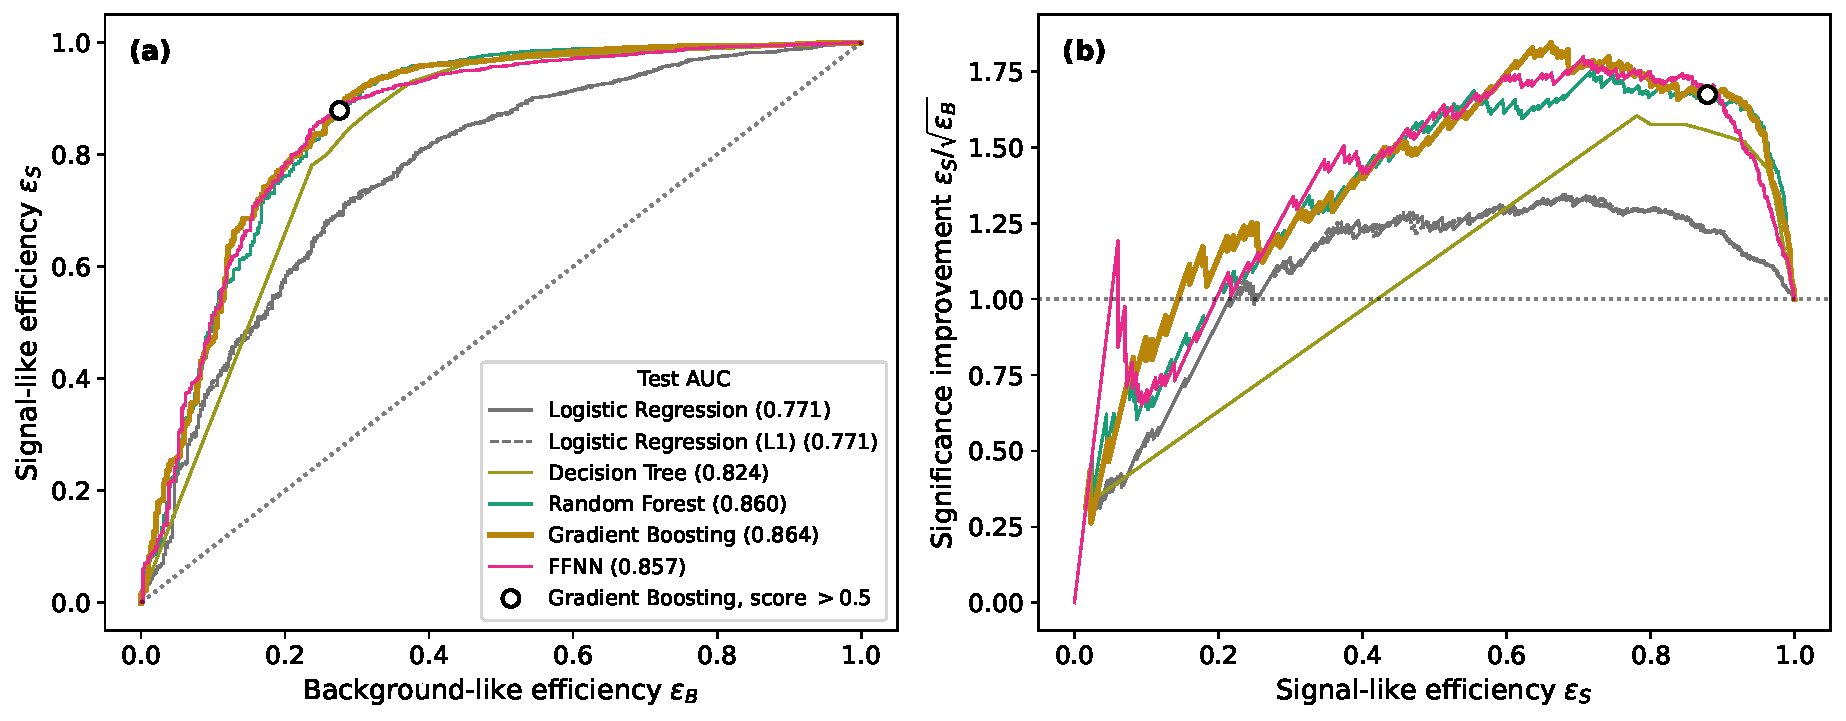
\includegraphics[width=0.95\textwidth]{figures/ml_nominal_roc.pdf}
\caption{Test-set performance of the classifiers: (a) ROC curves, with the test AUC of each model in the legend (Table~\ref{tab:ml_models}); (b) significance improvement $\varepsilon_S/\sqrt{\varepsilon_B}$ of a cut on the score as a function of the signal-like efficiency, where $1$ is no selection and $\varepsilon_{S,B}$ are the fractions of signal-like and background-like candidates kept. The reference model is drawn thicker, and the two logistic regressions overlap. The circle marks the cut on the reference score used in Sec.~\ref{sec:ml_stability}.}
\label{fig:ml_roc}
\end{figure*}

The two measures of the relevance of a feature available here -- the Random Forest importance (the decrease in Gini impurity $G=1-\sum_c p_c^2$, $p_c$ the class fractions in a node, produced by the splits on that feature) and the magnitude of the $L1$-regularized (Lasso~\cite{tibshirani_lasso}) logistic-regression coefficient of the standardized feature -- agree only partly (Fig.~\ref{fig:ml_features}; Spearman correlation of the two rankings $0.42$, $p=0.06$). The impact-parameter variables \texttt{IPChi2} dominate the Random Forest, while the Lasso coefficients are largest for \texttt{B\_FlightDistance}, \texttt{H3\_IPChi2}, \texttt{H2\_PZ} and \texttt{B\_VertexChi2}. The difference is expected: the Gini importance reflects the use of a feature in non-linear splits and interactions, and is shared among correlated features, while a linear coefficient measures the effect of a feature with the others held fixed. Both measures rank the two $B$-candidate variables among the top five (Random Forest 4th and 5th, Lasso 1st and 4th): they summarize in one number the displaced-vertex topology that the per-track variables encode only jointly.

\begin{figure*}[t]
\centering
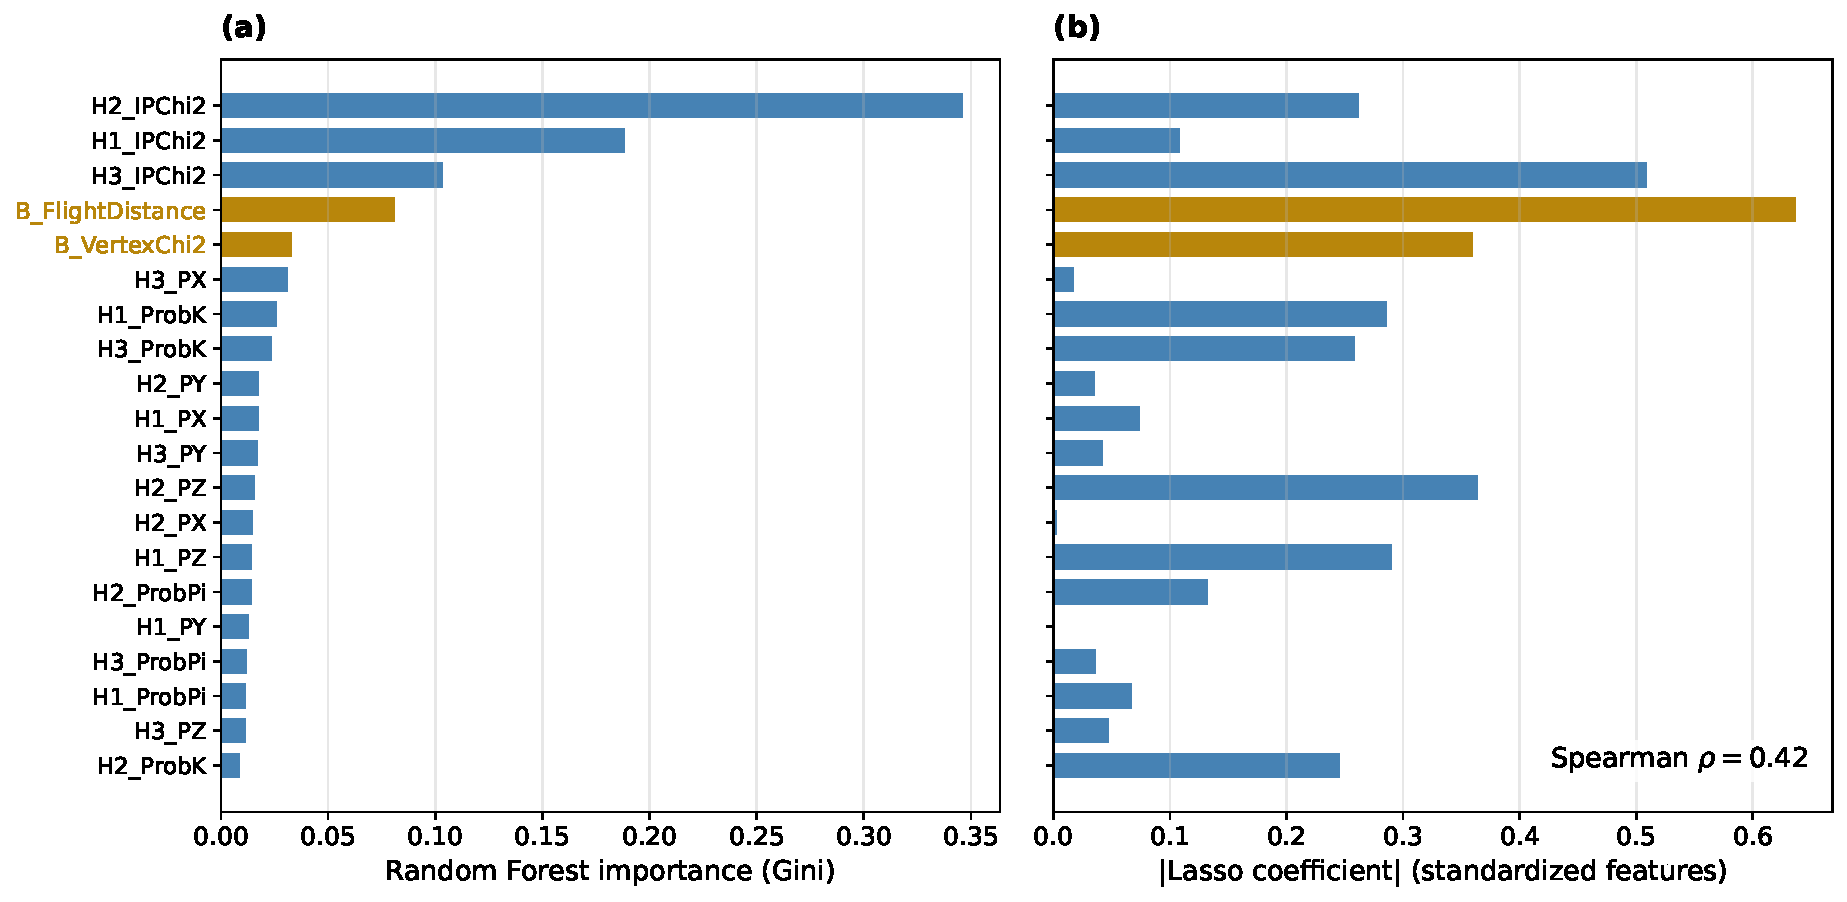
\includegraphics[width=0.95\textwidth]{figures/ml_nominal_features.pdf}
\caption{Random Forest feature importance (Gini, a) and magnitude of the Lasso coefficient of the standardized feature (b) for the 20 features, both ordered by Random Forest importance; the two $B$-candidate variables are highlighted.}
\label{fig:ml_features}
\end{figure*}

\subsection{Regularization, Bias-Variance, and Calibration}
\label{sec:ml_regcal}
\emph{In short: the linear model does not overfit, gradient boosting overfits beyond $\sim$150 stages without losing test AUC, and class weights bias the probabilities, which an isotonic recalibration corrects (Brier score $0.122\to0.062$) without changing the ranking.}
A scan of the regularization strength of the logistic regression (penalties and loss functions are defined in Sec.~\ref{app:theory_ml}) ($30$ log-spaced values of $C=1/\alpha$, cross-validated) gives the same optimal AUC for the $L1$ and $L2$ penalties ($0.7686$, at $C_{L1}=0.12$ and $C_{L2}=9.2$), and the optimal $L1$ penalty sets no coefficient to zero: the linear model does not overfit, and its limitation is the linear decision boundary, not the variance (Fig.~\ref{fig:ml_regularization}). The two curves differ only at strong regularization: the $L_2$ model, whose coefficients are shrunk but not removed, is flat over the whole range, while the $L_1$ model loses $\sim0.2$ of AUC for $C\lesssim3\times10^{-3}$, where its coefficients are set to zero.

\begin{figure}[h]
\centering
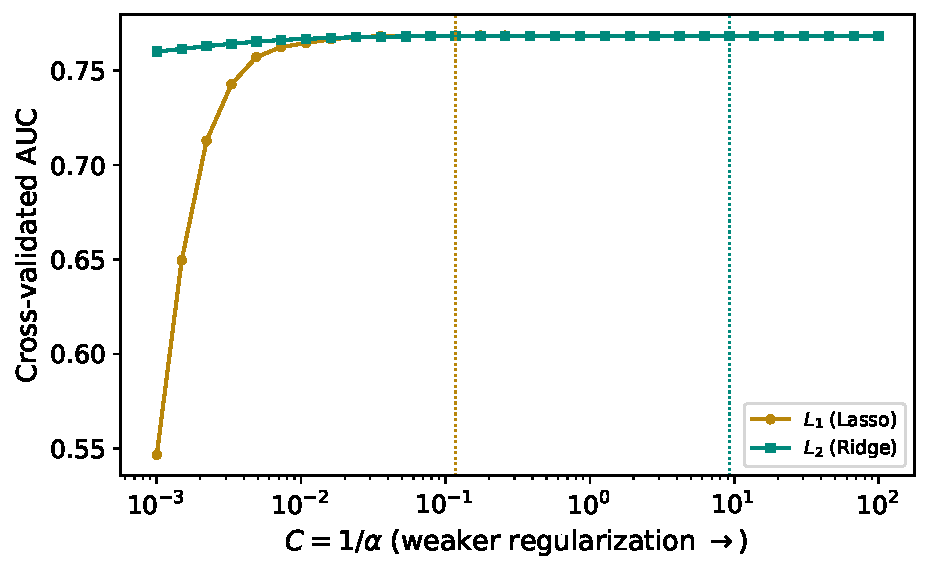
\includegraphics[width=\columnwidth]{figures/ml_regularization.pdf}
\caption{Cross-validated AUC of the logistic regression against the inverse regularization strength $C=1/\alpha$ ($30$ log-spaced values), for the $L_1$ (Lasso) and $L_2$ (Ridge) penalties; the dotted lines mark the optimum of each.}
\label{fig:ml_regularization}
\end{figure}

The bias-variance trade-off was studied with gradient boosting, whose complexity grows with the number of boosting stages (Fig.~\ref{fig:ml_bias_variance}). The test AUC rises up to $\sim$150 stages and then stays at $0.865$, while the training AUC keeps rising: the train-test gap grows from $0.018$ at 20 stages to $0.084$ at 300. The additional stages fit fluctuations of the training sample without improving the ranking of new candidates -- overfitting, which the default 200 stages of Table~\ref{tab:ml_models} do not reach in the test AUC. The test accuracy at the $0.5$ threshold stays below that of always predicting the majority class ($0.886$): with balanced class weights the classifier is trained to minimize the weighted error, in which a misclassified background-like candidate counts eight times more than a signal-like one, and not the unweighted error rate.

\begin{figure*}[t]
\centering
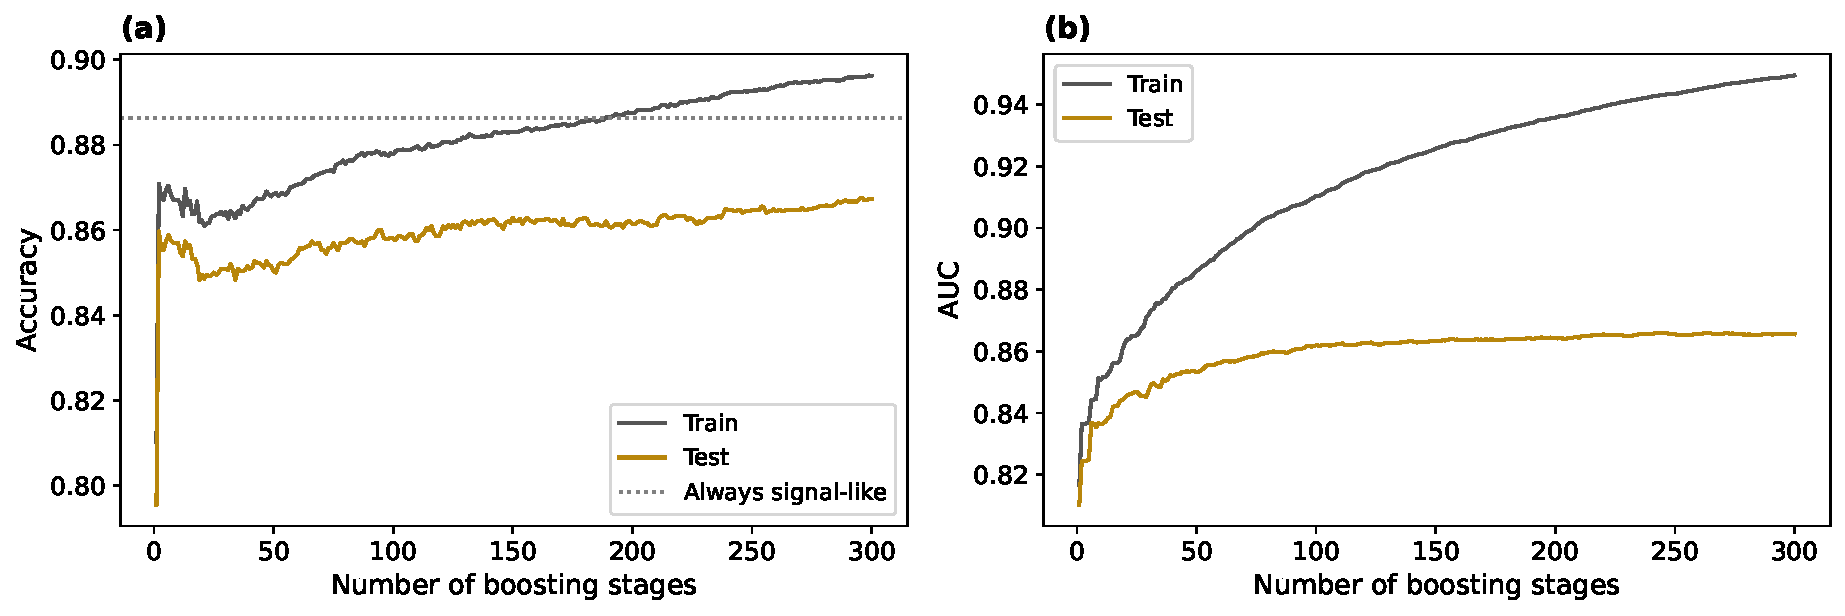
\includegraphics[width=0.95\textwidth]{figures/ml_nominal_bias_variance.pdf}
\caption{Gradient boosting: (a) accuracy at the $0.5$ threshold and (b) AUC on the training and test sets as a function of the number of boosting stages. The dotted line is the accuracy of always predicting the signal-like class.}
\label{fig:ml_bias_variance}
\end{figure*}

The AUC depends only on the ranking of the scores; whether a score can be read as a probability is measured by the Brier score~\cite{brier}, $\mathrm{BS}=\frac{1}{N}\sum_i (p_i-y_i)^2$, the mean squared difference between predicted probability $p_i$ and label $y_i\in\{0,1\}$ (lower is better). Class weights change the probabilities a model learns: a classifier trained with weights $w_s,w_b$ on the two classes converges to
\[
\tilde p=\frac{w_s p}{w_s p+w_b(1-p)}
\]
instead of the true $p$, i.e.\ it describes a world in which the classes are re-balanced. With $w_b>w_s$ the raw scores therefore \emph{underestimate} the probability of the signal-like class, which is what the reliability diagram of the Random Forest shows (Fig.~\ref{fig:ml_calibration}): at a raw score of $0.25$ the observed signal-like fraction is already $0.58$. An isotonic recalibration~\cite{zadrozny_elkan}, fitted on held-out folds of the unweighted training sample, follows the diagonal and halves the Brier score, from $0.122$ to $0.062$ (the Brier score is the mean squared error of the predicted probability against the $0/1$ label). Most of the gain undoes the re-weighting rather than correcting the model; the ranking, and hence the AUC and any selection based on a score threshold, is unchanged by a monotonic recalibration.

\begin{figure}[t]
\centering
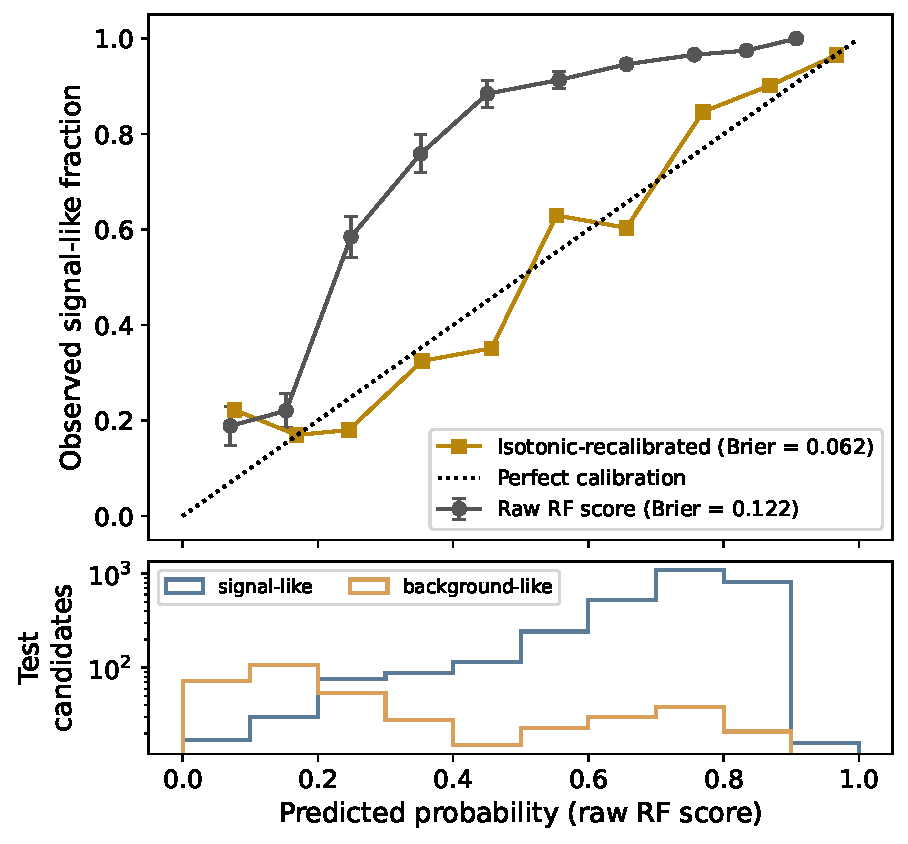
\includegraphics[width=\columnwidth]{figures/ml_nominal_calibration.pdf}
\caption{Reliability diagram of the Random Forest on the test set: observed fraction of signal-like candidates vs.\ predicted probability, for the raw score (with binomial uncertainties) and for the isotonic-recalibrated one. Bottom: distribution of the raw score for the two weak-label classes; the low-probability bins contain few candidates.}
\label{fig:ml_calibration}
\end{figure}

\subsection{Uncertainty Quantification}
\label{sec:ml_uncertainty}
\emph{In short: the three estimators give mean per-candidate uncertainties of $0.178$ (Random Forest), $0.095$ (MC dropout) and $0.050$ (deep ensemble); they measure different sources of variability, and only the Random Forest spread visibly decreases with the training-set size.}

The uncertainty of a prediction has two components: \emph{aleatoric}, from the intrinsic overlap of the classes in feature space, which more training data cannot reduce, and \emph{epistemic}, from the limited knowledge of the model parameters, which more training data reduces. Three estimators were compared, each giving an ensemble of $M$ predictions $p_m(x)$ for each candidate and quoting their spread, $\sigma(x)=\big[\frac1M\sum_m (p_m(x)-\bar p(x))^2\big]^{1/2}$: the $M=300$ trees of the Random Forest, each trained on a bootstrap sample; $M=300$ forward passes of the FFNN with dropout kept active at inference (MC dropout), which approximates sampling from a Bayesian posterior over the network weights~\cite{gal_mcdropout} (a full Bayesian network trained by variational inference was not used: it needs a dedicated implementation and MC dropout gives the same kind of ensemble at no extra cost); and a deep ensemble~\cite{deep_ensembles} of $M=10$ FFNNs trained from different random initializations. The mean per-candidate uncertainty is $0.178$ for the Random Forest, $0.095$ for MC dropout ($0.099\pm0.006$ over the ten initializations) and $0.050$ for the deep ensemble (Fig.~\ref{fig:ml_uncertainty}), with the same values within $10\%$ for background-like and signal-like candidates.

\begin{figure*}[t]
\centering
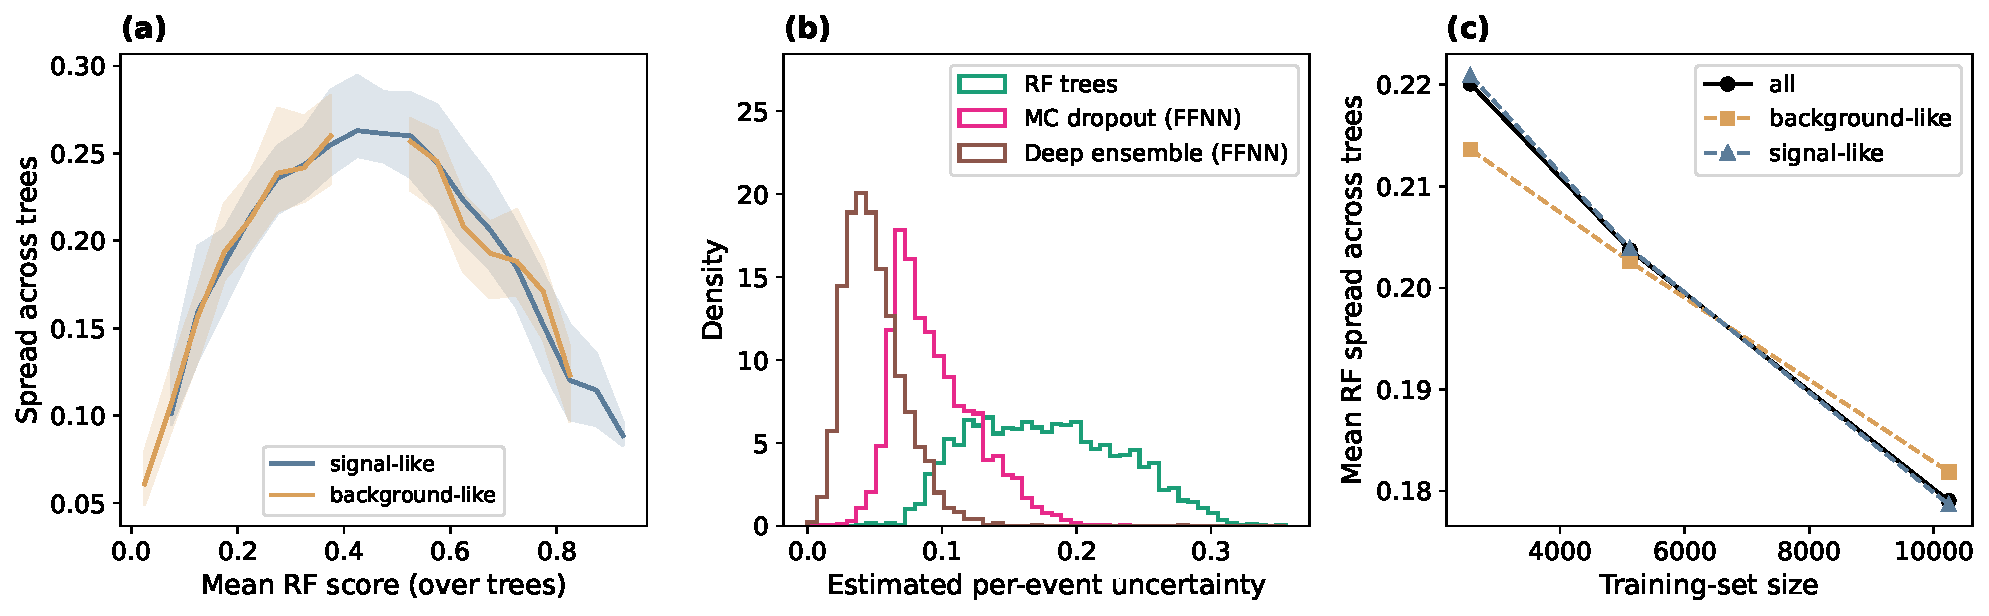
\includegraphics[width=0.95\textwidth]{figures/ml_nominal_uncertainty.pdf}
\caption{(a) Spread across the Random Forest trees vs.\ mean tree score, median and 16--84\% band of the test candidates of each weak-label class. (b) Distributions of the per-candidate uncertainty from the Random Forest trees, MC dropout and the deep ensemble. (c) Mean Random Forest spread vs.\ training-set size, for all, background-like and signal-like test candidates.}
\label{fig:ml_uncertainty}
\end{figure*}

The three estimators answer different questions, which explains the factor $\sim$3.5 between them. The deep ensemble only varies the initialization, on the same training data; MC dropout also perturbs the network structure; the trees of the Random Forest differ in their training data (bootstrap) and in the features they use, and each tree, of limited depth, is individually a poor and discrete estimator of $p$. Their per-candidate values are correlated but not interchangeable (Spearman correlations $0.41$--$0.57$ between pairs). The Random Forest spread contains both components. It is largest for scores around $0.5$ (Fig.~\ref{fig:ml_uncertainty}a), where the classes overlap and the trees disagree most -- an aleatoric contribution; and it decreases with the size of the training set, from $0.220$ with a quarter of it to $0.204$ with half and $0.179$ with the full set, while the test AUC stays at $0.860$--$0.862$ -- the epistemic contribution, which more data reduces.
\subsection{K-means on the Dalitz Plot}
\label{sec:ml_kmeans}
\emph{In short: for $K=8$ two clusters deviate by more than $3\sigma$ ($\chi^2=46.4$ for $7$ degrees of freedom): a negative asymmetry at low $m^2_{\mathrm{lo}}$ and positive ones at high $m^2_{\mathrm{hi}}$, as in the fixed binning.}
$K$-means is the unsupervised part of this analysis: it uses no labels, and the partition of the Dalitz plane is learned from the density of the candidates rather than fixed by hand. As an adaptive alternative to the fixed Dalitz-plot binning of Sec.~\ref{sec:bayes_dalitz}, the candidates of the fit window were partitioned with $K$-means~\cite{lloyd_kmeans} on the two standardized Dalitz variables $(m^2_{\mathrm{lo}},m^2_{\mathrm{hi}})$. $K$-means partitions the points $x_i$ into $K$ clusters $C_k$ minimizing the within-cluster sum of squares (inertia) $W=\sum_k\sum_{i\in C_k}\lVert x_i-\bar x_k\rVert^2$, with $\bar x_k$ the cluster centroids; $K$ has to be fixed in advance.
The quality of a partition is measured by the silhouette~\cite{silhouette}: for each point, $s_i=(b_i-a_i)/\max(a_i,b_i)$ compares its mean distance $a_i$ to the other points of its cluster with the mean distance $b_i$ to the points of the nearest other cluster, and the average over all points ($-1\le s\le 1$, higher is better) measures how well separated the clusters are. $K=8$ was fixed in advance, as a compromise between resolution and the number of candidates per cluster (at least $1233$), and $K=3$, the silhouette optimum over $K=2$--$12$ ($0.46$, against $0.41$ for $K=8$, a local maximum), was added. Both partitions are stable: repeating the clustering with a different random initialization gives an adjusted Rand index~\cite{hubert_ari} above $0.998$. Figure~\ref{fig:ml_kmeans_sel} shows the inertia and the silhouette against $K$: the inertia decreases monotonically and has no marked elbow, the silhouette has a global maximum at $K=3$ and a local one at $K=8$.

\begin{figure*}[t]
\centering
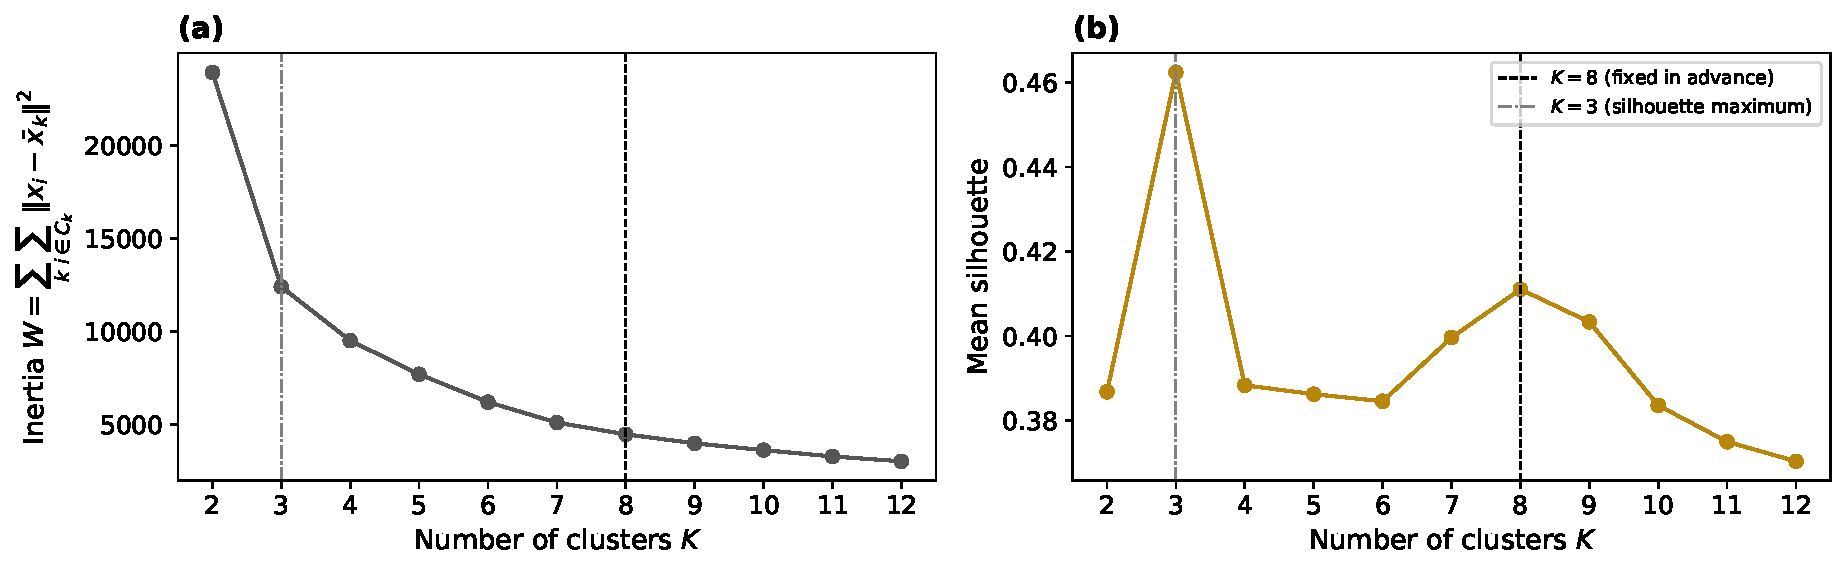
\includegraphics[width=0.85\textwidth]{figures/ml_kmeans_selection.pdf}
\caption{(a) Inertia and (b) mean silhouette of the $K$-means partition of the Dalitz plane for $K=2$--$12$; the dashed line marks the $K=8$ fixed in advance and the dash-dotted line the maximum of the silhouette, $K=3$.}
\label{fig:ml_kmeans_sel}
\end{figure*}

The asymmetry of each cluster was compared with the global one as in Sec.~\ref{sec:bayes_dalitz}, $S_k=(A_k-A_{\mathrm{glob}})/\sigma(A_k)$. For $K=8$ (Fig.~\ref{fig:ml_kmeans}), two clusters deviate by more than $3\sigma$ (probability $2\times10^{-4}$ for two or more if the asymmetry were uniform), and the homogeneity test gives $\chi^2=46.4/7$ ($p=7\times10^{-8}$). The most significant one lies at low $m^2_{\mathrm{lo}}$ ($1$--$2.5\,\GeV^2$) and intermediate $m^2_{\mathrm{hi}}$, with $A_k=-0.127\pm0.017$ ($n=3601$, $S_k=-5.1$); two clusters at high $m^2_{\mathrm{hi}}$ have positive asymmetries, $A_k=+0.020\pm0.020$ ($S_k=+3.2$) and $+0.040\pm0.028$ ($+2.9$). In the signal window ($|m-\mu|<2\sigma$) the same pattern is sharper -- three clusters beyond $3\sigma$, with $S_k=-5.6$, $+4.4$ and $+3.0$, and $\chi^2=62.3/7$ -- so it is not produced by the background. The coarser $K=3$ partition gives $\chi^2=15.2/2$ ($p=5\times10^{-4}$). The adaptive partition therefore confirms the picture of the fixed binning, a negative local asymmetry at low $m^2_{\mathrm{lo}}$ and positive ones at high $m^2_{\mathrm{hi}}$, with the same caveats (no background subtraction, no correction for detection asymmetries).

\begin{figure}[h]
\centering
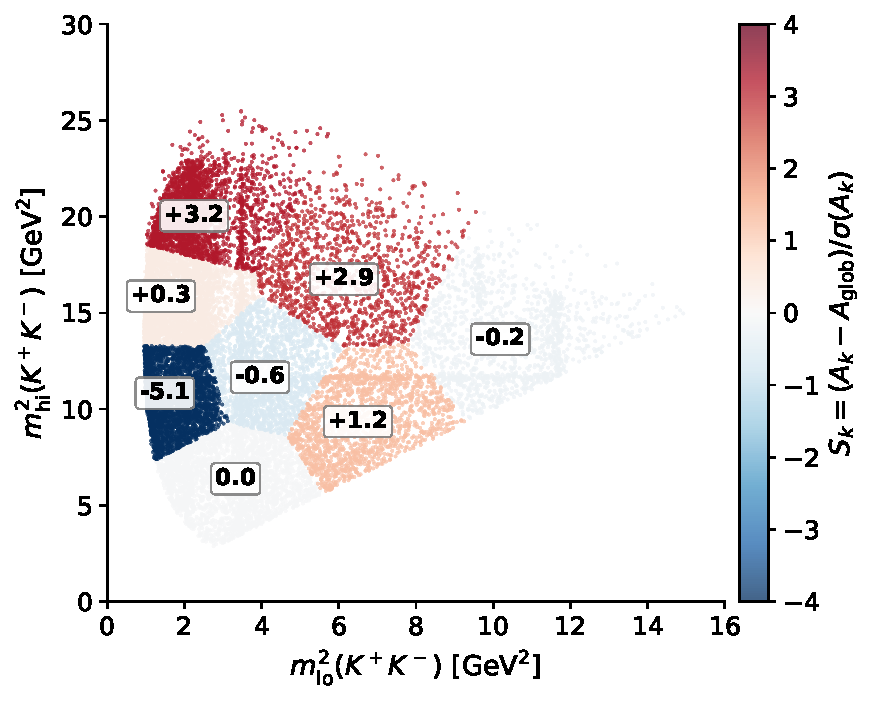
\includegraphics[width=\columnwidth]{figures/short_ml_kmeans.pdf}
\caption{$K$-means partition ($K=8$) of the Dalitz plane, all candidates of the fit window, same axes as Fig.~\ref{fig:bayes_dalitz}. Color and labels: local significance of each cluster with respect to the global asymmetry, $S_k=(A_k-A_{\mathrm{glob}})/\sigma(A_k)$, on the same scale as panel (c) of Fig.~\ref{fig:bayes_dalitz}.}
\label{fig:ml_kmeans}
\end{figure}

\subsection{Stability of $\Araw$ under ML Selection}
\label{sec:ml_stability}
\emph{In short: a cut on the score at $0.5$ keeps $92\%$ of the signal and $36\%$ of the background and leaves $\Araw$ within its expected statistical spread with both fits and with counting; it does not improve the precision and cannot remove the misidentified background.}

The reference (gradient-boosting) score was applied to all candidates of the fit window (on the test set, a cut at $0.5$ keeps $88\%$ of the signal-like and $28\%$ of the background-like candidates, Fig.~\ref{fig:ml_roc}), not only to the labeled ones used in training, and the counting asymmetry was recomputed after cuts on the score from $0.1$ to $0.9$ (Fig.~\ref{fig:ml_threshold}). Since every selected sample is contained in the full one, the expected statistical spread of the difference is $\sqrt{\sigma_{\mathrm{sub}}^2-\sigma_{\mathrm{full}}^2}$, not the uncertainty of either estimate. Over all thresholds, which keep from $18{,}443$ to $2621$ candidates, the shift with respect to the full window ($A_{\mathrm{count}}=-0.0432$) stays within $1.4$ times this spread: the selection does not introduce a detectable bias in the counting asymmetry. Split by magnet polarity at a cut of $0.5$, the counting asymmetries are $-0.060\pm0.010$ (down) and $-0.024\pm0.012$ (up), $2.2\sigma$ apart; the Frequentist fit of the same samples, which separates the background, gives $-0.054\pm0.011$ and $-0.032\pm0.013$, $1.3\sigma$ apart (against $0.7\sigma$ for the full sample, Sec.~\ref{sec:bayes_checks}), so most of the larger difference of the counting estimates comes from the background.

\begin{figure}[h]
\centering
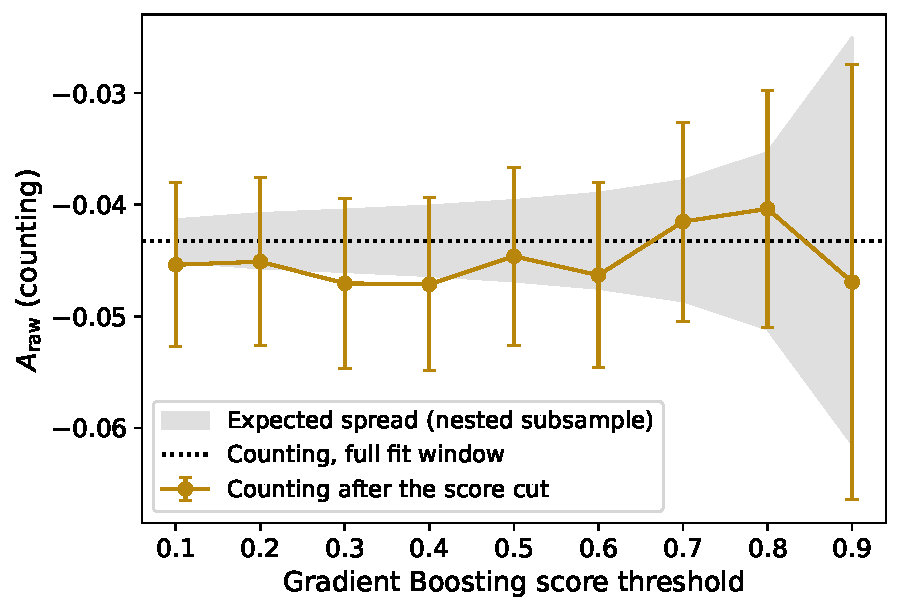
\includegraphics[width=\columnwidth]{figures/ml_nominal_threshold.pdf}
\caption{Counting asymmetry after a cut on the gradient-boosting score, vs.\ threshold, with its binomial uncertainty. Dotted line: counting asymmetry of the full fit window; band: expected statistical spread of a nested subsample around it, $\pm\sqrt{\sigma_{\mathrm{sub}}^2-\sigma_{\mathrm{full}}^2}$.}
\label{fig:ml_threshold}
\end{figure}

Counting cannot reveal whether the selection deforms the mass spectrum. To test this, the selected sample (score $>0.5$, $15{,}709$ candidates) was refitted with the nominal mass model by both inference methods of this work, the Bayesian fit of Sec.~\ref{sec:bayesian} and the Frequentist maximum-likelihood fit of Sec.~\ref{sec:frequentist}, and the three estimates were compared with those of the full sample (Table~\ref{tab:three_methods}, Fig.~\ref{fig:ml_three}). The asymmetry is stable: all three shifts are within their expected nested-sample spread, and the significance of $A\neq0$ from the profile likelihood (Wilks' theorem~\cite{wilks}) is $5.2\sigma$ in both samples. The same holds for the tighter cut at the maximum of the significance improvement (score $>0.73$, $\varepsilon_S=0.66$, $\varepsilon_B=0.13$, Fig.~\ref{fig:ml_roc}b): the three shifts, $+0.004$ to $+0.005$, are $0.9$ times their expected spread, and $A\neq0$ is still $4.1\sigma$. This cut is not an optimum for the measurement: the figure of merit $\varepsilon_S/\sqrt{\varepsilon_B}$ holds for a signal small against the background, while here the precision follows $S/\sqrt{S+B}$ and worsens from $0.0085$ to $0.0097$. The selection keeps $92\%$ of the fitted signal and $36\%$ of the background ($N_s=14{,}121$, $N_b=1590$), but this does not improve the precision on $\Araw$ ($0.0087$ against $0.0085$): the background under the peak is already small ($\approx$4\% in the signal window) and the fit separates it from the signal anyway.

\begin{table*}[t]
\centering
\begin{tabular}{lccccc}
\toprule
Method & Full sample & Score $>0.5$ & Shift (expected) & Score $>0.73$ & Shift (expected) \\
\midrule
Bayesian fit    & $-0.0443\pm0.0085$ & $-0.0451\pm0.0087$ & $-0.0008\,(0.0018)$ & $-0.0404\pm0.0097$ & $+0.0039\,(0.0047)$ \\
Frequentist fit & $-0.0441\pm0.0085$ & $-0.0447\pm0.0086$ & $-0.0006\,(0.0012)$ & $-0.0401\pm0.0097$ & $+0.0040\,(0.0048)$ \\
Counting        & $-0.0432\pm0.0071$ & $-0.0446\pm0.0080$ & $-0.0014\,(0.0036)$ & $-0.0381\pm0.0093$ & $+0.0051\,(0.0059)$ \\
\bottomrule
\end{tabular}
\caption{$\Araw$ on the full fit window ($19{,}731$ candidates) and after the cuts on the gradient-boosting score at $0.5$ ($15{,}709$ candidates) and at $0.73$ ($11{,}658$), the maximum of the significance improvement of Fig.~\ref{fig:ml_roc}, by the three methods. The expected shift is the statistical spread of a nested subsample, $\sqrt{\sigma_{\mathrm{sub}}^2-\sigma_{\mathrm{full}}^2}$. Counting includes the background.}
\label{tab:three_methods}
\end{table*}

\begin{figure}[h]
\centering
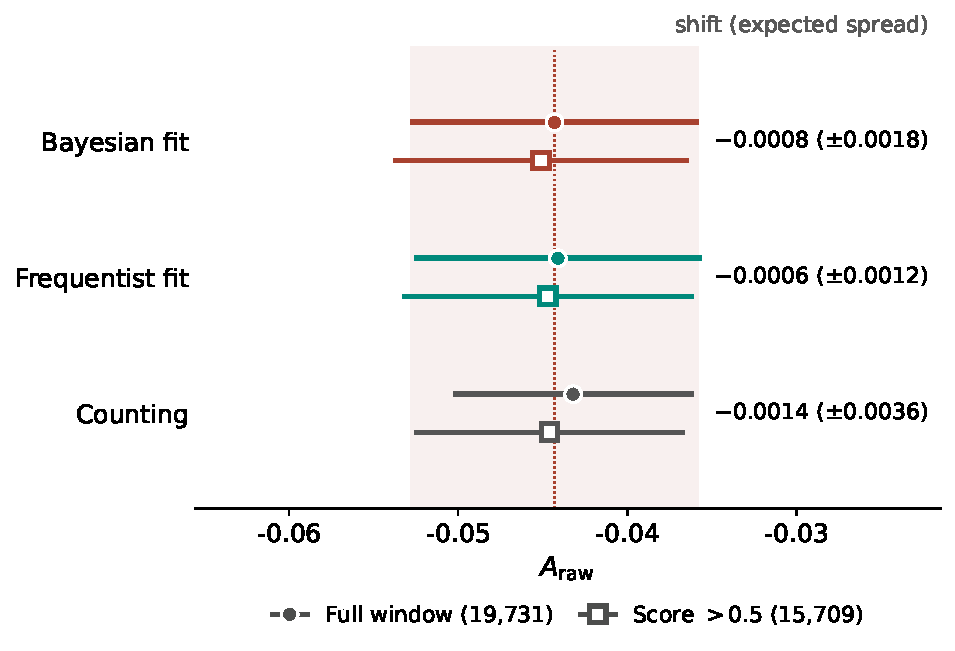
\includegraphics[width=\columnwidth]{figures/short_ml_three.pdf}
\caption{$\Araw$ from the Bayesian fit, the Frequentist fit and counting, for the full sample and the ML-selected ones, at a score cut of $0.5$ and at $0.73$, the maximum of the significance improvement (Table~\ref{tab:three_methods}).}
\label{fig:ml_three}
\end{figure}

The mass spectrum, instead, changes. The goodness of fit of the nominal model degrades from $\chi^2=164/88$ to $253/88$ in the Bayesian fit and from $442/388$ to $557/388$ in the Frequentist one (with a different binning), and the background shape changes: the slope of the slow exponential grows from $0.0028$ to $0.0071\,\MeV^{-1}$ ($B^+$) and from $0.0016$ to $0.0057\,\MeV^{-1}$ ($B^-$), and the fraction of the steep one from $0.11$ to $0.28$ and from $0.21$ to $0.50$.
Two mechanisms can produce this: the classifier could reconstruct the mass from the kaon momenta and sculpt the background (Sec.~\ref{sec:ml_labels}), or the selection could change the composition of the background. The first is excluded: the same classifier trained without the nine momentum components (test AUC $0.860$) gives the same degradation ($\chi^2=533/388$).
The efficiency of the cut as a function of the mass shows the second (Fig.~\ref{fig:ml_mass_cut}): it is $0.89$--$0.90$ at the peak, $\approx0.70$ below $5150\,\MeV$ and $0.06$--$0.13$ above $5375\,\MeV$. The classifier does what it is trained for -- it removes the combinatorial background and keeps genuine $B$ decays, including the partially reconstructed ones and the other non-combinatorial components that the weak labels cannot separate from the signal. In the selected sample these components weigh relatively more, and the nominal model, which has no dedicated component for them, describes it worse, mostly under the peak (the $\chi^2$ of the $\pm4\sigma$ region grows from $75$ to $134$ for 30 bins) and below it. A Crystal Ball signal gives the same degradation ($407\to522$ for 386 degrees of freedom), so it is not due to the signal tails.

\begin{figure*}[t]
\centering
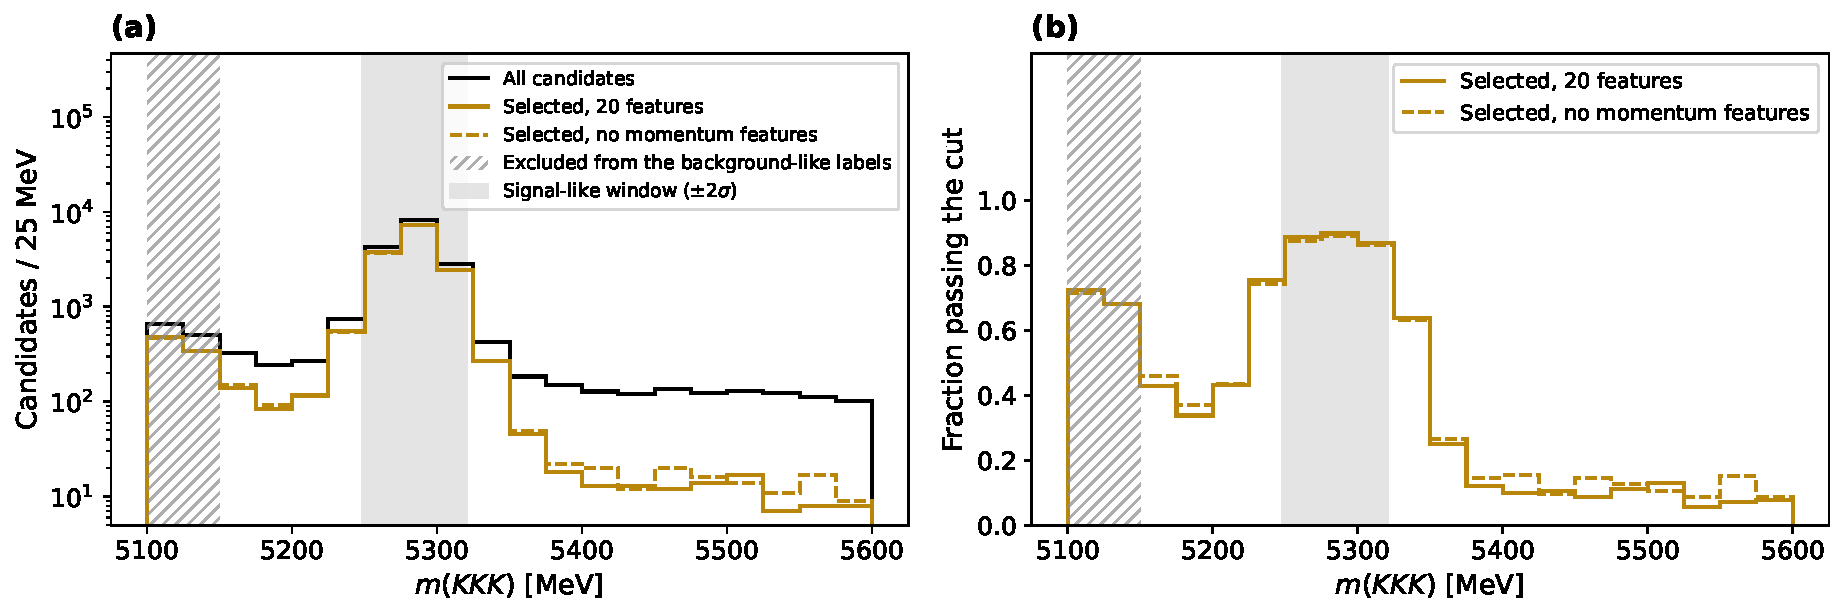
\includegraphics[width=0.95\textwidth]{figures/ml_nominal_mass_after_cut.pdf}
\caption{(a) Mass spectrum of all candidates and of those with gradient-boosting score $>0.5$, for the 20-feature classifier and for one trained without the kaon momentum components (25\,MeV bins). (b) Fraction of candidates passing the cut. Hatched: the region below $5150\,\MeV$ excluded from the background-like labels; grey: the signal-like window.}
\label{fig:ml_mass_cut}
\end{figure*}

$\Araw$ is unaffected because it is determined by the peak and the background shape is free in the fit, but a measurement that relied on the background shape, or on a background model taken from the sidebands of the full sample, would be biased by the selection.

In the nominal sample the selection cannot improve the precision because there is little background to remove. To test it where the background is larger, the same study was repeated on a sample with a looser kaon identification, $\texttt{ProbK}>0.3$ ($33{,}328$ candidates, signal purity $94\%$ within $\pm2\sigma$ of the peak), with the reference classifier retrained on the weak labels of this sample (test AUC $0.895$). Cleaning it with a cut on the classifier score is compared with tightening the identification cut, at equal signal efficiency (Fig.~\ref{fig:ml_high_bkg}). The classifier removes the combinatorial background with little signal loss -- a cut at $0.5$ keeps $93\%$ of the signal and raises the purity to $99\%$ -- and at any efficiency gives a slightly smaller $\sigma(\Araw)$ than the identification cut. The gain is small ($0.0072\to0.0070$ at best): loosening the identification adds mostly signal ($+47\%$ with respect to the nominal selection), and the background under the peak stays a small fraction.

\begin{figure*}[t]
\centering
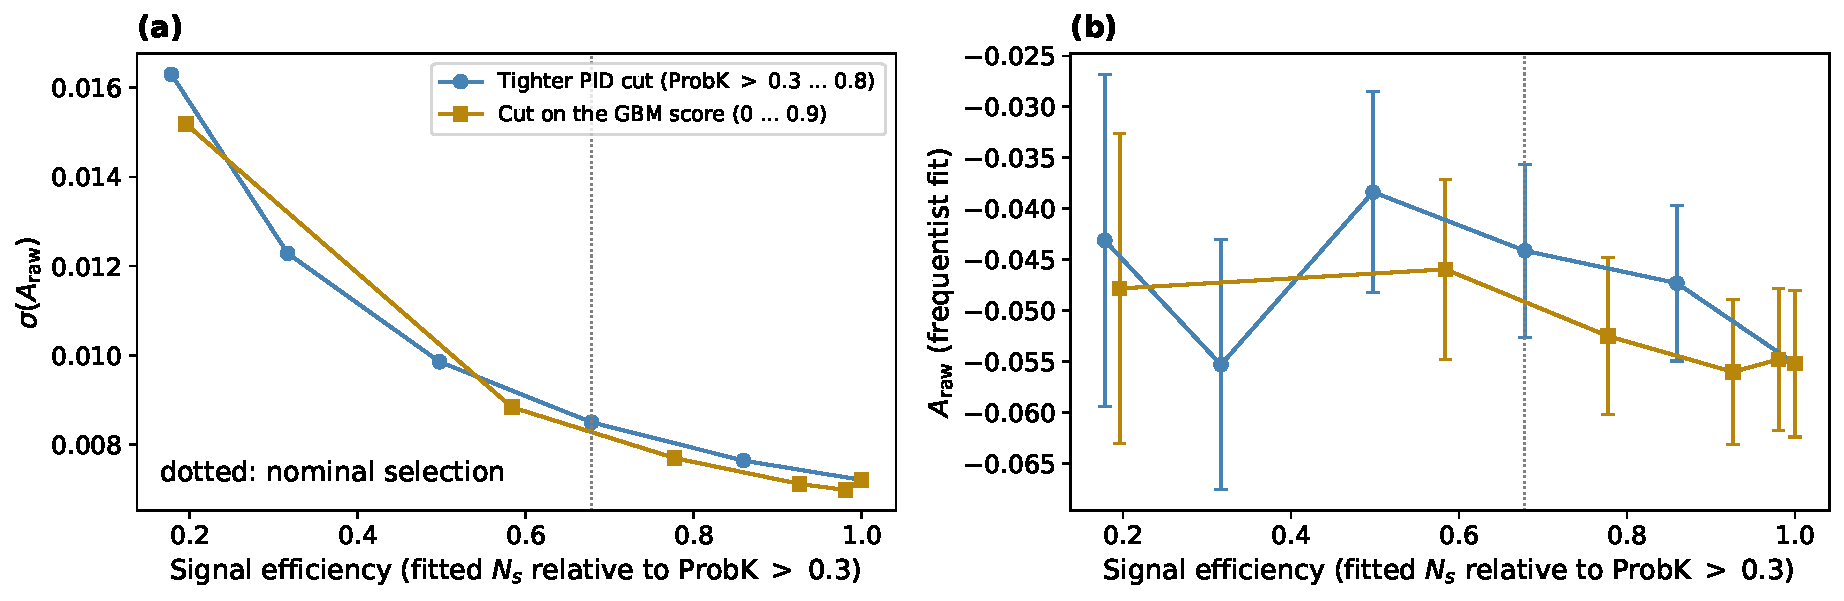
\includegraphics[width=0.95\textwidth]{figures/ml_nominal_high_background.pdf}
\caption{High-background sample ($\texttt{ProbK}>0.3$): (a) statistical uncertainty and (b) value of $\Araw$ from the Frequentist fit vs signal efficiency, for tighter identification cuts ($\texttt{ProbK}>0.3,\dots,0.8$) and for cuts on the score of the classifier retrained on this sample ($0,\dots,0.9$). The dotted line marks the nominal selection ($\texttt{ProbK}>0.5$). The samples are nested, so their uncertainties are correlated.}
\label{fig:ml_high_bkg}
\end{figure*}

The classifier also cannot remove the background that matters for $\Araw$. With the looser identification the asymmetry moves to $-0.055$, as expected from misidentified $B^\pm\to\pi^\pm K^+K^-$ decays (Sec.~\ref{sec:syst}); tightening the identification cut to $\texttt{ProbK}>0.4$ moves it back by $+0.008$ ($3.3$ times the nested-sample spread), while the score cut that keeps $93\%$ of the signal moves it by $-0.001$. Misidentified $B$ decays peak close to the $B$ mass, so the mass-based weak labels mark them as signal-like: the CWoLa classifier, by construction, cannot learn to reject a background that sits under the peak, and particle identification remains necessary.
\subsection{Hyperparameter Optimization}
\label{sec:ml_hyper}
\emph{In short: the best configurations improve the test AUC by at most $0.005$, less than its uncertainty, and the cross-validated maximum overestimates the test AUC (winner's curse).}
The hyperparameters of the Random Forest ($120$ configurations), gradient boosting ($100$) and the FFNN ($168$: seven architectures, four dropout rates, six learning rates) were optimized by repeated cross-validation on the training set (Tables~\ref{tab:ml_hyperparams}--\ref{tab:ml_ffnn_search}). The best configurations improve the test AUC over the defaults of Table~\ref{tab:ml_models} by $0.005$ (Random Forest), $0.001$ (gradient boosting) and $0.004$ (FFNN), all well below the test-set uncertainty ($0.012$) and, for the FFNN, comparable with its spread over initializations ($0.005$). For the two tree ensembles the best cross-validated AUC is higher than the test AUC of the same configuration ($0.871$ vs $0.866$ and $0.868$ vs $0.865$), as expected when the maximum is taken over many noisy cross-validation estimates (the ``winner's curse''): the selection favors configurations with a favorable fluctuation, and the cross-validated score of the selected configuration is an optimistic estimate of its performance. Figure~\ref{fig:ml_ffnn_search} shows the cross-validated AUC of the $168$ network configurations by architecture: the best value rises from $0.839$ (one layer of $8$ units) to $0.858$ (two or three layers) and then saturates ($0.857$ and $0.854$ for four and five layers), while the spread within each architecture is dominated by the learning rate and the dropout. The searches show that the defaults are already close to optimal for this problem, so the defaults are used throughout.

\begin{figure}[h]
\centering
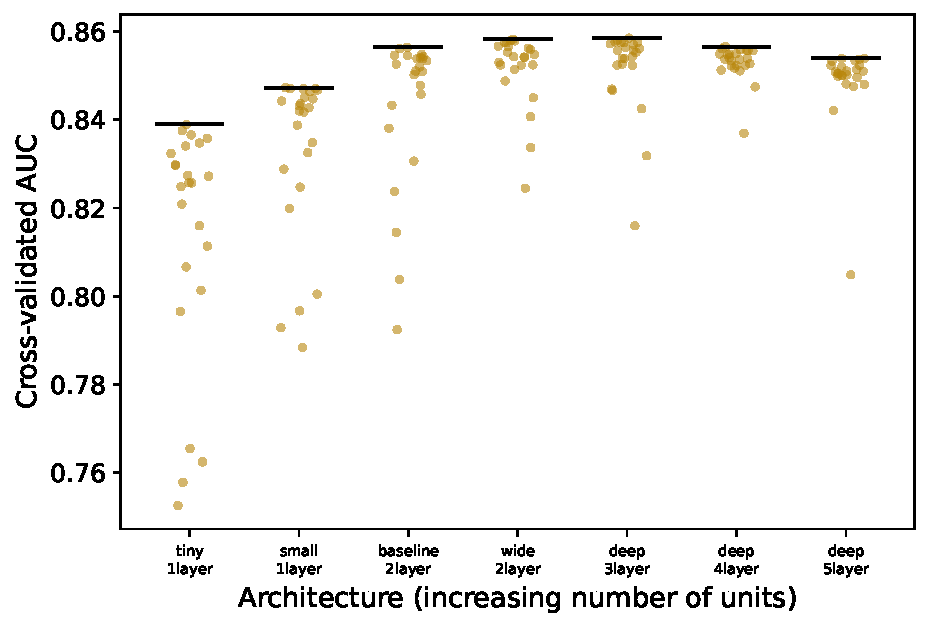
\includegraphics[width=\columnwidth]{figures/ml_ffnn_search.pdf}
\caption{Cross-validated AUC of the $168$ FFNN configurations (dots) for each of the seven architectures, ordered by number of units; the black segment marks the best configuration of each architecture.}
\label{fig:ml_ffnn_search}
\end{figure}

\begin{table*}[t]
\centering
\begin{tabular}{lllc}
\toprule
Model & \pcell{7cm}{Grid} & Best configuration & CV AUC / Test AUC (default) \\
\midrule
Random Forest & \pcell{7cm}{\texttt{n\_estimators} $200$--$1200$, \texttt{max\_depth} $6$--$12$ or none, \texttt{min\_samples\_leaf} $5$--$40$} & $400$, $12$, $5$ & $0.8706$ / $0.8656$ ($0.8604$) \\
Gradient Boosting & \pcell{7cm}{\texttt{n\_estimators} $100$--$500$, \texttt{max\_depth} $1$--$5$, \texttt{learning\_rate} $0.01$--$0.1$} & $300$, $2$, $0.1$ & $0.8684$ / $0.8650$ ($0.8643$) \\
\bottomrule
\end{tabular}
\caption{Hyperparameter search for the tree ensembles ($120$ and $100$ configurations, 5-fold cross-validation repeated 10 times, balanced class weights). The test AUC of the best configuration is compared with that of the default of Table~\ref{tab:ml_models} (in parentheses); the bootstrap uncertainty of each test AUC is $0.012$.}
\label{tab:ml_hyperparams}
\end{table*}

\begin{table*}[t]
\centering
\begin{tabular}{llccc}
\toprule
Architecture & Layers & Dropout & Learning rate & CV AUC \\
\midrule
\texttt{deep\_3layer} (best) & $[64,32,16]$ & $0.2$ & $0.003$ & $0.8585\pm0.0174$ \\
\texttt{wide\_2layer}        & $[64,32]$    & $0.3$ & $0.003$ & $0.8582\pm0.0175$ \\
\texttt{deep\_3layer}        & $[64,32,16]$ & $0.3$ & $0.003$ & $0.8580\pm0.0187$ \\
\texttt{wide\_2layer}        & $[64,32]$    & $0.3$ & $0.005$ & $0.8579\pm0.0184$ \\
\texttt{wide\_2layer}        & $[64,32]$    & $0.4$ & $0.005$ & $0.8579\pm0.0187$ \\
\bottomrule
\end{tabular}
\caption{Top five of the $168$ FFNN configurations ($7$ architectures from one hidden layer of 8 units to five layers $[128,64,32,16,8]$, dropout $0.1$--$0.4$, learning rates $0.0002$--$0.005$; 5-fold cross-validation repeated twice). The five are within $0.0007$ of each other, far below the fold-to-fold spread: the optimum is a plateau. The best configuration has test AUC $0.8606$, against $0.8568$ for the default architecture ($\pm0.005$ over initializations).}
\label{tab:ml_ffnn_search}
\end{table*}

\subsection{Local Asymmetries: Fixed Binning and $K$-Means}
\label{sec:comparison_local}
\emph{In short: the fixed grid and the $K$-means partition show the same pattern, a negative asymmetry at low $m^2_{\mathrm{lo}}$ and positive ones at high $m^2_{\mathrm{hi}}$ ($\chi^2=80.8/31$ and $46.4/7$).}
Two partitions of the Dalitz plane were used, a fixed $8\times8$ grid (Sec.~\ref{sec:dalitz}) and an adaptive $K$-means partition with $K=8$ (Sec.~\ref{sec:ml_kmeans}). Both find that the asymmetry is not uniform: $\chi^2=80.8$ for $31$ degrees of freedom for the grid and $46.4$ for $7$ for $K$-means ($p=3\times10^{-6}$ and $7\times10^{-8}$). Both place the negative local asymmetry at low $m^2_{\mathrm{lo}}$ and intermediate $m^2_{\mathrm{hi}}$ ($A=-0.128\pm0.018$ in the region of the two significant bins, $-0.127\pm0.017$ in the most significant cluster) and positive deviations at high $m^2_{\mathrm{hi}}$. The two partitions have different bins, so the numbers are not independent, and the $K$-means $p$-value benefits from the larger bins; the agreement is in the pattern. In the region defined by the published analysis, fixed before looking at the data, both fits give a compatible value ($-0.234\pm0.025$ Bayesian, $-0.237\pm0.025$ Frequentist, $9.4\sigma$ from zero) with $-0.239\pm0.020$. All local numbers are counting asymmetries or fits of the integrated mass spectrum in a region, with no background subtraction by event weights and no correction for detection asymmetries (Sec.~\ref{sec:limitations}).
\FloatBarrier

\section{Comparison and Discussion}
\label{sec:comparison}
\label{app:ext_comp}
\emph{In short: the Frequentist and Bayesian analyses give the same value, uncertainty and coverage for $\Araw$ because they use the same likelihood and the data constrain it well; they differ in what the numbers mean and in the hypothesis tests, and a machine-learning selection (Sec.~\ref{sec:ml}) confirms the result without improving it.}
\label{sec:comparison_summary}
The Frequentist and Bayesian analyses agree on every number and differ in what each number means. Table~\ref{tab:comparison} puts the two approaches side by side, from the question each one asks to how it was validated; the subsections explain the rows where the numbers coincide but the statements do not.

\begin{table*}[t]
\centering
\small
\begin{tabular}{lll}
\toprule
 & \pcell{6.6cm}{Frequentist (Sec.~\ref{sec:frequentist})} & \pcell{6.6cm}{Bayesian (Sec.~\ref{sec:bayesian})} \\
\midrule
\pcell{2.6cm}{Question} & \pcell{6.6cm}{Which value of $A$ makes the data most probable, and which values are not rejected?} & \pcell{6.6cm}{What is the distribution of $A$ given the data and the prior?} \\
\pcell{2.6cm}{Estimate} & \pcell{6.6cm}{Maximum likelihood, $-0.0441$} & \pcell{6.6cm}{Posterior median, $-0.0443$ (mode $-0.0441$)} \\
\pcell{2.6cm}{Interval (68\%)} & \pcell{6.6cm}{$[-0.0526,-0.0356]$ (profile likelihood, Minos)} & \pcell{6.6cm}{$[-0.0528,-0.0358]$ (credible, equal-tailed)} \\
\pcell{2.6cm}{Nuisance parameters (11)} & \pcell{6.6cm}{profiled: re-minimized at each fixed $A$} & \pcell{6.6cm}{marginalized: integrated over the prior} \\
\pcell{2.6cm}{Test of $A=0$} & \pcell{6.6cm}{$q(0)\simeq27$, $p=2.05\times10^{-7}$, $5.2\sigma$} & \pcell{6.6cm}{$BF_{01}\approx1.1\times10^{-4}$ (Savage-Dickey)} \\
\pcell{2.6cm}{Validation of the interval} & \pcell{6.6cm}{$1000$ bootstrap replicas: $68.4\pm1.5\%$; $985$ toys: $70\pm1\%$ ($68\%$), $95\pm1\%$ ($95\%$)} & \pcell{6.6cm}{$200$ toys: $0.65\pm0.03$ ($68\%$), $0.93\pm0.02$ ($95\%$)} \\
\pcell{2.6cm}{Goodness of fit} & \pcell{6.6cm}{$\chi^2/\mathrm{ndof}\approx160/88$ ($10\,\MeV$ bins); $441.7/388$, $p=0.031$ ($2.5\,\MeV$ bins)} & \pcell{6.6cm}{$164.1/88$ ($p=1.6\times10^{-6}$); posterior predictive check} \\
\pcell{2.6cm}{Computing time} & \pcell{6.6cm}{one joint fit with Minos $\simeq19\,$s; $1000$ bootstrap fits $\simeq49\,$min} & \pcell{6.6cm}{one chain ($25{,}000$ steps, 32 walkers) $\simeq8\,$min; $200$ toys of $12{,}000$ steps} \\
\bottomrule
\end{tabular}
\caption{Frequentist and Bayesian analyses compared on the same candidates ($\Araw$, statistical uncertainties only). Computing times are indicative, on one laptop.}
\label{tab:comparison}
\end{table*}

\subsection{Where the Approaches Differ}
\label{sec:comparison_differ}
\emph{In short: the numbers coincide but the statements differ: the meaning of the interval, the test of $A=0$, the goodness of fit, the treatment of the nuisance parameters and what has been validated, as summarized in Table~\ref{tab:comparison}.}
\emph{Meaning of the interval.} The credible interval states that, given the data and the prior, $A$ lies in $[-0.0528,-0.0358]$ with $68\%$ probability; the confidence interval $[-0.0526,-0.0356]$ is the set of values that the data do not reject at the $32\%$ level, and the $68\%$ is the fraction of repeated experiments in which such an interval contains the true value, a property of the procedure that the bootstrap and toy checks verified. Figure~\ref{fig:checks_profile} shows the two for $A$: the profile likelihood and the marginal posterior coincide (a), and the profile curves of the two magnet polarities add up to that of the joint fit (b).

\begin{figure*}[t]
\centering
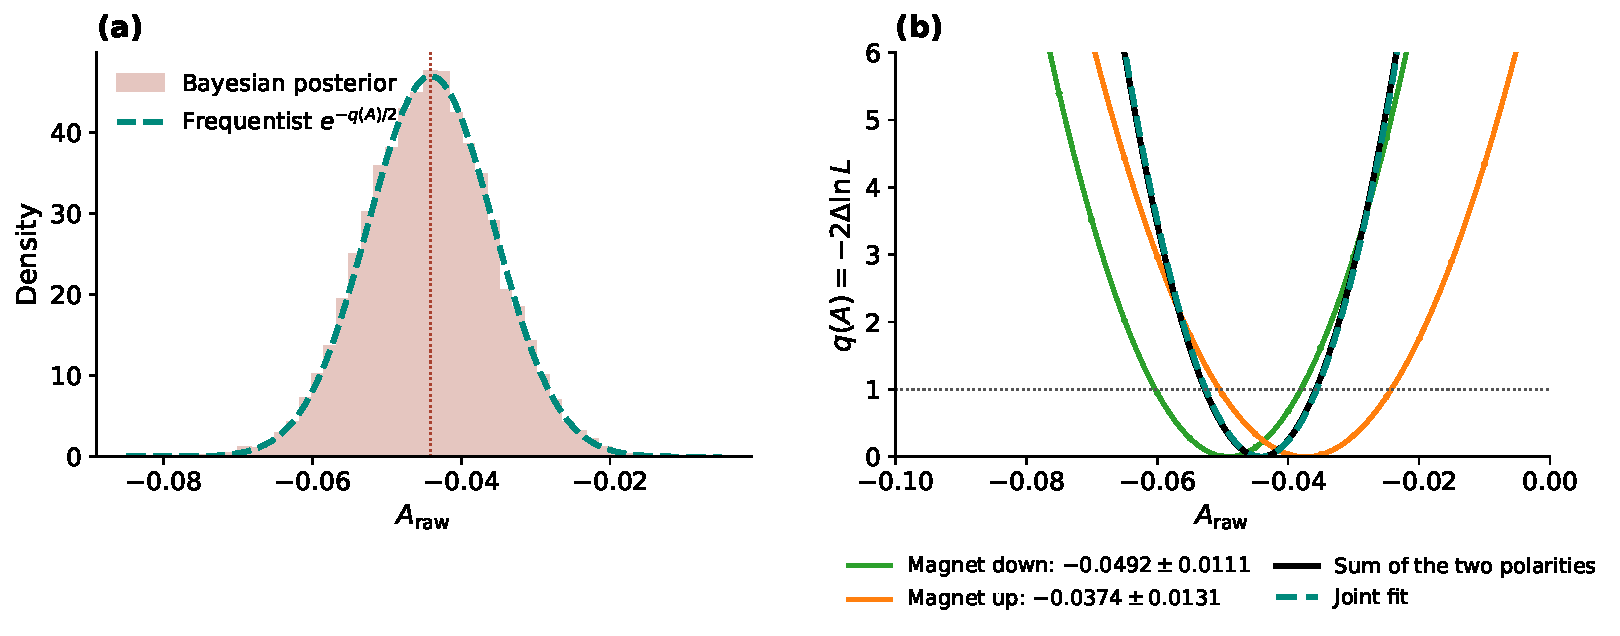
\includegraphics[width=0.95\textwidth]{figures/short_profile_polarity.pdf}
\caption{(a) Frequentist profile likelihood, $\exp[-q(A)/2]$ normalized, and Bayesian marginal posterior of $A$. (b) Profile curves $q(A)$ of the two magnet polarities (parabolic fits to the points), their sum and the joint fit.}
\label{fig:checks_profile}
\end{figure*}

\emph{Hypothesis test.} Three tests of $A=0$ are available. The exact binomial test of $N^-=N^+$ on all candidates gives $6.1\sigma$ ($A_{\mathrm{count}}=-0.0432\pm0.0071$); it sees signal and background together and does not use the mass. The Frequentist test of the fit gives $p=2\times10^{-7}$ ($Z=\sqrt{q(0)}=5.2\sigma$ in the two-sided convention, $5.06\sigma$ one-sided, Sec.~\ref{sec:appendix_freq}), independent of the prior and not the probability of $A=0$; its size and power were verified with toy MC (Sec.~\ref{sec:validation_power}).
The Bayes factor, $BF_{10}\approx9\times10^3$, depends on the prior width (Sec.~\ref{sec:bayes_factor}). For $A$ the Frequentist and Bayesian tests give the same conclusion; for the background asymmetry, $A_b=-0.040\pm0.018$, a Frequentist test would call $2.3\sigma$ a hint while $BF_{01}\approx3.5$ mildly favors $A_b=0$: the $p$-value asks how improbable the data are under $A_b=0$, the Bayes factor which hypothesis the data prefer after the prior volume is accounted for.
\subsection{Comparison with the Published Analysis}
\label{sec:comparison_published}
\emph{In short: the published value ($-0.060\pm0.007$) differs from this one ($-0.0441\pm0.0085$) by the sample and the model; with the same $D^0$ veto the Bayesian fit gives $-0.0496\pm0.0088$, and $\Araw$ is not $\ACP$.}
The published analysis~\cite{lhcb_cpv_2013} finds $\Araw=-0.060\pm0.007$ with $22{,}119\pm164$ signal candidates, against $-0.0441\pm0.0085$ and $15{,}328\pm133$ here: the Open Data record is a preselected subset and the published model has a Cruijff signal, partially reconstructed four-body decays and a misidentified peaking background from simulation. With the same $D^0$ veto the Bayesian fit gives $-0.0496\pm0.0088$, within $0.93\sigma$ of the published value.
The raw asymmetry is not the CP asymmetry: $\ACP\approx\Araw-A_P-A_D$ (Eq.~\eqref{eq:acp}), and in the published analysis the corrections move the result from $-0.060$ to $-0.043\pm0.009\pm0.003\pm0.007$ ($3.7\sigma$)~\cite{lhcb_cpv_2013}, by $+0.017$, about two statistical uncertainties of this work. Such a correction cannot be assumed for a different selection, and the $5.2\sigma$ here is the significance of a nonzero raw asymmetry, not of CP violation. A later measurement on a larger data set gives $\ACP=-0.037\pm0.002\pm0.002\pm0.003$ ($8.5\sigma$)~\cite{lhcb_cpv_prd2023,lhcb_cpv_paper}; our result is consistent with these in sign and size.
\subsection{Machine-Learning Cross-Check}
\label{sec:comparison_mlcheck}
\emph{In short: a classifier trained on weak labels from the mass spectrum selects candidates without changing $\Araw$ beyond its statistical spread; it does not improve the precision and cannot remove the misidentified decays under the signal (Sec.~\ref{sec:ml}).}
A cut at $0.5$ on the classifier score keeps $92\%$ of the fitted signal and $36\%$ of the background and gives $\Araw=-0.0451\pm0.0087$ (Bayesian) and $-0.0447\pm0.0086$ (Frequentist), against $-0.0443$ and $-0.0441$ for the full window: both shifts are within the statistical spread expected for a subsample (Sec.~\ref{sec:ml_stability}, Fig.~\ref{fig:ml_three}). The precision does not improve because the nominal sample has little background to remove; the classifier is described in Sec.~\ref{sec:ml}.
\subsection{Numerical Agreement}
\label{sec:comparison_numbers}
\emph{In short: the two fits agree to the quoted digits (estimates differ by $0.0002$, both uncertainties are $0.0085$, systematic uncertainties $0.0070$ and $0.0072$); sideband subtraction gives $-0.0503\pm0.0083$.}
The two fits of the same model agree to the precision of the quoted digits: the estimates differ by $0.0002$ ($0.02$ standard deviations), the uncertainties are both $0.0085$, the $68\%$ and $95\%$ intervals differ by at most $0.0002$, and the shifts of the thirteen systematic variants agree within $0.0005$, with the same group uncertainties for the window ($0.0014$) and the preselection ($0.0058$) and slightly different ones for the background ($0.0037$ against $0.0040$) and the signal model ($0.0002$ against $0.0006$), so that the total systematic uncertainties are $0.0070$ and $0.0072$ (Sec.~\ref{sec:syst}). A third estimate, by sideband subtraction (counting in the signal region after removing the background expected from the sideband fit), gives $-0.0503\pm0.0083$, which differs from the nominal value by $0.006$, less than one standard deviation, on the same candidates. This is expected, and it is not by itself a validation of the model. With $\sim2\times10^4$ candidates and flat priors the posterior is proportional to the likelihood, the likelihood is close to a Gaussian in $A$, and the posterior mode coincides with the maximum-likelihood estimate; the posterior median, the posterior mean and the mode differ by less than $2\times10^{-4}$. What the agreement does show is that neither the sampling (MCMC) nor the asymptotic approximations (Hesse, Wilks) introduce a bias: the Bayesian intervals have the coverage of the Frequentist ones (Sec.~\ref{sec:bayes_toymc}) and the profile-likelihood interval has the coverage assumed by Wilks' theorem (Sec.~\ref{sec:freq_coverage}).
The agreement does not extend to the validity of the model itself. Both methods describe the same spectrum with the same Gaussian signal and double-exponential background, and neither reaches $\chi^2/\mathrm{ndof}\approx1$ (Sec.~\ref{sec:bayes_gof}); what protects $\Araw$ is that its value does not depend on the signal shape (shift $-0.0002$ with a Crystal Ball) and that the background treatment, the largest model dependence, is included in the systematic uncertainty.
\subsection{Profile Likelihood, Posterior and the Two Polarities}
\label{sec:checks_profile}
\emph{In short: profiling and marginalizing the nuisance parameters give the same distribution of $A$; the two magnet polarities agree with each other, and combining their likelihoods reproduces the joint fit.}
The Frequentist way of eliminating the nuisance parameters is to profile them, $q(A)=-2\Delta\ln L$ with the other parameters re-maximized at each $A$, the Bayesian one is to marginalize them; Fig.~\ref{fig:checks_profile}a shows that $\exp[-q(A)/2]$, normalized, and the marginal posterior coincide, as expected for a near-Gaussian likelihood and flat priors. The two polarities were fitted separately and their profile curves added, which is the combination of likelihoods of two independent measurements of the same parameter (Fig.~\ref{fig:checks_profile}b): magnet down gives $-0.0492\pm0.0111$, magnet up $-0.0374\pm0.0131$, their sum $-0.0443\pm0.0084$, against $-0.0441\pm0.0085$ of the joint fit (the nuisance parameters are shared in the joint fit, separate in the sum). The Bayesian counterpart is sequential: the posterior of magnet down used as the prior of magnet up gives $-0.0446\pm0.0086$ (Table~\ref{tab:checks_polarity}).

\begin{table}[h]
\centering
\resizebox{\ifdim\width>\linewidth\linewidth\else\width\fi}{!}{\begin{tabular}{lcc}
\toprule
 & Frequentist & Bayesian \\
\midrule
Magnet down & $-0.0492\pm0.0111$ & $-0.0497\pm0.0112$ \\
Magnet up & $-0.0374\pm0.0131$ & $-0.0378\pm0.0129$ \\
Combination of the two & $-0.0443\pm0.0084$ & $-0.0446\pm0.0086$ \\
Joint fit & $-0.0441\pm0.0085$ & $-0.0443\pm0.0085$ \\
\bottomrule
\end{tabular}}
\caption{$\Araw$ for the two magnet polarities and their combination, by the two methods; the Frequentist combination is the sum of the profile likelihoods of the two polarities, the Bayesian one the sequential update of the posterior.}
\label{tab:checks_polarity}
\end{table}

\subsection{Confidence and Credible Regions in $(A,A_b)$}
\label{sec:checks_region}
\emph{In short: the $68\%$ and $95\%$ regions of the Frequentist profile ($\Delta\mathrm{NLL}$ at the $\chi^2_2$ values $2.30$ and $5.99$) and of the Bayesian highest posterior density coincide, and $A=0$ lies outside both.}
For two parameters of interest the Wilks statistic follows a $\chi^2$ with two degrees of freedom (Fig.~\ref{fig:checks_region}). The background asymmetry is $A_b=-0.0402\pm0.0176$ (Hesse; Minos $[-0.0578,-0.0226]$), correlated with $A$ by $\rho=-0.16$ in the likelihood, $-0.17$ in the posterior, and $-0.17$ in the bootstrap. The point $A_b=0$ is at the edge of the $95\%$ region.

\begin{figure}[h]
\centering
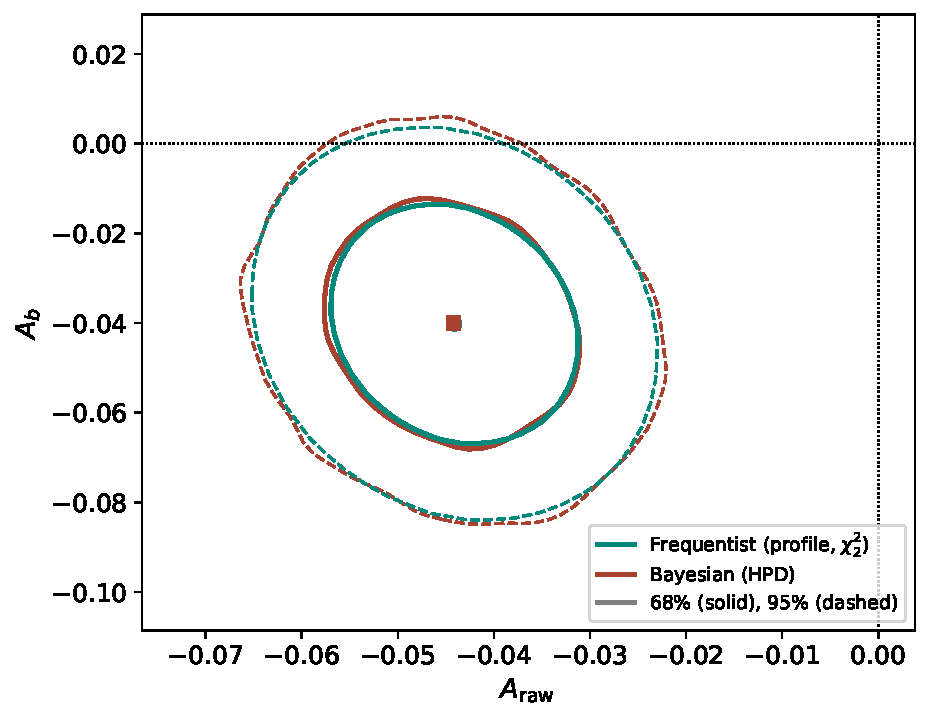
\includegraphics[width=\columnwidth]{figures/validation_region_Ab.pdf}
\caption{$68\%$ (solid) and $95\%$ (dashed) regions in $(A,A_b)$: Frequentist, from the profile likelihood with $\chi^2_2$ thresholds, and Bayesian, highest-posterior-density regions of the chain. Dots: best-fit and posterior median.}
\label{fig:checks_region}
\end{figure}

\subsection{Bayesian and Frequentist Intervals at Low Statistics}
\label{sec:bayes_lowstat}
\emph{In short: credible and confidence intervals coincide for $\sim2\times10^4$ candidates with flat priors, and stay equal, in value and coverage, down to $50$ candidates.}
With $\sim$$2\times10^4$ candidates the posterior is Gaussian and, with flat priors, the Bayesian and Frequentist results coincide by construction (Sec.~\ref{sec:bayes_posterior}). To find where they could differ, the same likelihood was analysed with both methods on toy-MC datasets of $N=50$, $150$, $500$ and $2000$ candidates, $300$ for each size. The model is the six-parameter one of Sec.~\ref{sec:bayes_minimal} (Gaussian signal, one exponential background shared by the charges), which stays identifiable down to a few tens of events; the parameters are those of its fit to the data, with the yields rescaled. Each replica is analysed with the MCMC (median and equal-tailed credible intervals) and by maximum likelihood with \texttt{iminuit} (Hesse intervals, and Minos intervals from the profile likelihood and Wilks' theorem).

The two methods agree at every size (Fig.~\ref{fig:bayes_lowstat}). The coverages of the three intervals are compatible with nominal and with each other, the posterior median and the maximum-likelihood estimate differ on average by $5\%$ of the statistical uncertainty at $N=50$ and by less above, and the credible intervals stay symmetric (at $N=50$ the shortest chain is only $\approx10$ autocorrelation times long, so the Monte Carlo error on the interval endpoints is larger there). The asymmetry is a ratio of Poisson yields, whose likelihood is close to Gaussian already with a few tens of signal events: in this problem flat-prior credible intervals and profile-likelihood confidence intervals give the same answer, and Wilks' theorem holds, down to $N=50$. The two approaches differ in what the interval means and in hypothesis testing (Sec.~\ref{sec:bayes_factor}), not in the numbers. At $N=2000$ all three intervals over-cover slightly ($0.98$--$0.99$ for the 95\% interval); since the effect is the same for the three methods, it is a feature of this set of replicas rather than of either inference.

\begin{figure*}[t]
\centering
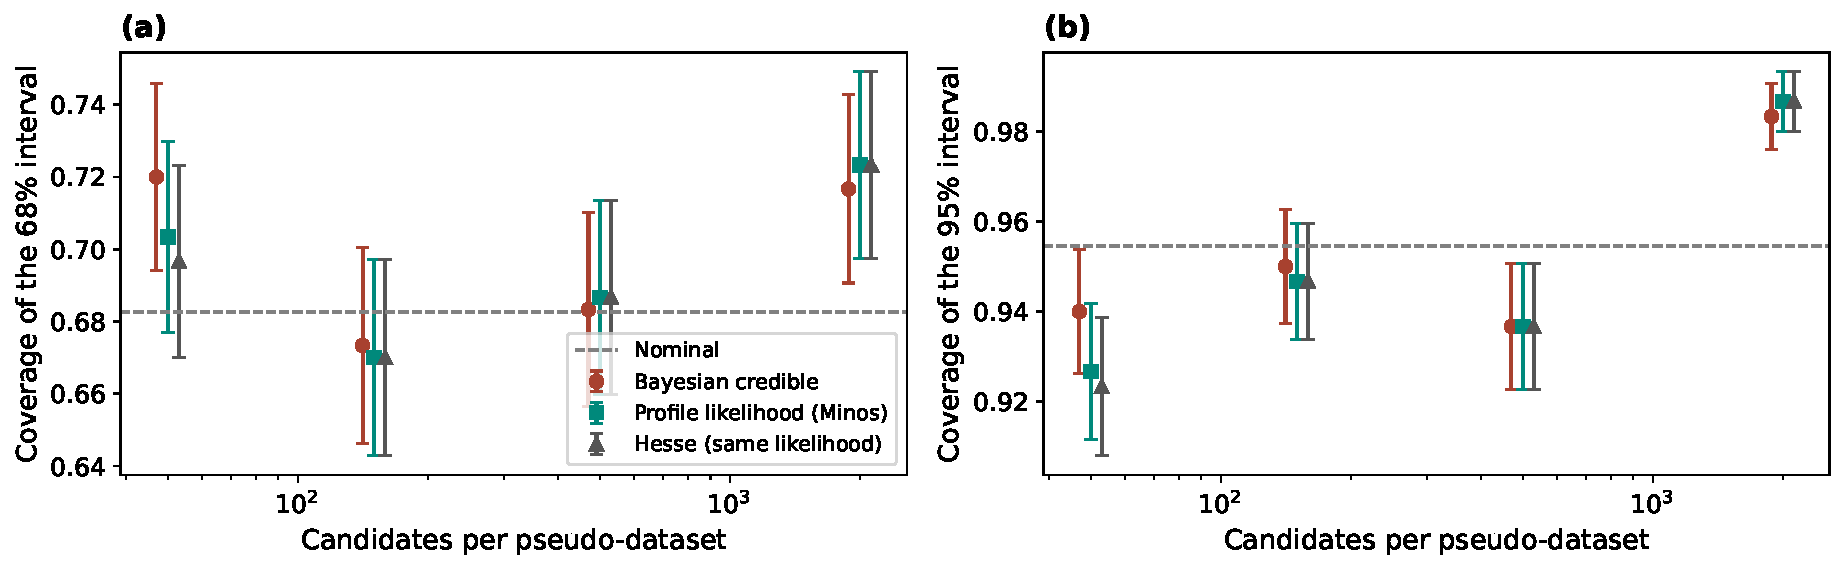
\includegraphics[width=0.95\textwidth]{figures/bayes_nominal_lowstat.pdf}
\caption{Coverage of the (a) 68\% and (b) 95\% intervals on $A$ vs the number of candidates, for the Bayesian credible interval, the profile-likelihood (Minos) interval and the Hesse interval of the same likelihood; 300 toy-MC datasets per point, binomial uncertainties. The dashed lines mark the nominal coverage ($1\sigma$, $2\sigma$; the Bayesian 95\% interval is the 2.5--97.5\% one).}
\label{fig:bayes_lowstat}
\end{figure*}

\FloatBarrier

\section{Discussion and Conclusions}
\label{sec:conclusions}
\label{app:conclusions}
\emph{In short: two inference frameworks give the same raw asymmetry, $\Araw=-0.044\pm0.009\,(\text{stat})\pm0.007\,(\text{syst})$, $5.2$ standard deviations from zero, with validated intervals; what separates them is the meaning of the numbers and the tests, not their values.}
On this problem the Frequentist profile-likelihood fit and the Bayesian posterior are equivalent in value, uncertainty and coverage: with a common selection and mass model they give $\Araw=-0.0441\pm0.0085\pm0.0072$ and $-0.0443\pm0.0085\pm0.0070$ (statistical, systematic), a nonzero asymmetry at $5.2$ standard deviations, stable under the thirteen variants (the dominant systematic contribution is the particle-identification requirement) and concentrated in the Dalitz region of the published analysis outside the $\phi(1020)$ ($-0.234\pm0.025$ against $-0.239\pm0.020$).
The numbers coincide, the statements do not. The credible interval states that $A$ lies in $[-0.0528,-0.0358]$ with $68\%$ probability given the data and the prior; the confidence interval $[-0.0526,-0.0356]$ is the set of values that the data do not reject, and its $68\%$ is a property of the procedure that the bootstrap and the toy experiments verified\appref{app:ext_comp}. The Frequentist test of $A=0$, $p=2\times10^{-7}$, is independent of the prior; the Bayes factor, $BF_{10}\approx9\times10^3$, depends on its width (Sec.~\ref{sec:bayes_factor}), and for $A_b=-0.040\pm0.018$ a Frequentist test would call $2.3\sigma$ a hint while $BF_{01}\approx3.5$ mildly favors $A_b=0$. The Frequentist fit adds an unbiased estimator at the minimum variance bound; the Bayesian analysis adds sampling diagnostics and a posterior predictive check.
The published analysis~\cite{lhcb_cpv_2013} finds $-0.060\pm0.007$ on a larger sample with a richer model\appref{app:ext_comp}; with the same $D^0$ veto the Bayesian fit gives $-0.0496\pm0.0088$, within $0.93\sigma$. The raw asymmetry is not the $CP$ asymmetry, $\ACP\approx\Araw-A_P-A_D$ (Eq.~\eqref{eq:acp}): the $5.2\sigma$ here is the significance of a nonzero raw asymmetry, not of $CP$ violation. Three limitations bound the result\appref{sec:limitations}: no tested model reaches $\chi^2/\mathrm{ndof}\approx1$, although $\Araw$ does not depend on the signal shape; no production or detection correction is applied; and the local Dalitz-plane asymmetries are counts without background subtraction. A machine-learning selection leaves $\Araw$ unchanged within its statistical spread (Sec.~\ref{sec:ml}), and the natural next step is a control-channel correction.
\subsection{Lessons of Each Method}
\emph{In short: the Frequentist fit gives intervals with nominal coverage and an unbiased estimator; the Bayesian one the same interval with flat priors plus diagnostics to check, a Bayes factor that depends on the prior and a predictive check; the ML selection leaves $\Araw$ unchanged.}
Each method taught something specific.
\begin{itemize}[leftmargin=*,itemsep=2pt]
\item \emph{Frequentist.} With the other eleven parameters profiled, Wilks' theorem gives a $68\%$ interval with the nominal coverage ($68.4\pm1.5\%$ in $1000$ bootstrap replicas of the data, $0.70\pm0.01$ and $0.95\pm0.01$ in toy-MC experiments from the fitted model, where the estimator is also unbiased and reaches the minimum variance bound), and the Hesse and Minos uncertainties agree, so the likelihood is parabolic in $A$ at this sample size.
\item \emph{Bayesian.} With $\sim2\times10^4$ candidates and flat priors the posterior is the likelihood, and the credible interval coincides with the confidence interval and has the same coverage in toy experiments. The Bayesian analysis adds what the Frequentist one lacks: sampling diagnostics that must be checked rather than assumed (autocorrelation time, dispersed starts, label switching of the two background slopes), a Bayes factor that depends on the prior width, and a posterior predictive check whose charge statistics, being fitted, have no power.
\item \emph{Machine learning (Sec.~\ref{sec:ml}).} Weak labels from the mass spectrum are enough to train classifiers of test AUC $\simeq0.86$, but the selection does not improve the precision on $\Araw$ in a sample with little background, and it cannot remove the misidentified decays that peak under the signal. Its value is as an independent test of the stability of $\Araw$ under a different selection and, with $K$-means, as an adaptive description of the Dalitz plane that agrees with the fixed binning.
\end{itemize}
\subsection{Limitations and Future Work}
\label{sec:limitations}
\emph{In short: no signal model reaches $\chi^2/\mathrm{ndof}\approx1$ although $\Araw$ does not depend on it, the machine-learning labels are weak and imbalanced, $\Araw$ is not corrected for production and detection asymmetries, and the natural next step is a control-channel correction.}
Several modeling choices and known weaknesses limit how far the results of Secs.~\ref{sec:bayesian}--\ref{sec:syst} and Sec.~\ref{sec:ml} can be pushed, and are collected here rather than scattered through the results sections.
On the mass fits (Secs.~\ref{sec:bayesian}--\ref{sec:syst}):
\begin{itemize}[leftmargin=*,itemsep=2pt]
\item no tested signal model reaches $\chi^2/\mathrm{ndof}\approx1$ (the best, a Crystal Ball, gives $131.0/86$, Sec.~\ref{sec:bayes_gof}; the $p$-value of the binned $\chi^2$ is $5\times10^{-6}$ at $10\,\MeV$ and $0.03$ at $2.5\,\MeV$, Sec.~\ref{sec:validation_gof}), although $\Araw$ does not depend on the signal shape;
\item the systematic uncertainty, $0.007$, is almost as large as the statistical one and is dominated by a PID variant that a finer scan identifies as a statistical fluctuation (Sec.~\ref{sec:syst}); it is therefore conservative, but the combination rule cannot separate the two;
\item the Savage-Dickey Bayes factor of Sec.~\ref{sec:bayes_factor} relies on a Gaussian approximation of the posterior far in its tail and depends on the prior width, although the conclusion (decisive evidence against $A=0$) is robust;
\item the toy-MC coverage check of Sec.~\ref{sec:bayes_toymc} is a closure test and cannot detect model misspecification;
\item the local Dalitz asymmetries (Secs.~\ref{sec:bayes_dalitz} and \ref{sec:ml_kmeans}) use a coarse partition, a mass-window cut rather than a proper background subtraction, and no correction for momentum-dependent detection asymmetries.
\end{itemize}
On the machine-learning side (Sec.~\ref{sec:ml}): the weak labels are imbalanced ($1940$ background-like vs.\ $15{,}130$ signal-like candidates, Sec.~\ref{sec:ml_labels}), and the test set contains only $388$ background-like candidates, so differences in test AUC below $\sim$0.01 cannot be resolved; the three uncertainty estimators differ by a factor $\sim$3.5 in scale and measure different sources of variability (Sec.~\ref{sec:ml_uncertainty}); and the score-based selection changes the composition of the background, keeping the partially reconstructed and other non-combinatorial $B$ decays that the nominal model does not describe (Sec.~\ref{sec:ml_stability}); removing the momentum features does not help, since the weak labels cannot separate these decays from the signal.
More generally, no detector-level systematic correction (selection efficiency, production asymmetry) is applied anywhere in this work, so $\Araw$ as reported throughout is explicitly \emph{not} a measurement of $\ACP$; in the language of unfolding, the measured asymmetry is the folded one, and mapping it back to the true asymmetry would require the response of the detector (acceptance, charge-dependent efficiency, interaction of kaons with matter), which is not available in this record (Sec.~\ref{sec:comparison}). The published analysis corrects for $A_P+A_D$ with $B^\pm\to J/\psi K^\pm$, $J/\psi\to\mu^+\mu^-$~\cite{lhcb_cpv_prd2023}, which is not part of this record; the $J/\psi\to K^+K^-$ decays inside our sample cannot replace it, since this mode is rare and the $568$ candidates under the $B$ peak in the $J/\psi$ band are dominated by charmless decays ($A_{\mathrm{count}}=-0.165\pm0.041$, a local Dalitz-plot asymmetry rather than a control measurement).
The most natural next steps, in rough priority order, are: correcting $\Araw$ for the production and detection asymmetries with a control channel such as $B^\pm\to J/\psi K^\pm$, $J/\psi\to\mu^+\mu^-$; replacing the fixed-cut local Dalitz asymmetries (both binned, Sec.~\ref{sec:bayes_dalitz}, and $K$-means, Sec.~\ref{sec:ml_kmeans}) with a proper sWeight-based background subtraction; and an explicit model of the partially reconstructed and other non-combinatorial $B$ backgrounds, which would also make an ML-selected sample usable for a fit.
\FloatBarrier

\section{Code and Data Availability}
\label{sec:code}
\emph{In short: Python code with the package versions listed here; Frequentist, Bayesian and machine-learning code and notebooks are in the accompanying repository.}
All code is written in Python $\geq$3.12, with \texttt{scikit-learn}~\cite{sklearn} for the classical machine-learning models and \texttt{TensorFlow}/\texttt{Keras}~\cite{tensorflow} for the neural networks. Key package versions: \texttt{uproot 5.7}, \texttt{iminuit 2.32.0}, \texttt{emcee 3.1.6}, \texttt{corner 2.3.0}, \texttt{scikit-learn 1.9}, \texttt{tensorflow 2.21.0}, \texttt{keras 3.15.1}, \texttt{scipy 1.18}, \texttt{numpy 2.4}, \texttt{pandas 3.0}.
The dataset is the CERN Open Data record \href{https://opendata.cern.ch/record/4900}{4900} ("Matter Antimatter Differences -- B meson decays to three hadrons"). The analysis code is available in the accompanying repository, in \texttt{Code\_general/Frequentist/} (notebook \texttt{06\_frequentist\_fit\_stability\_systematics}: the data, the simultaneous and separate fits, the profile likelihood and the bootstrap coverage, the stability scans, the systematic study common to the Bayesian analysis, the charm vetoes and the Dalitz plane; \texttt{lhcb\_freq.py} with the functions; \texttt{freq\_validation.py} with the toy-MC experiments, profile likelihoods, confidence belt and bootstrap studies of Sec.~\ref{sec:validation}; \texttt{make\_figures.py} for the figures), \texttt{Code\_general/Bayesian/} (notebooks \texttt{01\_bayes\_mass\_fit\_and\_asymmetry}: nominal fit, Bayes factors, systematic study, toy-MC closure test, magnet polarities and Dalitz plane; \texttt{02\_bayes\_model\_checks\_and\_priors}: posterior predictive checks, convergence diagnostics, sensitivity to the priors and comparison with the profile likelihood; \texttt{03\_bayes\_vs\_frequentist\_low\_statistics}: the two approaches at low statistics; the mass model, the sampler and the toy generator are in \texttt{bayes\_model.py}), and \texttt{Code\_general/Machine\_Learning/} (notebooks \texttt{04\_ml\_signal\_background\_classifiers}: weak labels, classifiers, calibration, uncertainty and hyperparameters; \texttt{05\_ml\_selection\_and\_local\_asymmetry}: effect of the selection on $\Araw$, K-means and null tests on the Dalitz plane, comparison with the published analysis; helper functions in \texttt{ml\_tools.py}). Each of these notebooks opens with a table of the sections and figures of this paper that it produces and generates those figures from its saved results, so that they can be rebuilt without repeating the long computations; the common style is in \texttt{Code\_general/plot\_style.py}. The figures of the Frequentist analysis are produced from its saved results by \texttt{regen\_figures\_validation.py}, \texttt{regen\_figures\_systematics.py} and \texttt{regen\_figures\_extras.py} in the figures directory of the report. All random numbers are generated with fixed seeds, so the toy-MC experiments can be reproduced.

\section{Author Contributions}
\label{sec:contributions}
Marco Belotti led the Frequentist analysis (Sec.~\ref{sec:frequentist}): mass model, likelihood fits, and profile-likelihood confidence interval. Giacomo Moretti led the Bayesian analysis (Sec.~\ref{sec:bayesian}): model definition, MCMC sampling, convergence diagnostics, Bayes factor, and the associated systematic/goodness-of-fit studies. The common nominal model, the systematic study (Sec.~\ref{sec:syst}), the machine learning analysis and the comparison of the three methods on the ML-selected sample (Sec.~\ref{sec:ml}), the toy-MC validation, the Dalitz-plot analyses, and the final cross-method comparison (Sec.~\ref{sec:comparison}) were carried out jointly. Both authors contributed to the manuscript.

\appendix
\section{Notation}
\label{sec:notation}
The symbols used in the text are listed in Table~\ref{tab:notation}.

\begin{table}[h]
\centering
\begin{tabular}{ll}
\toprule
Symbol & \pcell{6.2cm}{Meaning} \\
\midrule
$\Araw$ & \pcell{6.2cm}{raw charge asymmetry $(N^--N^+)/(N^-+N^+)$ of the signal, parameter $A$ of the fit} \\
$\ACP$, $A_P$, $A_D$ & \pcell{6.2cm}{CP asymmetry; production asymmetry of $B^\pm$; detection asymmetry} \\
$A_{\mathrm{count}}$ & \pcell{6.2cm}{counting asymmetry of all candidates of a sample} \\
$A_b$ & \pcell{6.2cm}{asymmetry of the background yields} \\
$N_s$, $N_b$ & \pcell{6.2cm}{signal and background yields (both charges)} \\
$\mu$, $\sigma$ & \pcell{6.2cm}{mean and width of the Gaussian signal} \\
$\lambda_{1,2}^\pm$, $f_\pm$ & \pcell{6.2cm}{slopes and fraction of the double-exponential background, per charge} \\
$\theta$ & \pcell{6.2cm}{vector of the twelve parameters} \\
$\mathcal L$, $\pi$ & \pcell{6.2cm}{likelihood and prior} \\
$q(A)=2\Delta\mathrm{NLL}$ & \pcell{6.2cm}{profile likelihood ratio of $A$; $t(A_{\mathrm{true}})$ at the injected value} \\
$Z$, $p$ & \pcell{6.2cm}{significance and $p$-value of the test of $A=0$} \\
$BF_{01}$, $BF_{10}$ & \pcell{6.2cm}{Bayes factor of $A=0$ against $A$ free, and its inverse} \\
$p_B$ & \pcell{6.2cm}{posterior predictive $p$-value} \\
$\sigma_B$ & \pcell{6.2cm}{expected spread of the shift between nested samples, $\sqrt{|\sigma_{\mathrm{var}}^2-\sigma_{\mathrm{nom}}^2|}$} \\
$N/\tau$ & \pcell{6.2cm}{chain length in integrated autocorrelation times} \\
$S_i$, $S_k$ & \pcell{6.2cm}{local significance of a Dalitz bin or cluster with respect to the global asymmetry} \\
\bottomrule
\end{tabular}
\caption{Main symbols used in the text.}
\label{tab:notation}
\end{table}



\bibliography{biblio}

\end{document}
